% main.tex
% Fichero principal de transparencias (incluye a todos los dem�s).

% Compilar a .pdf con LaTeX (pdflatex)
% Es necesario instalar Beamer (paquete latex-beamer en Debian)
%

% Gr�ficos:
% Los gr�ficos pueden suministrarse en PNG, JPG, TIF, PDF, MPS
% Los EPS deben convertirse a PDF (usar epstopdf)
%
\documentclass{beamer}
\usetheme{Warsaw}
\beamertemplatenavigationsymbolsempty
\setbeamertemplate{headline}{}
\useoutertheme{infolines}
%\usebackgroundtemplate{
\includegraphics[width=\paperwidth]{format/libresoft-bg-soft.png}}
\usepackage[spanish]{babel}
\usepackage[latin1]{inputenc}
\usepackage{graphics}
\usepackage{amssymb} % Simbolos matematicos

\newcommand{\asignatura}{Servicios y Aplicaciones Telem�ticas}
\newcommand{\grado}{Grado en Ingenier�a Tecnolog�as de Telecomunicaci�n (URJC)}
\newcommand{\curso}{2014-15}
\newcommand{\horario}{M (11:00-13:00) y J (11:00-13:00)}

%\definecolor{libresoftgreen}{RGB}{162,190,43}
%\definecolor{libresoftblue}{RGB}{0,98,143}

%\setbeamercolor{titlelike}{bg=libresoftgreen}

%% Metadatos del PDF.
\hypersetup{
  pdftitle={\asignatura~\curso},
  pdfauthor={Jes�s M. Gonz�lez Barahona, Gregorio Robles},
  pdfcreator={GSyC, Universidad Rey Juan Carlos},
  pdfproducer=PDFLaTeX,
  pdfsubject={\asignatura~\curso},
}
%%


%%%%%%%%%%%%%%%%%%%%%%%%%%%%%%%%%%%%%%%%%%%%%%%%%%%%%%%%%%%%%%%%
%%%%%%%%%%%%%%%%%%%%%%%%%%%%%%%%%%%%%%%%%%%%%%%%%%%%%%%%%%%%%%%%
% include-only                                                 %
%%%%%%%%%%%%%%%%%%%%%%%%%%%%%%%%%%%%%%%%%%%%%%%%%%%%%%%%%%%%%%%%
%%%%%%%%%%%%%%%%%%%%%%%%%%%%%%%%%%%%%%%%%%%%%%%%%%%%%%%%%%%%%%%%
\includeonly{presentacion-sat-saro,cookies,python}
%\includeonly{cookies}
%\includeonly{rest}
%\includeonly{mvc}
%\includeonly{xml}
%\includeonly{css}
%\includeonly{www-novedades}
%\includeonly{www-applications}
%\includeonly{caso-comunidades}
%\includeonly{complex-www-sites}
%\includeonly{ldap,webdav}
%\includeonly{webdav}
%\includeonly{xml,webdav}
%\includeonly{streaming}
%\includeonly{streaming, sdp}
%\includeonly{streaming,smil}
%\includeonly{smil}
%\includeonly{security-intro,security-ipsec,security-ssl}
%\includeonly{webdav,security-ssl}

%% Pr�cticas
%\includeonly{python}
%\includeonly{sql}
%\includeonly{django}


\AtBeginSection[]
{
\begin{frame}<beamer>
\begin{center}
{\Huge \insertsection}
\end{center}
\end{frame}
}


\begin{document}

\title[\asignatura~\curso]{\asignatura~(\curso)}
\subtitle{\grado}
\author[GSyC]{Jes�s M. Gonz�lez Barahona, Gregorio Robles Mart�nez}
\institute[http://cursosweb.github.io/]{\url{http://cursosweb.github.io} \\
GSyC, Universidad Rey Juan Carlos}

%\date{Enero 2015}


\frame{
\maketitle

\begin{center}

\includegraphics[width=6cm]{format/gsyc-urjc}
\end{center}
}


% Si el titulo o el autor se quieren acortar para los pies de p�gina
% se pueden redefinir aqu�:
%\title{Titulo corto}
%\author{Autores abreviado}


%% LICENCIA DE REDISTRIBUCION DE LAS TRANSPAS
\frame{
~
\vspace{3cm}

\begin{flushright}
\copyright 2002-2015 Jes�s M. Gonz�lez Barahona, Gregorio Robles y
Jorge Ferrer. \\

Algunos derechos reservados. Este art�culo se distribuye bajo
la licencia ``Reconocimiento-CompartirIgual 3.0 Espa�a'' de Creative Commons,
disponible en \\
{\small \url{http://creativecommons.org/licenses/by-sa/3.0/es/deed.es}}

Este documento (o uno muy similar) est� disponible en \\
\url{http://cursosweb.github.io}
\end{flushright}
}
%%

%\frame{
%\tableofcontents
%}

%%%%%%%%%%%%%%%%%%%%%%%%%%%%%%%%%%%%%%%%%%%%%%%%%%%%%%%%%%%%%%%%
%%%%%%%%%%%%%%%%%%%%%%%%%%%%%%%%%%%%%%%%%%%%%%%%%%%%%%%%%%%%%%%%
% lista de temas                                               %
%%%%%%%%%%%%%%%%%%%%%%%%%%%%%%%%%%%%%%%%%%%%%%%%%%%%%%%%%%%%%%%%
%%%%%%%%%%%%%%%%%%%%%%%%%%%%%%%%%%%%%%%%%%%%%%%%%%%%%%%%%%%%%%%%


\section{Presentaci�n de la asignatura}

%%---------------------------------------------------------------

\begin{frame}
\frametitle{Datos, datos, datos}

\begin{itemize}
\item Profesores:
  \begin{itemize}
  \item Jes�s M. Gonz�lez Barahona (jgb @ gsyc.urjc.es)
  \item Gregorio Robles (grex @ gsyc.urjc.es)
  \end{itemize}
\item Grupo de Sistemas y Comunicaciones (GSyC)
\item Despachos: 101 y 110 Departamental III
\item Horario: \horario
\item Tutor�a: Horario por definir (en los Laboratorios)
\item Laboratorio 209 Laboratorios III
\end{itemize}

\begin{flushright}
  Campus virtual: {\small \url{http://aulavirtual.urjc.es}} \\
  Cursos web: {\small \url{http://cursosweb.github.io}} \\
  GitLab de la ETSIT: {\small \url{http://gitlab.etsit.urjc.es}} \\
\end{flushright}

\end{frame}


%-----------------------    ---------------------------------
\usebackgroundtemplate{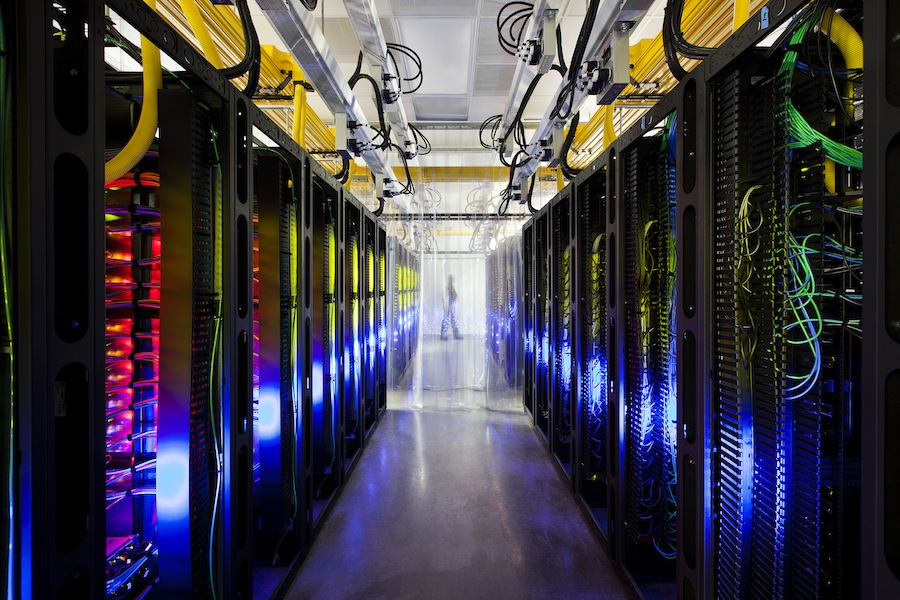
\includegraphics[width=12.8cm]{figs/internet.jpg}}
% http://cdn6.yorokobu.es/wp-content/uploads/Council-Bluffs-Network-Room.jpg

\begin{frame}
\frametitle{�De qu� va todo esto?}

\vspace{3.5cm}

\begin{center}
\color{white}
\Huge {\bf Entendiendo c�mo funciona la web}
\end{center}

\end{frame}
\usebackgroundtemplate{}


%%---------------------------------------------------------------

\begin{frame}
\frametitle{En concreto...}

{\Large
\begin{itemize}
\item C�mo se construyen los sistemas reales \\
  que se usan en Internet
  \item Qu� tecnolog�as se est�n usando
  \item Qu� esquemas de seguridad hay
  \item C�mo encajan las piezas
  \item En la medida de lo posible, ``manos en la masa''
\end{itemize}
}

\end{frame}


%%---------------------------------------------------------------

\begin{frame}
\frametitle{Ejemplos}

{\Large
\begin{itemize}
  \item �Qu� es una aplicaci�n web?
  \item �Qu� es una sesi�n?
  \item �C�mo construir un servicio REST?
  \item Acaba con la magia de los servicios web
  \item �C�mo se hace un servicio basado en contenidos?
\end{itemize}
}
\end{frame}

%-----------------------    ---------------------------------
\usebackgroundtemplate{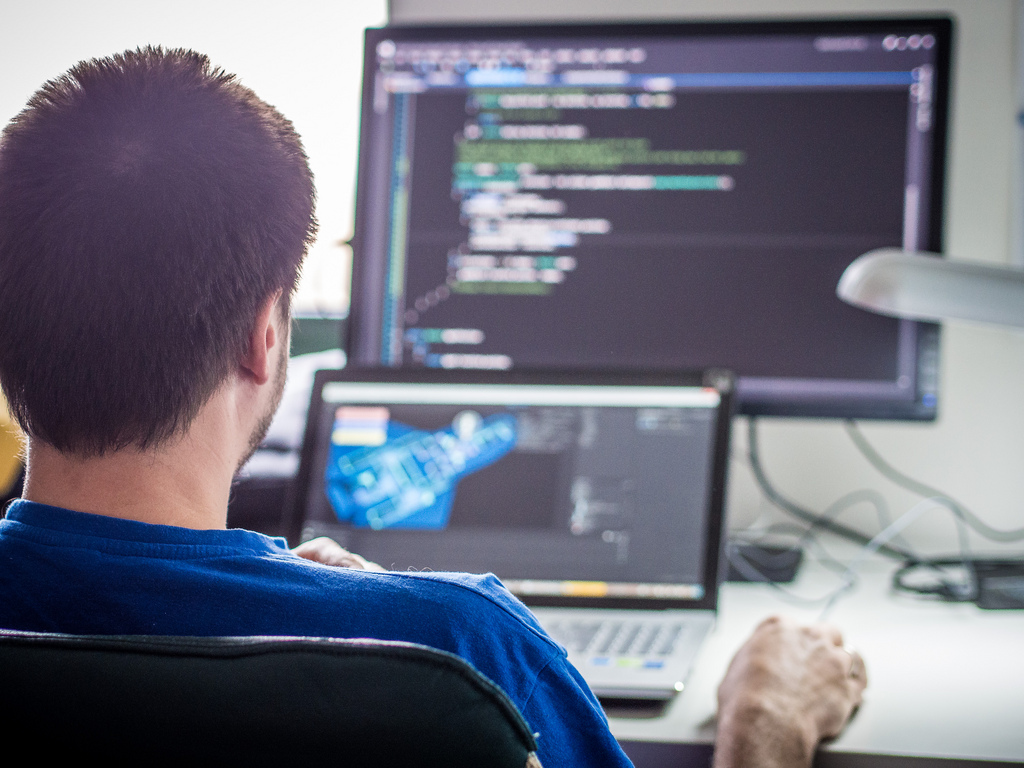
\includegraphics[width=13cm]{figs/programmer.jpg}}
% http://www.openweigh.com/assets/programmer-e898f9c9a43ecd208f1f1df347713e6e.jpg

\begin{frame}
\frametitle{Fundamentos de la asignatura}

\vspace{3.8cm}

\begin{center}
\color{red}
\Huge {\bf La programaci�n es el lenguaje de la tecnolog�a}
\end{center}

\end{frame}
\usebackgroundtemplate{}

%-----------------------    ---------------------------------

\begin{frame}
\frametitle{Lenguaje de Programaci�n: Python}

\begin{center}
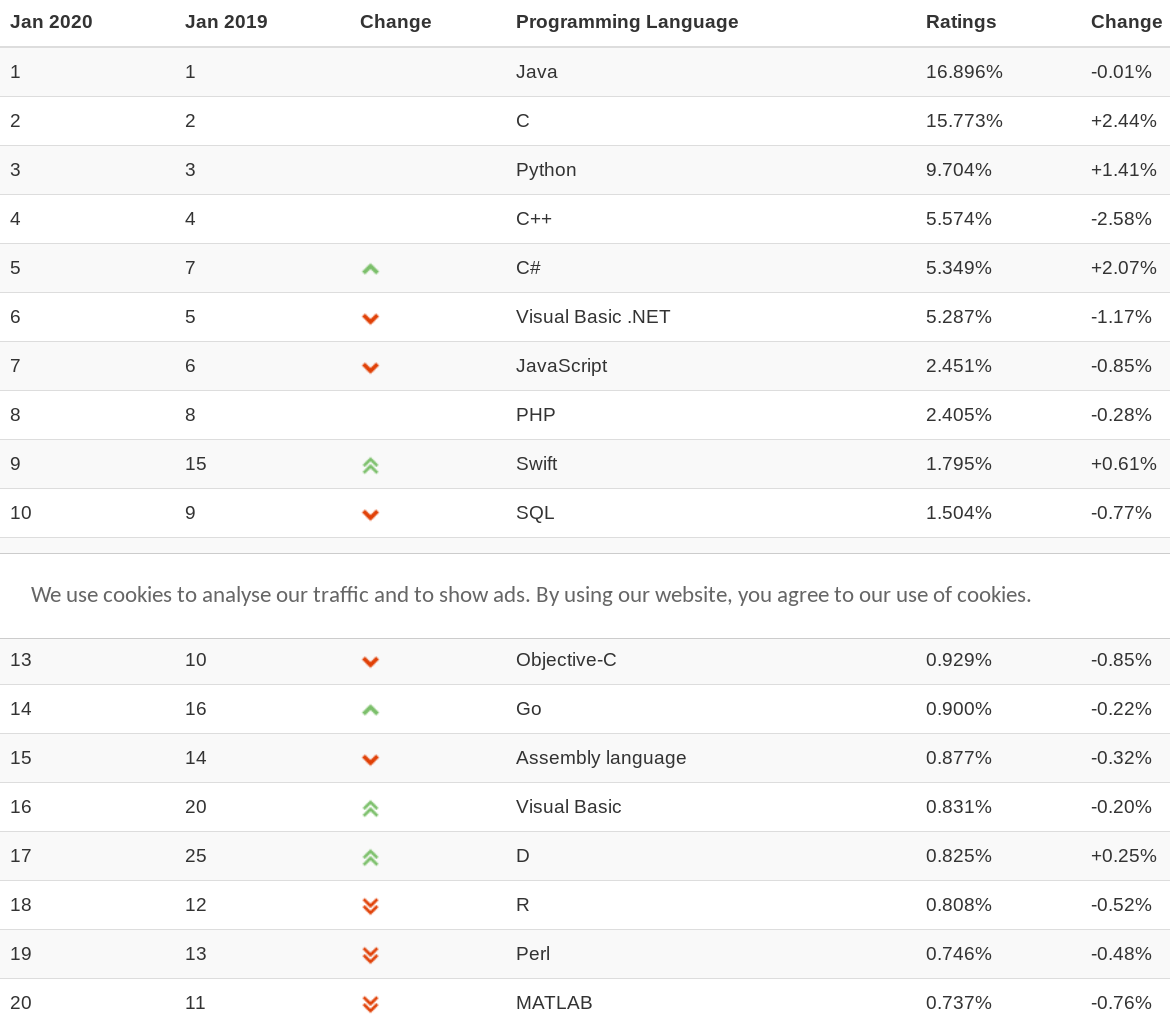
\includegraphics[width=5cm]{figs/2020-most-popular-lang-tiobe}
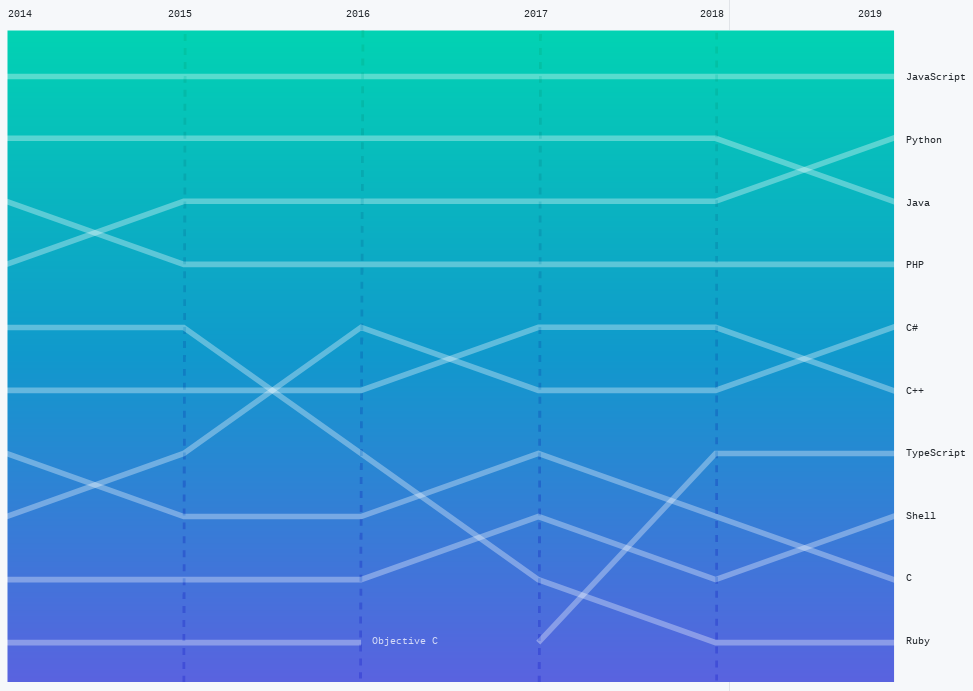
\includegraphics[width=6cm]{figs/2019-most-popular-lang-github}
\end{center}

\begin{center}
  {\Large Primer Mandamiento: \\ Amar�s Python por encima de (casi) todo.} \\
  TIOBE (enero 2020) ~~~~ GitHub (noviembre 2019) \\
\end{center}


\end{frame}
\usebackgroundtemplate{}


%-----------------------    ---------------------------------

\begin{frame}
\frametitle{Plataforma: Django}

\begin{center}
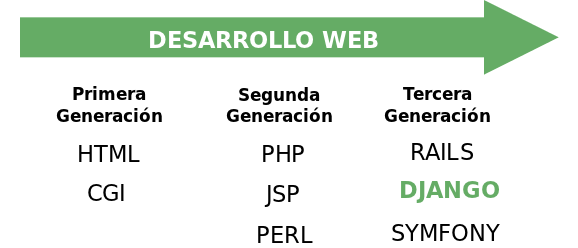
\includegraphics[width=11cm]{figs/django.png}
% http://www.maestrosdelweb.com/images/2012/04/desarrolloweb.png
\end{center}

\begin{center}
\Large Segundo Mandamiento: \\ No tomar�s el nombre de Django en vano.
\end{center}


\end{frame}
\usebackgroundtemplate{}

%%---------------------------------------------------------------

\begin{frame}
\frametitle{Metodolog�a}

{\Large
\begin{itemize}
\item Objetivo principal: conceptos b�sicos de construcci�n de sitios web modernos
\item Clases de teor�a y de pr�cticas, pero...
\item Teor�a en pr�cticas, pr�cticas en teor�a
\item Uso de resoluci�n de problemas para aprender
\item Fundamentalmente, entender lo fundamental
\end{itemize}
}
\end{frame}

%-----------------------    ---------------------------------
\usebackgroundtemplate{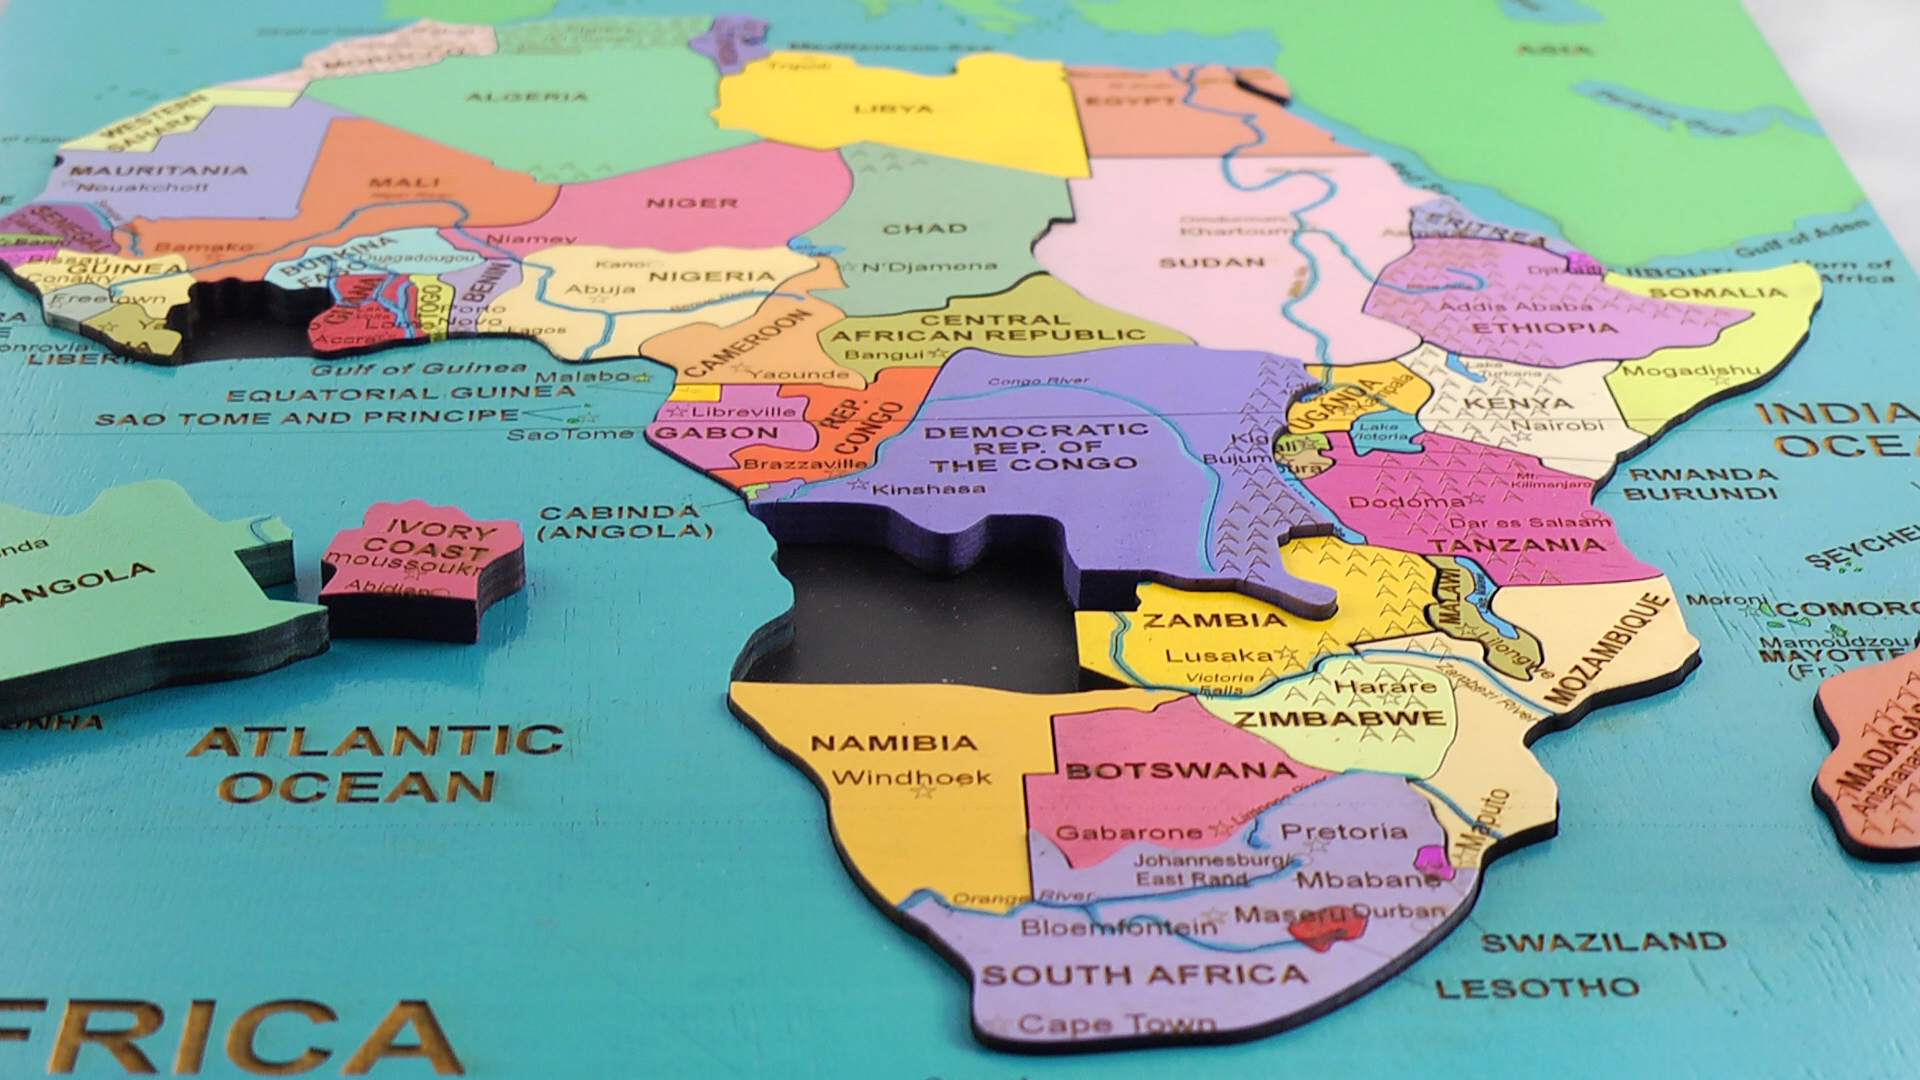
\includegraphics[width=13cm]{figs/africa.jpg}}
% http://www.funlearningcompany.com/wp-content/themes/smallbiz/images/Map100.jpg

\begin{frame}
\frametitle{Fundamentos de la asignatura}

\vspace{5.4cm}

\begin{center}
\Huge Aprender no puede ser aburrido
\end{center}

\end{frame}
\usebackgroundtemplate{}

%%---------------------------------------------------------------

\begin{frame}
\frametitle{Las Clases}

\begin{itemize}
  \item Empezamos en punto
  \item 10 minutos con un tema motivacional
  \begin{itemize}
    \item Gadgets tecnol�gicos
    \item Aplicaciones
    \item Cuestiones interesantes
    \item \dots
  \end{itemize}
  \item Generalmente, explicaci�n de los conceptos m�s importantes y luego
realizaci�n de ejercicios
  \item No hay descanso
  \item Ejercicios para hacer fuera de clase (y entregar)
\end{itemize}

\end{frame}



%-----------------------    ---------------------------------
\usebackgroundtemplate{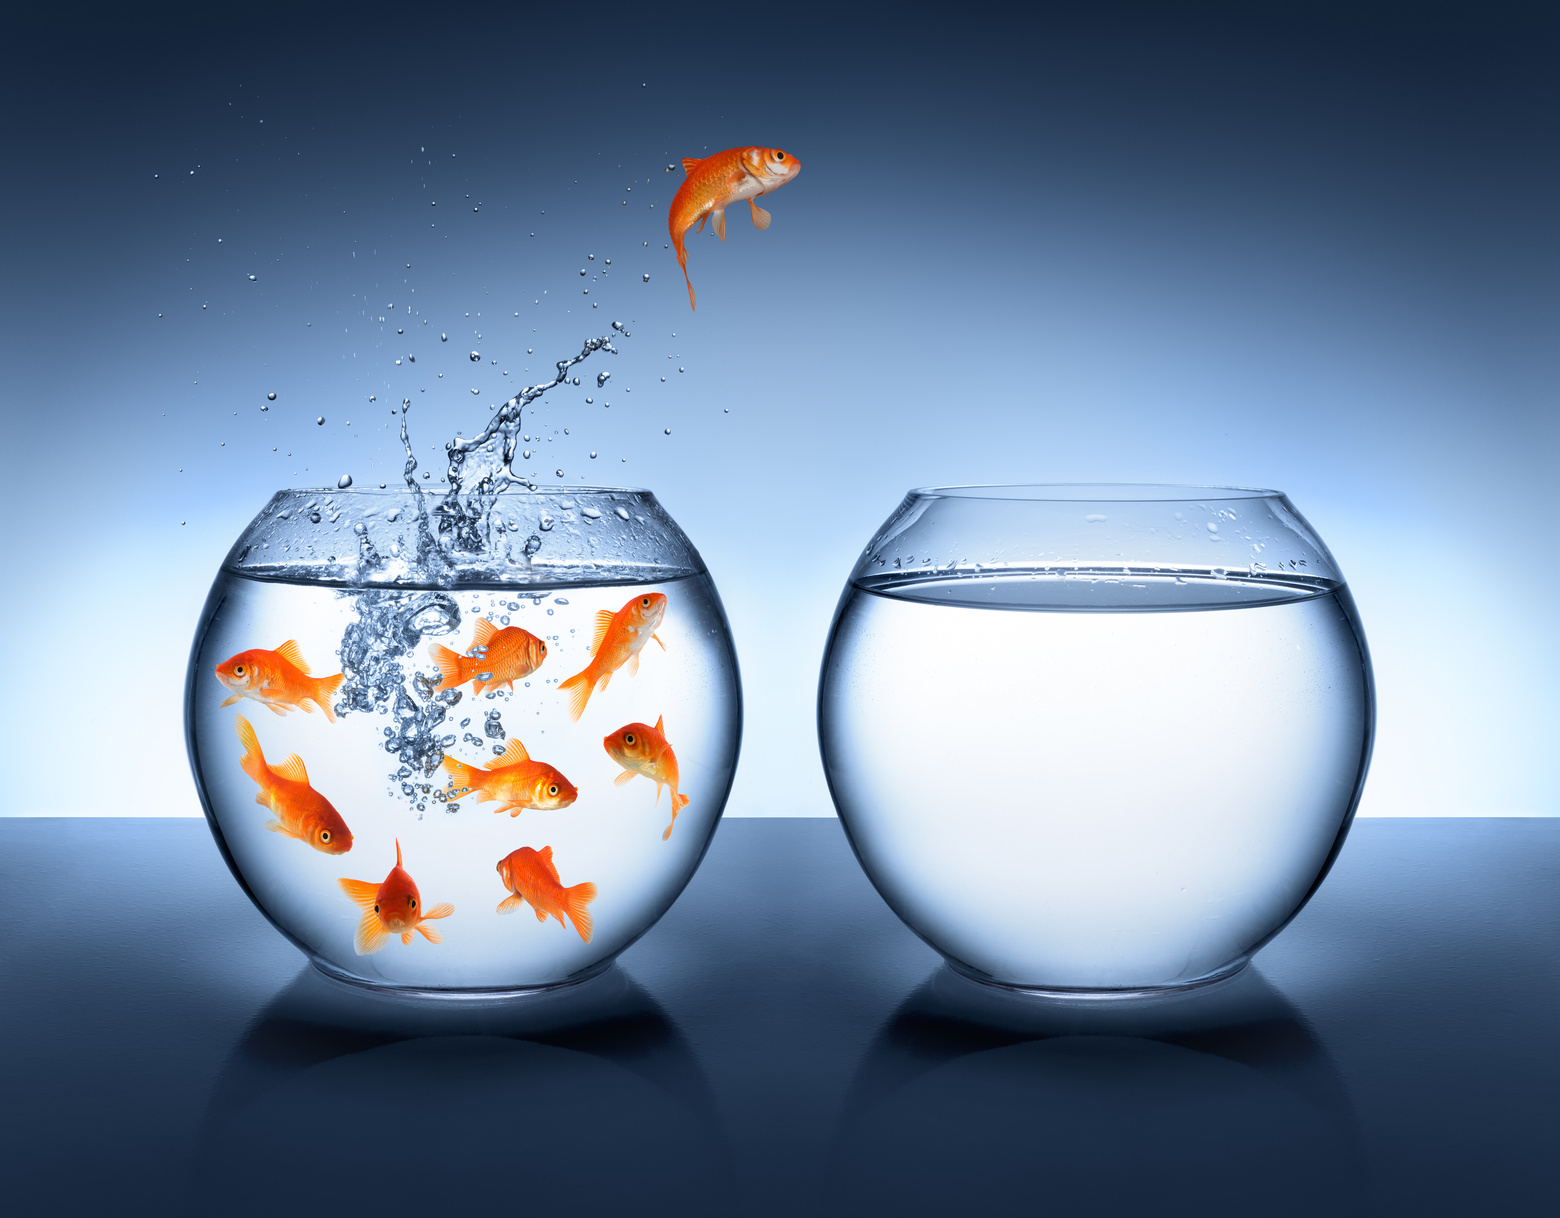
\includegraphics[width=13.5cm]{figs/challenge.jpg}}
% http://ichallenge.com/wp-content/uploads/2014/08/challenge-6.jpg

\begin{frame}
\frametitle{Fundamentos de la asignatura}

\vspace{-2.75cm}

\begin{center}
\Huge El estudiante es el centro del aprendizaje
\end{center}

\end{frame}
\usebackgroundtemplate{}



%%---------------------------------------------------------------

\begin{frame}
\frametitle{Evaluaci�n}

\begin{itemize}
\item Micropr�cticas diarias (entrega foro/GitLab): 0 a 1
\item Minipr�cticas preparatorias: 0 a 1
\item Pr�ctica final (obligatorio): 0 a 2.
\item Opciones y mejoras pr�ctica final: 0 a 3
\item Teor�a (obligatorio): 0 a 5.
\item Nota final: Suma de notas, moderada por la interpretaci�n del profesor
\item M�nimo para aprobar:
      \begin{itemize}
      \item Aprobado en teor�a (2.5) y pr�ctica final (1), y
      \item 5 puntos de nota final en total
      \end{itemize}
\end{itemize}

\end{frame}

%%---------------------------------------------------------------

\begin{frame}
\frametitle{Evaluaci�n (2)}

\begin{itemize}
\item Evaluaci�n teor�a: prueba escrita
\item Micropr�cticas diarias y minipr�cticas incrementales:
      \begin{itemize}
      \item es muy recomendable hacerlas
      \end{itemize}
\item Evaluaci�n pr�ctica final
      \begin{itemize}
      \item posibilidad de examen presencial para pr�ctica final
      \item �tiene que funcionar en el laboratorio!
      \item enunciado m�nimo obligatorio supone 1, se llega a 2 s�lo con calidad y cuidado en los detalles
      \end{itemize}
\item Opciones y mejoras pr�ctica final:
      \begin{itemize}
      \item permiten subir la nota mucho
      \end{itemize}
\item Evaluaci�n extraordinaria:
  \begin{itemize}
  \item prueba escrita (si no se aprob� la ordinaria)
  \item nueva pr�ctica final (si no se aprob� la ordinaria)
  \end{itemize}
\end{itemize}
\end{frame}


%%---------------------------------------------------------------

\begin{frame}
 \frametitle{Pr�cticas finales}

Ejemplos del pasado:

\begin{itemize}
 \item Servicio de b�squeda de hoteles
 \item Servicio de apoyo a la docencia
 \item Sitio de intercambio de fotos
 \item Aplicaci�n web de autoevaluaci�n docente
 \item Agregador de blogs (canales RSS)
 \item Agregador de microblogs (Identi.ca, Twitter)
\end{itemize}

\end{frame}



%%---------------------------------------------------------------

\begin{frame}
\frametitle{Ejemplos de pr�cticas finales de otros a�os}

\begin{itemize}
  \item Fernando Yustas: \url{https://www.youtube.com/watch?v=TUUMVEaBzeg}
  \item Miguel Ariza: \url{https://www.youtube.com/watch?v=fVBx9cGPjWs}
\end{itemize}

(puedes buscar en YouTube por muchos m�s ejemplos)

\end{frame}



%%---------------------------------------------------------------

\begin{frame}
\frametitle{��nimo!}

\begin{center}
{\huge Aqu� se ense�an c�mo son las cosas \\
  que se usan en el mundo real \\
  ~ \\
  Las buenas noticias son\dots \\
  que no son tan dif�ciles\\}
\end{center}

\end{frame}




% $Id$
%


\section{Cookies HTTP}

%%---------------------------------------------------------------
\begin{frame}
\frametitle{Cookies}

\begin{itemize}
\item Forma de mantener estado en un protocolo sin estado (HTTP)
\item Forma de almacenar datos en el lado del cliente
\item Dos versiones principales:
  \begin{itemize}
  \item Versi�n 0 (Netscape)
  \item Version 1 (RFC 2109 / RFC 2965)
  \end{itemize}
\end{itemize}
\end{frame}


%%---------------------------------------------------------------
\begin{frame}[fragile]
\frametitle{Cabeceras HTTP para cookies (version 0)}

\begin{itemize}
\item Set-Cookie: De servidor a navegador \\

\begin{verbatim}
  Set-Cookie: statusmessages="deleted"; Path=/; 
    Expires=Wed, 31-Dec-97 23:59:59 GMT
\end{verbatim}

\begin{itemize}
\item Nombre de la cookie: statusmessages
\item Valor: "deleted"
\item Path: / (todo el sitio del que se recibi�)
\item Expira: 31-Dec-97 23:59:59 GMT
\end{itemize}

\item Cookie: De navegador a servidor \\

\begin{verbatim}
  Cookie: statusmessages="deleted"
\end{verbatim}

\begin{itemize}
\item Nombre de la cookie: statusmessages
\item Valor: "deleted"
\end{itemize}

\end{itemize}

RFC 2965 (version 1) tiene: ``Cookie'', ``Cookie2'' y ``Set-Cookie2''
\end{frame}

%%---------------------------------------------------------------
\begin{frame}
\frametitle{Estructura de Set-Cookie}

\begin{itemize}
\item Nombre y valor (obligatorios)
  \begin{itemize}
  \item Uso normal: ``nombre=valor''
  \item Tambi�n valor nulo: ``nombre=''
\end{itemize}
\item Fecha de expiraci�n
  \begin{itemize}
  \item ``Expires=fecha''
  \item Si no tiene, cookie no persistente (s�lo en memoria)
  \end{itemize}
\item Path: camino para el que es v�lida
  \begin{itemize}
  \item ``Path=/camino''
  \item Prefijo de caminos v�lidos
  \end{itemize}
\item Domain: dominio para el que es v�lida
  \begin{itemize}
  \item El servidor ha de estar en el dominio indicado
  \item Si no se indica, servidor que sirve la cookie
  \end{itemize}
\item Seguridad: se necesita SSL para enviar la cookie
  \begin{itemize}
  \item Campo ``Secure'' 
  \end{itemize}
\item Campos separados por ``;''
\end{itemize}
\end{frame}

%%---------------------------------------------------------------
\begin{frame}[fragile]
\frametitle{Estructura de Cookie}

\begin{itemize}
\item Lista de pares nombre - valor
\item Cada par corresponde a un ``Set-Cookie''
\item Se env�an las cookies v�lidas para el dominio y el path de la petici�n HTTP
\item Si no se especific� dominio en ``Set-Cookie'', el del servidor
\item Si no se especific� camino en ``Set-Cookie'', todo
\end{itemize}

\begin{verbatim}
Cookie: user=jgb; last=5; edited=False
\end{verbatim}

\end{frame}

%%---------------------------------------------------------------
\begin{frame}
\frametitle{L�mites para las cookies}

\begin{itemize}
\item Originalmente: 20 cookies del mismo dominio
\item La mayor�a de los navegadores: 30 o 50 cookies del mismo dominio
\item Cada cookie: como mucho 4 Kbytes
\end{itemize}


\end{frame}

%%---------------------------------------------------------------
\begin{frame}[fragile]
\frametitle{Gesti�n de sesi�n en HTTP}

\begin{itemize}
\item Mediante cookies: normalmente, identificador de sesi�n en la cookie

\begin{verbatim}
Set-Cookie: session=ab34cd-34fd3a-ef2365
\end{verbatim}

\item Reescritura de urls: se a�ade identificador a la url

\begin{verbatim}
http://sitio.com/path;session=ab34cd-34fd3a-ef2365
\end{verbatim}

\item Campos escondidos en formularios HTML

\begin{verbatim}
<form method="post" action="http://sitio.com/path">
  <input type="hidden" name="session" value="ab34cd-34fd3a-ef2365">
  ...
  <input type="submit">
</form>
\end{verbatim}

\end{itemize}

\end{frame}


%%---------------------------------------------------------------
\begin{frame}
\frametitle{Referencias}

\begin{itemize}
\item Persistent Client State HTTP Cookies \\
  (especificaci�n original de Netscape) \\
  \url{http://curl.haxx.se/rfc/cookie_spec.html}
\item RFC 2109: HTTP State Management Mechanism \\
  \url{http://tools.ietf.org/html/rfc2109}

\item RFC 2965: HTTP State Management Mechanism \\
  \url{http://tools.ietf.org/html/rfc2965}
\end{itemize}
\end{frame}

% $Id$
%

%%---------------------------------------------------------------
%%---------------------------------------------------------------
\section{REST: Representational State Transfer}

%%---------------------------------------------------------------
%\begin{frame}
%\frametitle{Servicios Web}

%\begin{itemize}
%\item Servicio web (\emph{web service}): \\
%      conjunto de protocolos y est�ndares 
%      que sirven para intercambiar datos entre aplicaciones.

%\item Enfoques sobre servicios web:

%\begin{itemize}
%\item Tradicional: Basado en est�ndares como SOAP, WS-*, ...
%\item Informal (POX, STRESTful): Arquitectura ad-hoc usando XML, JSON, ...
%\item RESTful: siguen las restricciones del estilo arquitectural de la web. 
%   Emplean XML, JSON y cualquier tipo MIME que sea �til
%\end{itemize}
%\end{itemize}

%\end{frame}


%%---------------------------------------------------------------
\begin{frame}
\frametitle{REST: El estilo arquitectural de la web}

\begin{itemize}
\item REST: REpresentational State Transfer

\item Estilo arquitectural para sistemas distribuidos
  \begin{itemize}
  \item Ampliamente extendido en la web est�tica (ficheros y directorios)
  \item Parcialmente extendido en la web program�tica (aplicaciones y servicios web)
  \end{itemize}
\item Basado en un conjunto de normas...
\end{itemize}

\end{frame}
%%---------------------------------------------------------------


%%---------------------------------------------------------------
\begin{frame}
\frametitle{REST: 1. Cada recurso debe tener una URL}

Un recurso puede ser cualquier tipo de informaci�n que quiere hacerse visible en la web: documentos, im�genes, servicios, gente

~

\url{http://example.com/profiles}

\url{http://example.com/profiles/juan}

\url{http://example.com/posts/2007/10/11/ventajas_rest}

\url{http://example.com/posts?f=2007/10/11&t=2007/11/17}

\url{http://example.com/shop/4554/}

\url{http://example.com/shop/4554/products}

\url{http://example.com/shop/4554/products/15}

\url{http://example.com/orders/juan/15}

\end{frame}
%%---------------------------------------------------------------

\begin{frame}
\frametitle{REST: 1. Cada recurso debe tener una URL}

Dos tipos de recursos:

\begin{itemize}
  \item Colecciones, como http://example.com/resources/
  \item Elementos, como http://example.com/resources/142
\end{itemize}

Los m�todos tienen un significado ligeramente diferente se trate de
una colecci�n o un elemento.

\end{frame}


%%---------------------------------------------------------------
\begin{frame}[fragile]
\frametitle{REST: 2. Los recursos tienen hiperenlaces a otros recursos}

Los formatos m�s usados (XHTML, Atom, ...) ya lo permiten.
Tambi�n aplica a los formatos inventados por nosotros mismos

\begin{verbatim}
<profiles self="http://example.com/profiles">
 <profile type="moderator" 
       self="http://example.com/profiles/123">
  <name>Pepito P�rez</name>
  <company ref="http://example.com/companies/321">
    Compa��a XYZ</company>
  </profile>
...
</profiles>
\end{verbatim}

\end{frame}
%%---------------------------------------------------------------


%%---------------------------------------------------------------
\begin{frame}
\frametitle{REST: 3. Conjunto limitado y est�ndar de m�todos}

\begin{itemize}
\item GET:  Obtener informaci�n (quiz� de cach�)
  \begin{itemize}
  \item No cambia estado, idempotente
  \end{itemize}
\item PUT: Actualizar o crear un recurso conocida su URL 
  \begin{itemize}
  \item Cambia estado, idempotente
  \end{itemize}
\item POST: Crear un recurso conociendo la URL de un constructor de recursos
  \begin{itemize}
  \item Cambia estado, NO idempotente
  \end{itemize}
\item DELETE: Borrar un recurso conocida su URL
  \begin{itemize}
  \item Cambia estado, idempotente
  \end{itemize}
\end{itemize}

\end{frame}
%%---------------------------------------------------------------


%%---------------------------------------------------------------
\begin{frame}[fragile]
\frametitle{REST: 4. M�ltiples representaciones por recurso}

Las representaciones muestran el estado actual del recurso en un formato dado

\begin{verbatim}
GET /profile/1234
Host: example.com
Accept: text/html

GET /profile/1234
Host: example.com
Accept: text/x-vcard

GET /profile/1234
Host: example.com
Accept: application/mi-vocabulario-propio+xml
\end{verbatim}


\end{frame}
%%---------------------------------------------------------------


%%---------------------------------------------------------------
\begin{frame}
\frametitle{REST: 5. Comunicaci�n sin estado}

\begin{itemize}
\item En REST hay estado, pero s�lo en los recursos, no en la aplicaci�n (o sesi�n). 

\item Una petici�n del cliente al servidor debe contener TODA la informaci�n necesaria para entender la misma. 

\item No puede basarse en informaci�n previa asociada a la comunicaci�n (por ejemplo, informaci�n de sesi�n). 

\item No puede haber datos de sesiones del cliente en el servidor. El servidor s�lo guarda y maneja el estado de los recursos que aloja. 

\item Es el cliente el que debe guardar su estado (y envi�rselo al servidor). Sin embargo, las cookies no son una buena implementaci�n desde el punto de vista REST.

\item Esto permite escalabilidad (servidores m�s sencillos). Implica mayor ancho de banda, pero facilita las \emph{cach�s}.
\end{itemize}

\end{frame}
%%---------------------------------------------------------------


%%---------------------------------------------------------------
\begin{frame}
\frametitle{REST: Ventajas de REST}

\begin{itemize}
\item Maximiza la reutilizaci�n
  \begin{itemize}
  \item Todos los recursos tienen identificadores = hacen m�s grande la Web
  \item La visibilidad de los recursos que forman una aplicaci�n/servicio permite usos no previstos
  \end{itemize}
\item Minimiza el acoplamiento y permite la evoluci�n
  \begin{itemize}
  \item La interfaz uniforme esconde detalles de implementaci�n
  \item El uso de hipertexto permite que s�lo la primera URL usada para acceder acople un sistema a otro
  \end{itemize}
\item Elimina condiciones de fallo parcial
  \begin{itemize}
  \item Fallo del servidor no afecta al cliente
  \item El estado siempre puede ser recuperado como un recurso
  \end{itemize}
\item Escalado sin l�mites
  \begin{itemize}
  \item Los servicios pueden ser replicados en cluster, cacheados y ayudados por sistemas intermediarios
  \end{itemize}
\item Unifica los mundos de las aplicaciones web y servicios web. El mismo c�digo puede servir para los dos fines.
\end{itemize}

\end{frame}
%%---------------------------------------------------------------

%%---------------------------------------------------------------
\begin{frame}
\frametitle{Funcionalidades de HTTP no tan conocidas}

\begin{itemize}
\item C�digos de respuesta estandarizados: los entiende un navegador, los proxies, o nuestras propias aplicaciones
  \begin{itemize}
  \item Information: 1xx, Success 2xx, Redirection 3xx, Client Error 4xx, Server Error 5xx
  \end{itemize}
\item Negociaci�n de contenido: la misma URL puede mandar la representaci�n m�s adecuada al cliente (HTML, Atom, texto)
\item Redirecciones
\item Cacheado (incluyendo mecanismos para especificar el periodo de validez y expiraciones)
  \begin{itemize}
  \item Dos tipos: browser, proxy
  \item Cabecera HTTP: Cache-Control
  \end{itemize}
\end{itemize}

\end{frame}
%%---------------------------------------------------------------

%%---------------------------------------------------------------
\begin{frame}
\frametitle{Funcionalidades de HTTP no tan conocidas (2)}

\begin{itemize}
\item Compresi�n
\item Divisi�n de la respuesta en partes (Chunking)
\item GET condicional (s�lo se env�a la respuesta si ha habido cambios)
  \begin{itemize}
  \item Permite ahorrar ancho de banda, procesado en el cliente y (posiblemente) procesado en el servidor
  \item Dos mecanismos:
    \begin{itemize}
    \item ETag y If-None-Match: identificador asociado al estado de un recurso. Ejemplo: hash de la representaci�n en un formato dado
    \item Last-Modifed y If-Modified-Since: fecha de �ltima actualizaci�n
    \end{itemize}
  \end{itemize}
\end{itemize}

\end{frame}
%%---------------------------------------------------------------


%%---------------------------------------------------------------
\begin{frame}[fragile]
\frametitle{Ejemplo de interacci�n HTTP: Petici�n}

\begin{verbatim}
GET / HTTP/1.1
Host: www.ejemplo.com
User-Agent: Mozilla/5.0 (Windows; U; Windows NT 5.1; 
   en-US; rv:1.8.1.3)...
Accept: text/xml,application/xml,application/xhtml+xml,
   text/html;q=0.9...
Accept-Language: en-us,en;q=0.5
Accept-Encoding: gzip,deflate
Accept-Charset: ISO-8859-1,utf-8;q=0.7,*;q=0.7
If-None-Match: "4c083-268-423f1dc5"
If-Modified-Since: "4c083-268-423f1dc5"
Keep-Alive: 300
Connection: keep-alive
Cookie: [...]
Cache-Control: max-age=0
\end{verbatim}

\end{frame}
%%---------------------------------------------------------------


%%---------------------------------------------------------------
\begin{frame}[fragile]
\frametitle{Ejemplo de interacci�n HTTP: Respuesta}

\begin{verbatim}
HTTP/1.x 200 OK
Date: Thu, 17 May 2007 14:06:30 GMT
Server: Microsoft-IIS/6.0
ETag: "4c083-268-423f1dc6"
Last-Modified: Mon, 21 Mar 2005 19:17:26 GMT
Cache-Control: private
Content-Type: text/html; charset=utf-8
Content-Length: 16850
\end{verbatim}

\end{frame}
%%---------------------------------------------------------------

%%---------------------------------------------------------------
\begin{frame}
\frametitle{Mecanismos de seguridad}

\begin{itemize}
\item Autenticaci�n:
  \begin{itemize}
  \item HTTP Basic
  \item HTTP Digest
  \item OAuth
  \end{itemize}
\item Importante: los mecanismos de autenticaci�n de HTTP son extensibles
\item Cifrado y firma digital: SSL
\end{itemize}

\end{frame}
%%---------------------------------------------------------------


%%---------------------------------------------------------------
\begin{frame}
\frametitle{L�mites actuales de REST en la web}

\begin{itemize}
\item Obliga a los desarrolladores a pensar diferente
\item Carencia de soporte de PUT y DELETE en navegadores y cortado en cortafuegos
\item Mecanismos de seguridad limitados (en comparaci�n con WS-Security): est� mejorando r�pidamente
\item La negociaci�n de contenidos no funciona del todo bien en la pr�ctica
\item Algunos piden un m�todo m�s: PATCH
\item Poca documentaci�n
\end{itemize}

\end{frame}
%%---------------------------------------------------------------

%%---------------------------------------------------------------
\begin{frame}
\frametitle{Ejemplos RESTful}

\begin{itemize}
\item En la web  
  \begin{itemize}
  \item Todos los sitios web est�ticos
  \item Servicios web de s�lo lectura
  \item Servicios web Google (GData)
  \item Aplicaciones web hechas con Ruby Rails 1.2+
  \end{itemize}
\item Est�ndares basados en REST
  \begin{itemize}
  \item Atom Publishing Protocol
  \item WebDAV
  \item Amazon S3
  \item GData (basado en Atom Publisihg Protocol)
  \item OpenSearch (basado en Atom Publisihg Protocol)
  \end{itemize}
\end{itemize}

\end{frame}
%%---------------------------------------------------------------

%%---------------------------------------------------------------
\begin{frame}
\frametitle{Conclusiones}

\begin{itemize}
\item REST es un estilo arquitectural para aplicaciones distribuidas
\item Introduce restricciones que producen propiedades deseables a cambio
  \begin{itemize}
  \item Estas propiedades han permitido la expansi�n con �xito de la web
  \item Las restricciones tambi�n pueden aplicarse a las aplicaciones y servicios web desarrollados para mantener las propiedades
  \end{itemize}
\item Los protocolos de la web, HTTP y URL, facilitan el desarrollo de arquitecturas RESTful y permiten explotar sus propiedades
\item REST no es el �nico estilo arquitectural
  \begin{itemize}
  \item Es posible eliminar restricciones si no nos importa perder propiedades
  \item Hay otros estilos arquitecturales con otras propiedades. Ejemplo: RPC
  \end{itemize}
\end{itemize}

\end{frame}
%%---------------------------------------------------------------


%%---------------------------------------------------------------

\begin{frame}
\frametitle{Referencias}

\begin{itemize}
\item ``RESTful Web Services'',  Leonard Richardson, Sam Ruby, O'Reilly Press
\item ``Architectural Styles and the Design of Network-based Software Architectures'' (Cap�tulo 5) \\
  \url{http://www.ics.uci.edu/~fielding/pubs/dissertation/rest_arch_style.htm}
\item Atom Publishing Protocol: \\
  \url{http://tools.ietf.org/html/rfc5023}
\end{itemize}
\end{frame}


% $Id$
%


\section{Arquitectura modelo-vista-controlador}

%%---------------------------------------------------------------

\begin{frame}
\frametitle{¿Qué es la arquitectura MVC?}


\begin{itemize}
\item Patrón de arquitectura (implementación)
\item Desacopla tres elementos:
  \begin{itemize}
  \item datos (estado de la aplicación)
  \item representación en la interfaz
  \item lógica de aplicación
  \end{itemize}
\item Modelo: datos (estado) y su gestión
\item Vista: Representación en la interfaz (filtrado, actualización de datos)
\item Controlador: lógica de la aplicación y flujo de información
\end{itemize}

\end{frame}

%%---------------------------------------------------------------

\begin{frame}
\frametitle{MVC en aplicaciones web (1)}

\begin{quotation}
The model is any of the logic or the database or any of the data itself. The view is simply how you lay the data out, how it is displayed. [...]

The controller in a web app is a bit more complicated, because it has two parts. The first part is the web server (such as a servlet container) that maps incoming HTTP URL requests to a particular handler for that request. The second part is those handlers themselves, which are in fact often called ``controllers''.[...]
\end{quotation}

\begin{flushright}
``The Importance of Model-View Separation'', Terence Parr \\
\end{flushright}

\end{frame}

%%---------------------------------------------------------------

\begin{frame}
\frametitle{MVC en aplicaciones web}

{\Large
\begin{itemize}
\item Modelo: \\ Descripción y gestion de base de datos
\item Vista: \\ Interfaz de usuario (HTML) \\
  que presenta el modelo al usuario
\item Controlador: \\ Recibe indicaciones del usuario, \\
  indica cambios al modelo, \\
  elige vista para mostrar resultados
\end{itemize}
}

\end{frame}

%%---------------------------------------------------------------

\begin{frame}
\frametitle{MVC en applicaciones web}

\begin{center}
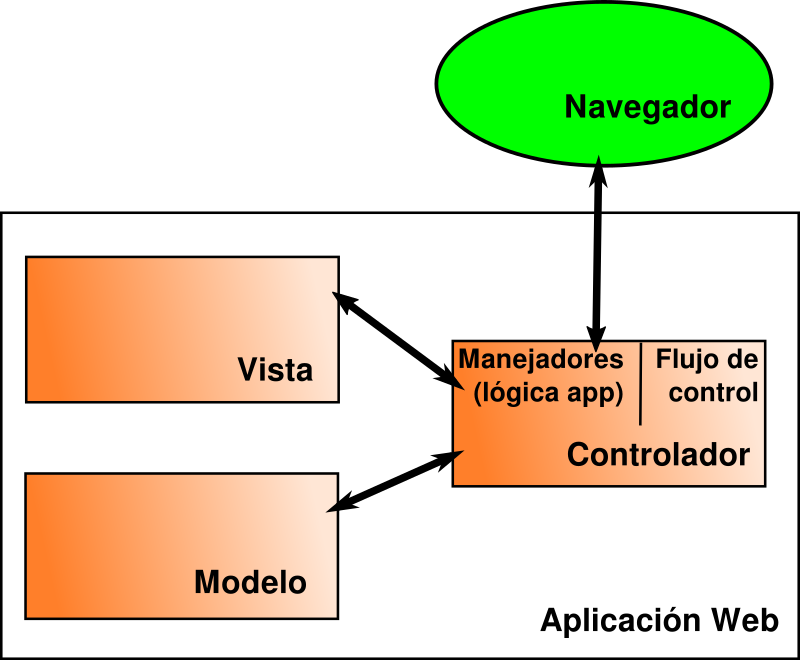
\includegraphics[width=0.8\textwidth]{figs/mvc-basic}
\end{center}
\end{frame}


%%---------------------------------------------------------------

\begin{frame}
\frametitle{MVC en Django}

\begin{itemize}
\item Vista: Manejadores (lógica de aplicación) \\
  funciones en views.py
\item Vistas delegan la presentación en plantillas (templates)
\item Modelo: Descripción de los datos \\
  clases en models.py
\item Controlador: maquinaria de Django \\
  incluyendo urls.py
\item Django como ``plataforma MTV'': \\
  modelo, plantilla (template), vista
\end{itemize}

\end{frame}

%%---------------------------------------------------------------

\begin{frame}
\frametitle{Django: MTV}

\begin{center}
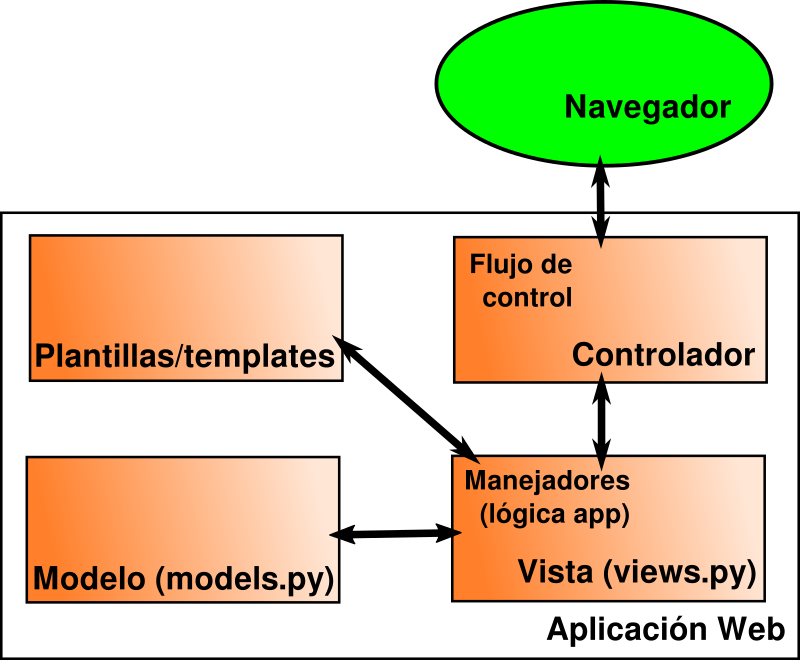
\includegraphics[width=0.8\textwidth]{figs/mvc-mtv}
\end{center}
\end{frame}

%%---------------------------------------------------------------

\begin{frame}
%\frametitle{Django: MTV}

\begin{center}
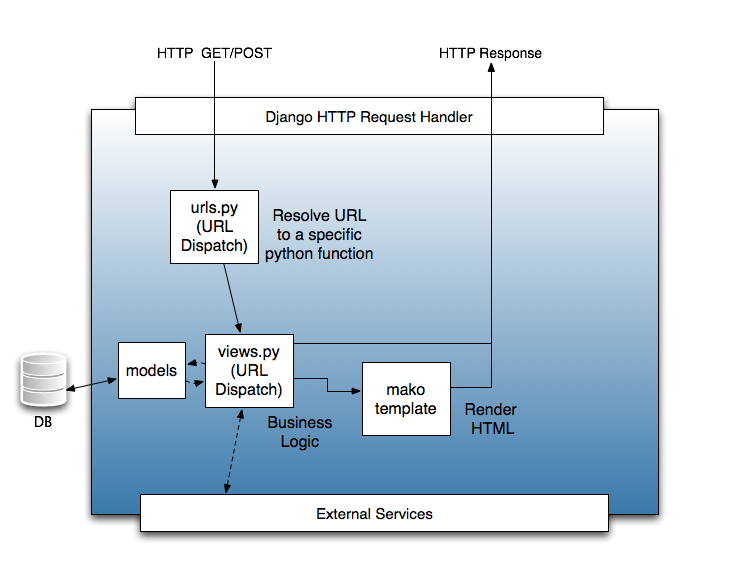
\includegraphics[width=0.85\textwidth]{figs/mvc-mtv-django}
\end{center}

{\footnotesize
Fuente: \url{http://archive.cloudera.com/cdh4/cdh/4/hue/sdk/sdk.html}
}
\end{frame}


%%---------------------------------------------------------------

\begin{frame}
\frametitle{Referencias}

\begin{itemize}
\item MVC, Xerox PARC 1978-79: \\
  \url{http://heim.ifi.uio.no/~trygver/themes/mvc/mvc-index.html}
\item ``The Importance of Model-View Separation. A Conversation with Terence Parr'', by Bill Venners \\
  \url{http://www.artima.com/lejava/articles/stringtemplate.html}
\end{itemize}
\end{frame}

% $Id$
%


\section{Introducci�n a XML}

%%---------------------------------------------------------------

\begin{frame}
\frametitle{Introducci�n}


\begin{itemize}
\item XML: Extensible Markup Language
\item Norma promovida por el W3C (1998)
\item Es un dialecto simplificado de SGML (Standarized General Markup
  Language)
\item Pretende ser razonablemente simple
\item Se est� usando en varios nuevos est�ndares: MathML, SMIL,
  (Synchronized Multimedia Integration Language), DocBook/XML, 
  XHTML, RSS, etc.
\end{itemize}

\end{frame}

%%---------------------------------------------------------------

\begin{frame}[fragile]
\frametitle{Caracter�sticas}

\begin{itemize}
\item Lenguaje de marcado: etiquetas de componentes seg�n su sem�ntica
\item Puede especificarse que un documento ha de estar organizado de
  cierta forma
\item Estructura jer�rquica
\item Sintaxis b�sica:
  \begin{itemize}
  \item Marcas: 
\begin{verbatim}
<p> ... </p> 
<p/>
\end{verbatim}
  \item Atributos: 
\begin{verbatim}
<article lang="es">
\end{verbatim}
  \end{itemize}
\end{itemize}

\end{frame}

%%---------------------------------------------------------------

\begin{frame}[fragile]
\frametitle{Fichero XML sencillo}

\begin{verbatim}
<?xml version="1.0" ?>

<document>
Este es el documento
</document>
\end{verbatim}

\end{frame}

%%---------------------------------------------------------------

\begin{frame}[fragile]
\frametitle{Ejemplo m�s complejo}

Estructura muy simplificada de DocBook:

\begin{verbatim}
<?xml version="1.0" ?>
<article>
  <artheader>
    <title>El lenguaje XML</title>
    <author>Tim Ray</author>
  </artheader>
  <sect1>
    <para>...</para>
  </sect1>
  <sect2>
    <para>...</para>
  </sect2>
</article>
\end{verbatim}

\end{frame}

%%---------------------------------------------------------------

\begin{frame}
\frametitle{Definici�n y validaci�n}

\begin{itemize}
\item XML ofrece la posibilidad de definir lenguajes (tambi�n llamados vocabularios) de etiquetas
\item La definici�n de un lenguaje XML especifica:
  \begin{itemize}
  \item Elementos del lenguaje
  \item Anidamiento de los elementos
  \item Atributos para cada elemento
  \item Atributos por defecto, atributos obligatorios
  \end{itemize}
\item El objetivo es poder validar que un documento XML tiene la informaci�n que se espera y con la estructura correcta.
\end{itemize}

\end{frame}
%%---------------------------------------------------------------

\begin{frame}
\frametitle{Definici�n y validaci�n}

\begin{itemize}
\item Sistemas de definir lenguajes XML
  \begin{itemize}
  \item DTD (Document Type Definition): Est�ndar cl�sico
  \item XML Schema: Nuevo est�ndar. Muy completo y complejo
  \item RelaxNG: Alternativa al nuevo est�ndar. M�s sencillo
  \end{itemize}
\item Cada documento XML debe tener una referencia a su definici�n al principio del fichero (si tiene una)
\end{itemize}

\end{frame}

%%---------------------------------------------------------------

\begin{frame}[fragile]
\frametitle{Ejemplos de lenguajes}

DocBook XML:

\begin{verbatim}
<?xml version="1.0" encoding="ISO-8859-1" ?>
<!DOCTYPE article PUBLIC 
   "-//Norman Walsh//DTD DocBk XML V3.1//EN"
   "/usr/lib/sgml/dtd/docbook-xml/docbookx.dtd">
\end{verbatim}

LaEspiral Document:

\begin{verbatim}
<?xml version="1.0" encoding="ISO-8859-1" ?>
<!DOCTYPE article PUBLIC 
   "-//laespiral.org//DTD LE-document 1.1//EN"
   "http://.../xml/styles/LE-document-1.1.dtd">
\end{verbatim}

\end{frame}

%%---------------------------------------------------------------

\begin{frame}[fragile]
\frametitle{Especificaci�n (ejemplo)}

\begin{verbatim}
<?xml version="1.0" encoding="ISO-8859-1" ?>
<!DOCTYPE joke [
   <!ELEMENT joke (start, end+)>
   <!ATTLIST joke title CDATA #IMPLIED>
   <!ELEMENT start (#PCDATA)>
   <!ELEMENT end (#PCDATA)>
  ]>

<joke title="Van dos''>
  <start>Van dos por una calle</start>
  <end>y se cae el del medio</end>
  <end>y luego vienen</end>
</joke>
\end{verbatim}

\end{frame}

%%---------------------------------------------------------------

\begin{frame}
\frametitle{Bibliotecas para proceso XML}

Tipos de bibliotecas disponibles:

\begin{itemize}
\item DOM
  \begin{itemize}
  \item Document Object Model
  \item Lee todo el documento, y permite recorrer el �rbol de
    elementos
  \item Permite modificar el documento XML
  \end{itemize}
\item SAX
  \begin{itemize}
  \item Standard API for XML
  \item Procesa el documento seg�n est� disponible
  \item Es my r�pido y requiere menos memoria, pero es s�lo para lectura
  \end{itemize}
\item Otras: variantes de DOM y SAX m�s sencillas pero no est�ndar
\end{itemize}

\end{frame}

%%---------------------------------------------------------------

\begin{frame}
\frametitle{Usos t�picos de XML en aplicaciones web}

Gesti�n de interfaz de usuario en navegador:

\begin{itemize}
\item Manipulaci�n de �rbol DOM de la p�gina HTML
\item Realizada normalmente mediante JavaScript
\item Interfaces de usuario mucho m�s ricas
\item Normalmente: combinaci�n con c�digo de aplicaci�n web
\end{itemize}

Intercambio de datos entre aplicaciones web:

\begin{itemize}
\item Fuente para distintos formatos de documento \\
  (ej: documentos en Docbook servidos en HTML, ePub, etc.)
\item Canales (feeds) de una web
\item Interfaz para bases de datos (XPath, etc.)
\item Web sem�ntica (RDF, RDFa)
\end{itemize}
\end{frame}

%%---------------------------------------------------------------

\begin{frame}
\frametitle{DOM de documento HTML en JavaScript (1)}

\begin{itemize}
\item node.parentNode: nodo padre
\item node.childNodes[1]: segundo nodo hijo
\item node.firstChild, x.lastChild: primer, �ltimo nodo hijo
\item document.getElementsByTagName(tag): \\
  vector con todos los elementos con etiqueta tag \\
  $<tag>XXX</tag>$
\item document.getElementById(id): \\
  elemento con identificador id \\
  $<tag id=''id''>XXX</tag>$
\end{itemize}
\end{frame}

%%---------------------------------------------------------------

\begin{frame}
\frametitle{DOM de documento HTML en JavaScript (2)}

\begin{itemize}
\item x.nodeValue: valor del nodo
\item x.innerHTML: HTML que ``cuelga'' del nodo
\item node.setAttribute('attr', val): \\
  asignar a atributo 'attr' a valor val
\item document.createElement(tag) \\
  crear nodo tag
\item document.createTextNode \\
  crear nodo con texto
\item node.appendChild(newnode) \\
  a�ade newnode como hijo de node
\item node.removeChild(remnode) \\
  elimina hijo remnode de node
\end{itemize}

\end{frame}

%%---------------------------------------------------------------

\begin{frame}[fragile]
\frametitle{DOM de documento HTML en JavaScript: ejemplo (1)}

\begin{verbatim}
<html>
  <head>
    <script type="text/javascript" charset="utf-8">
      function change()
      {
      document.getElementById('another').innerHTML =
         'Changed!';
      }
    </script>
  </head>
\end{verbatim}
\end{frame}

%%---------------------------------------------------------------

\begin{frame}[fragile]
\frametitle{DOM de documento HTML en JavaScript: ejemplo (2)}

\begin{verbatim}
<body>
  <h1>Simple DOM demo</h1>
  <p>First sentence</p>
  <p id="sentence">Second sentence, with id "sentence"</p>
  <p id="another">Another sentence, with id "another"</p>
  <p>Text of the sentence with id "sentence":
    <script type="text/javascript" charset="utf-8">
      document.write(
        document.getElementById('sentence').innerHTML
        );
    </script>
  </p>
\end{verbatim}
\end{frame}

%%---------------------------------------------------------------

\begin{frame}[fragile]
\frametitle{DOM de documento HTML en JavaScript: ejemplo (3)}

\begin{verbatim}
    <p>Text of the second sentence:
      <script type="text/javascript" charset="utf-8">
        document.write(
          document.getElementsByTagName('p')[1].innerHTML
          );
      </script>
    </p>
    <form>
      <input type="button" onclick="change()"
        value="Change" />
    </form>
  </body>
</html>
\end{verbatim}
\end{frame}

%%---------------------------------------------------------------

\begin{frame}
\frametitle{Preparaci�n de documentos}

\begin{itemize}
\item Los documentos se escriben en un lenguaje XML (por ejemplo 
   Docbook)
\item Usando hojas de estilo XSL (Extensible Style Language) 
  pueden obtenerse diversos formatos
\item Ventajas
  \begin{itemize}
  \item Ayuda en la estructuraci�n del texto
  \item Simplifica el tratamiento autom�tico
  \item Simplifica la validaci�n
  \item Se separa el contenido de la presentaci�n
  \end{itemize}
\end{itemize}

\end{frame}

%%---------------------------------------------------------------

\begin{frame}
\frametitle{Canales (feeds) de una web}

\begin{itemize}
\item Introducido por Netscape en 1999, para definir ``canales'' (feeds)
\item Permite a los sitios web publicar una lista de las novedades del sitio
\item Esta lista es accedida por aplicaciones lectores de feeds
\item Los usuarios pueden subscribirse a los feeds y recibir avisos de los cambios
\item Lenguajes XML empleados
  \begin{itemize}
  \item RSS 0.91 (Rich Site Summary)
  \item RSS 0.9 y 1.0 (RDF Site Summary)
  \item RSS 2.0 (Really Simple Syndication)
  \item Atom 1.0
  \end{itemize}
\end{itemize}

\end{frame}

%%---------------------------------------------------------------

\begin{frame}[fragile]
\frametitle{Ejemplo de canal RSS (1)}

\begin{verbatim}
<?xml version="1.0" encoding="UTF-8"?>
<rss version="2.0">
<channel>
  <title>Men�ame: publicadas</title>
	
  <link>http://meneame.net</link>
  <image>
    <title>Men�ame: publicadas</title>
    <link>http://meneame.net</link>
    <url>http://meneame.net/img/mnm/eli-rss.png</url>
  </image>
  <description>Sitio colaborativo de publicaci�n y comunicaci�n entre 
   blogs</description>
\end{verbatim}

\end{frame}

%%---------------------------------------------------------------

\begin{frame}[fragile]
\frametitle{Ejemplo de canal RSS (2)}

\begin{verbatim}
  <pubDate>Sat, 22 Nov 2008 13:45:02 +0000</pubDate>
  <item>
    <title>�Qu� pasa cuando un familiar te pide que le montes un 
      PC?</title>
    <link>http://feedproxy.google.com/...-montes-pc</link>
    <pubDate>Sat, 22 Nov 2008 12:55:03 +0000</pubDate>
    <description>&lt;p&gt;Un breve relato que viene a ...
    </description>
  </item>
  <item>...</item>
  <item>...</item>
</channel>
\end{verbatim}

\end{frame}

%%---------------------------------------------------------------

\begin{frame}
\frametitle{Atom}

\begin{itemize}
\item Creado como evoluci�n de RSS 2.0
\item Mejoras que introduce:
  \begin{itemize}
  \item Identificaci�n del tipo de contenido de los elementos summary y content
  \item Incorpora XML namespaces para permitir extender Atom con otros vocabularios XML
  \end{itemize}
\item Mucho m�s apropiado para su interpretaci�n por parte de programas:
  \begin{itemize}
  \item Esto est� provocando su uso habitual en servicios web RESTful
  \end{itemize}
\end{itemize}
\end{frame}

%%---------------------------------------------------------------

\begin{frame}[fragile]
\frametitle{Ejemplo de canal Atom (1)}

\begin{verbatim}
<?xml version="1.0" encoding="utf-8"?>
<feed xmlns="http://www.w3.org/2005/Atom">
    <title>Ejemplo</title>
    <subtitle>Muy interesante</subtitle>
    <link href="http://example.org/"/>
    <updated>2003-12-13T18:30:02Z</updated>
    <author>
       <name>John Doe</name>
       <email>johndoe@example.com</email>
    </author>
    <id>urn:uuid:60a76c80-d399-11d9-b93C-0003939e0af6</id>
\end{verbatim}

\end{frame}

%%---------------------------------------------------------------

\begin{frame}[fragile]
\frametitle{Ejemplo de canal Atom (2)}

\begin{verbatim}
    <entry>
       <title>Atom-Powered Robots Run Amok</title>
       <link href="http://example.org/2003/12/13/atom03"/>
       <id>urn:uuid:1225c695-cfb8-4ebb-aaaa-80da344efa6a</id>
       <updated>2003-12-13T18:30:02Z</updated>
       <summary type="text">Some text.</summary>
    </entry>
</feed>
\end{verbatim}

\end{frame}

%%---------------------------------------------------------------

\begin{frame}[fragile]
\frametitle{Tipos de contenido en Atom}

\begin{verbatim}
 <content type="text">
    Contenido del feed
 </content>
 <content type="html">
    Contenido del &lt;em&gt;feed&lt;/em&gt;
 </content>
 <content type="xhtml" xmlns:xhtml="http://www.w3.org/1999/xhtml">
    <xhtml:div>
      Contenido del <xhtml:em>feed</xhtml:em>
    </xhtml:div>
 </content>
\end{verbatim}

\end{frame}

%%---------------------------------------------------------------

\begin{frame}[fragile]
\frametitle{Web sem�ntica: RDF}

\begin{itemize}
\item RDF: Resource Description Framework
  \begin{itemize}
  \item Mecanismo uniforme para especificar la sem�ntica de un recurso
    web, y su relaci�n con otros.
  \item Cada documento RDF es una serie de tripletes.
  \end{itemize}
\item Modelo de metadatos basado en declaraciones sobre recursos
\item Sujeto (recurso), predicado (relaci�n o aserci�n entre sujeto y
  objeto) y objeto (o valor)
\item Una colecci�n de declaraciones RDF constituyen un grafo
  orientado y etiquetado
\item Es habitual que el recurso sea un URI, el objeto una cadena
  Unicode, y el predicado un URI
\end{itemize}

\end{frame}

%%---------------------------------------------------------------

\begin{frame}
\frametitle{Otras tecnolog�as de la familia XML}

\begin{itemize}
\item XLink: enlaces entre documentos XML
\item XSLT: conversi�n autom�tica de XML a otros formatos
\item XPath: localizaci�n dentro de un documento (``query'' sobre XML)

\end{itemize}
\end{frame}

%%---------------------------------------------------------------

\begin{frame}
\frametitle{XML Namespaces}

\begin{itemize}
\item Permiten agrupar varios vocabularios XML en un �nico documento
\item Resuelven el problema de colisiones entre etiquetas con el mismo nombre
\end{itemize}

\end{frame}

%%---------------------------------------------------------------

\begin{frame}
\frametitle{Ejemplo: Problema}

Introducir en el canal de una web informaci�n geogr�fica
\begin{itemize}
\item Existen dos lenguajes XML distintos para cada informaci�n:
  \begin{itemize}
  \item RSS o Atom: Permiten dar informaci�n del canal y sus items
  \item geoRSS: Permite especificar longitud y latitud
  \end{itemize}
\end{itemize}

\end{frame}

%%---------------------------------------------------------------

\begin{frame}[fragile]
\frametitle{Ejemplo: Soluci�n}

\begin{verbatim}
<rss xmlns:georss="http://www.georss.org/georss" 
     version="2.0">
<channel>
  <item>
    <title>En M�laga colocar publicidad en los parabrisas de
     los coches se multar� con hasta 750 euros</title>
     <georss:point>36.7196745 -4.4200359</georss:point>
     ...
\end{verbatim}

\end{frame}

%%---------------------------------------------------------------

\begin{frame}
\frametitle{Uso de Namespaces en la pr�ctica}

\begin{itemize}
\item El parser empleado debe soportar namespaces: la mayor�a lo hacen ya
\item Problema: el mecanismo de validaci�n original de XML, los DTDs, no 
  proporciona ninguna soluci�n para validar documentos XML con namespaces
  \begin{itemize}
  \item Soluci�n: usar XML Schema o RelaxNG
  \end{itemize}
\end{itemize}
\end{frame}


%%---------------------------------------------------------------

\begin{frame}
\frametitle{Alternativa a XML: JSON}

\begin{itemize}
\item JavaScript Object Notation
\item Definido en RFC 4627
\item Internet media type: application/json.
\item Permite representar estructuras de datos
\item Espec�ficamente pensado para aplicaciones AJAX
\item Es un subconjunto de JavaScript (y de Python)
\end{itemize}
\end{frame}

%%---------------------------------------------------------------

\begin{frame}[fragile]
\frametitle{Ejemplo de JSON}

\begin{verbatim}
{
    "firstName": "John",
    "lastName": "Smith",
    "address": {
        "streetAddress": "21 2nd Street",
        "city": "New York",
        "state": "NY",
        "postalCode": 10021
    },
    "phoneNumbers": [
        "212 732-1234",
        "646 123-4567"
    ]
}
\end{verbatim}

\end{frame}

%%---------------------------------------------------------------

\begin{frame}
\frametitle{Uso en la pr�ctica de JSON}

Existen int�rpretes para casi cualquier lenguaje:
\begin{itemize}
\item JavaScript: La funci�n eval() es capaz de int�rpretarlo directamente. \\
  Pero mejor usar el m�dulo JSON
\item Python: m�dulo json
\item Java: JSON Tools, xstream, Restlet, ...
\item   ...
\end{itemize}

Extensiones:
\begin{itemize}
\item JSONT: Equivalente a XSLT para JSON
\item JSONP: convierte el contenido en activo al incluir la invocaci�n a una funci�n JavaScript.
\end{itemize}
\end{frame}


%%---------------------------------------------------------------

\begin{frame}
\frametitle{Ventajas e Inconvenientes}

Ventajas
\begin{itemize}
\item Requiere menos caractereres para la misma informaci�n (consume menos ancho de banda)
\item Es f�cil escribir un int�rprete r�pido (incluso en un navegador)
\item F�cil de leer por personas
\end{itemize}

Inconvenientes
\begin{itemize}
\item No tiene mecanismos de definici�n de lenguajes y validaci�n
\item No hay equivalentes a Atom, XSLT, ...
\end{itemize}
\end{frame}

  
%%---------------------------------------------------------------

\begin{frame}
\frametitle{Referencias}

\begin{itemize}
\item Introducci�n al XML, por Jaime Villate: \\
  \url{http://gsyc.escet.urjc.es/actividades/linuxprog/xml/xml-notas.html}
\item Especificaci�n de XML: \\
  \url{http://www.w3.org/TR/xml-spec.html}
\item Especificaci�n anotada de XML: \\
  \url{http://www.xml.com/xml/pub/axml/axmlintro.html}
\item Python and XML Processing: \\
  \url{http://pyxml.sourceforge.net/topics/}
\item SIG for XML Processing in Python: \\
  \url{http://www.python.org/sigs/xml-sig/}
\end{itemize}
\end{frame}

%%---------------------------------------------------------------

\begin{frame}
\frametitle{Referencias II}

\begin{itemize}
\item Python/XML HOWTO: \\
  \url{http://py-howto.sourceforge.net/xml-howto/}
\item XML Linking Language (XLink): \\
  \url{http://www.w3.org/TR/xlink/}
\item XML Path Language (XPath): \\
  \url{http://www.w3.org/TR/xpath}
\item XPath Tutorial, por Miloslav Nic y Jiri Jirat: \\
  \url{http://www.zvon.org/xxl/XPathTutorial/General/examples.html}
\item XML Schema: \\
  \url{http://www.w3.org/XML/Schema}
\end{itemize}
\end{frame}

%%---------------------------------------------------------------

\begin{frame}
\frametitle{Referencias III}

\begin{itemize}
\item Using W3C XML Schema, por  Eric van der Vlist: \\
  \url{http://www.xml.com/pub/a/2000/11/29/schemas/part1.html}
\item XSL Transformations (XSLT): \\
  \url{http://www.w3.org/TR/xslt}
\item P�gina DOM del W3C: \\
  \url{http://www.w3.org/DOM/}
\item P�gina de SAX:
  \url{http://www.megginson.com/SAX/}
\item P�gina de RDF:
  \url{http://www.w3.org/RDF/}
\item RSS 1.0: \\
  \url{http://groups.yahoo.com/group/rss-dev/files/specification.html}
\end{itemize}
\end{frame}

%%---------------------------------------------------------------

\begin{frame}
\frametitle{Referencias IV}

\begin{itemize}
\item XML Namespaces: \\
  \url{http://www.w3.org/TR/REC-xml-names/}
\item XML Schema: \\
  \url{http://www.w3.org/XML/Schema}
\item Relax NG: \\
  \url{http://relaxng.org}
\item Atom (RFC4287): \\
  \url{http://tools.ietf.org/html/rfc4287}
\item W3C DOM -Introduction: \\
  \url{http://www.quirksmode.org/dom/intro.html}
\item JSON: \\
  \url{http://json.org/}
\end{itemize}
\end{frame}

\include{www-novedades}
% $Id$
%

\section{Hojas de estilo CSS}


%%---------------------------------------------------------------

\begin{frame}
\frametitle{�Qu� es CSS?}

\begin{itemize}
  \item Es un lenguaje de hojas de estilos creado para {\bf controlar el aspecto} o presentaci�n de los documentos electr�nicos definidos con HTML
  \item Es la mejor forma de {\bf separar los contenidos y su presentaci�n} y es imprescindible para crear p�ginas web complejas
  \begin{itemize}
    \item Obliga a crear documentos HTML bien definidos y con significado completo (tambi�n llamados \emph{documentos sem�nticos})
    \item Mejora la accesibilidad del documento
    \item Reduce la complejidad de su mantenimiento
    \item Permite visualizar el mismo documento en infinidad de dispositivos diferentes
  \end{itemize}
\end{itemize}

\end{frame}

%%---------------------------------------------------------------

\begin{frame}[fragile]
\frametitle{Antes del CSS}

{\footnotesize
\begin{verbatim}
<!DOCTYPE html>
<html>
<head>
 <meta http-equiv="Content-Type" content="text/html; charset=iso-8859-1"/>
 <title>Ejemplo de estilos sin CSS</title>
</head>
 
<body>
 <h1><font color="red" face="Arial" size="5">
    Titular de la p�gina
 </font></h1>
 <p><font color="gray" face="Verdana" size="2">
   Un p�rrafo de texto no muy largo.
 </font></p>
</body>
</html>
\end{verbatim}
}

\end{frame}

%%---------------------------------------------------------------

\begin{frame}[fragile]
\frametitle{Con CSS}

{\footnotesize
\begin{verbatim}
<!DOCTYPE html">
<html>
<head>
<meta http-equiv="Content-Type" content="text/html; charset=iso-8859-1"/>
<title>Ejemplo de estilos con CSS</title>
<style type="text/css">
  h1 { color: red;  font-family: Arial;   font-size: large;  }
  p  { color: gray; font-family: Verdana; font-size: medium; }
</style>
</head>
 
<body>
  <h1>Titular de la p�gina</h1>
  <p>Un p�rrafo de texto no muy largo.</p>
</body>
</html>
\end{verbatim}
}

\end{frame}

%%---------------------------------------------------------------

\begin{frame}
\frametitle{CSS en un documento HTML}

Se pueden integrar instrucciones CSS de varias maneras en un documento
HTML:

\begin{enumerate}
  \item Incluir CSS en el mismo documento HTML
  \item Definir CSS en un archivo externo
  \item Incluir CSS en los elementos HTML
\end{enumerate}

\end{frame}

%%---------------------------------------------------------------

\begin{frame}
\frametitle{Glosario B�sico (I)}

\begin{center}
\begin{figure}[p]
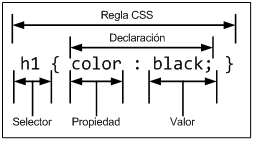
\includegraphics[width=0.6\textwidth]{figs/f0101.png}
\end{figure}
\end{center}

\begin{itemize}
  \item {\bf Regla}: cada uno de los estilos que componen una hoja de estilos CSS. Cada regla est� compuesta de una parte de ``selectores'', un s�mbolo de ``llave de apertura'' (\{), otra parte denominada ``declaraci�n'' y por �ltimo, un s�mbolo de ``llave de cierre'' (\}).
  \item {\bf Selector}: indica el elemento o elementos HTML a los que se aplica la regla CSS.
\end{itemize}

\end{frame}

%%---------------------------------------------------------------

\begin{frame}
\frametitle{Glosario B�sico (y II)}

\begin{center}
\begin{figure}[p]
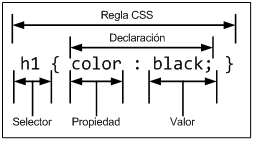
\includegraphics[width=0.42\textwidth]{figs/f0101.png}
\end{figure}
\end{center}

\begin{itemize}
  \item {\bf Declaraci�n}: especifica los estilos que se aplican a los elementos. Est� compuesta por una o m�s propiedades CSS.
  \item {\bf Propiedad}: caracter�stica que se modifica en el elemento seleccionado, como por ejemplo su tama�o de letra, su color de fondo, etc.
  \item {\bf Valor}: establece el nuevo valor de la caracter�stica modificada en el elemento.
\end{itemize}

CSS 2.1 define 115 propiedades, mientras que CSS 3 define 239 propiedades.

\end{frame}

%%---------------------------------------------------------------
%
%\begin{frame}
%\frametitle{Sintaxis}
%
%\begin{itemize}
%  \item Sucesi�n de palabras sin ning�n car�cter que las separe (par�ntesis, comas, barras, etc.) el valor de la propiedad se debe indicar tal y como se muestra y con esas palabras en el mismo orden.
%  \item Sucesi�n de valores separados por una barra simple el valor de la propiedad debe tomar uno y s�lo uno de los valores indicados
%  \item Sucesi�n de valores separados por una barra doble el valor de la propiedad puede tomar uno o m�s valores de los indicados y en cualquier orden.
%  \item Cada valor o agrupaci�n de valores se puede indicar el tipo de valor: opcional, obligatorio, m�ltiple o restringido.
%  \item M�s: * = cero o m�s veces; + = una o m�s veces; ? = opcional; {n1, n2} = entre n1 y n2 veces
%\end{itemize}
%
%\end{frame}


%%---------------------------------------------------------------

\subsubsection*{Selectores}

\begin{frame}
\frametitle{Selectores}

\begin{itemize}
  \item A un mismo elemento HTML se le pueden aplicar varias reglas 
  \item Cada regla puede aplicarse a un n�mero ilimitado de elementos
  \item Cuando el selector de dos o m�s reglas CSS es id�ntico, se pueden agrupar las declaraciones de las reglas para hacer las hojas de estilos m�s eficientes
  \item Cuando se establece el valor de una propiedad CSS en un elemento, sus elementos descendientes heredan de forma autom�tica el valor de esa propiedad
\end{itemize}

CSS 2.1 incluye una docena de tipos diferentes de selectores, que permiten seleccionar de forma muy precisa elementos individuales o conjuntos de elementos dentro de una p�gina web.

\end{frame}

%%---------------------------------------------------------------

\begin{frame}
\frametitle{Selectores b�sicos}

\begin{enumerate}
  \item Selector universal
  \item Selector de tipo o etiqueta
  \item Selector descendente
  \item Selector de clase
  \item Selector de identidad
\end{enumerate}

\end{frame}

%%---------------------------------------------------------------

\begin{frame}[fragile]
\frametitle{Selector Universal}

\begin{itemize}
  \item No se utiliza habitualmente
  \item Generalmente es equivalente para poner estilo a $<body>$
  \item Se suele combinar con otros selectores y adem�s, forma parte de algunos hacks muy utilizados
\end{itemize}

\begin{verbatim}
* {
  margin: 0;
  padding: 0;
}
\end{verbatim}

\end{frame}

%%---------------------------------------------------------------

\begin{frame}[fragile]
\frametitle{Selector de tipo o etiqueta}

\begin{itemize}
  \item Selecciona todos los elementos de la p�gina cuya etiqueta HTML coincide con el valor del selector
  \item Se pueden agrupar todas las reglas individuales en una sola regla con un selector m�ltiple.
  \item Buena pr�ctica: agrupar las propiedades comunes de varios elementos en una �nica regla CSS y posteriormente definir las propiedades espec�ficas de esos mismos elementos
\end{itemize}

{\footnotesize
\begin{verbatim}
h1, h2, h3 {
  color: #8A8E27;
  font-weight: normal;
  font-family: Arial, Helvetica, sans-serif;
}
 
h1 { font-size: 2em; }
h2 { font-size: 1.5em; }
h3 { font-size: 1.2em; }
\end{verbatim}
}

\end{frame}

%%---------------------------------------------------------------

\begin{frame}[fragile]
\frametitle{Selector descendente}

\begin{itemize}
  \item Selecciona los elementos que se encuentran dentro de otros elementos. Un elemento es descendiente de otro cuando se encuentra entre las etiquetas de apertura y de cierre del otro elemento.
\end{itemize}

\begin{verbatim}
p span { color: red; }
[...]
<p>
  ...
  <span>texto1</span>
  ...
  <a href="">...<span>texto2</span></a>
  ...
</p>
\end{verbatim}

Al resto de elementos $<span>$ de la p�gina que no est�n dentro de un elemento $<p>$, no se les aplica la regla CSS anterior.

\end{frame}

%%---------------------------------------------------------------

\begin{frame}
\frametitle{Ejercicio}

�Qu� elementos se seleccionar�an con estos tipos de selectores?

\begin{itemize}
  \item p a span em \{ text-decoration: underline; \}
  \item p, a, span, em \{ text-decoration: underline; \}
  \item p a \{ color: red; \}
  \item p * a \{ color: red; \}
\end{itemize}

\end{frame}

%%---------------------------------------------------------------

\begin{frame}[fragile]
\frametitle{Selector de clase}

\begin{itemize}
  \item Se utiliza el atributo class de HTML sobre ese elemento para indicar directamente la regla CSS que se le debe aplicar
  \item Se crea en el archivo CSS una nueva regla llamada destacado con todos los estilos que se van a aplicar al elemento
  \item Se prefija el valor del atributo class con un punto (.)
\end{itemize}

{\footnotesize
\begin{verbatim}
.destacado { color: red; }
[...]
  <p class="destacado">Lorem ipsum dolor sit amet...</p>
  <p>Nunc sed lacus et 
<a href="#" class="destacado">est adipiscing</a>
  accumsan...</p>
  <p>Class aptent taciti <em class="destacado">sociosqu
ad</em> litora...</p>
\end{verbatim}
}

\end{frame}

%%---------------------------------------------------------------

\begin{frame}[fragile]
\frametitle{Selector de clase m�s espec�fico}

\begin{itemize}
  \item Combinando el selector de tipo y el selector de clase, se obtiene un selector mucho m�s espec�fico.
\end{itemize}

{\footnotesize
\begin{verbatim}
p.destacado { color: red }
[...]
  <p class="destacado">Lorem ipsum dolor sit amet...</p>
  <p>Nunc sed lacus et <a href="#" class="destacado">est
adipiscing</a> accumsan...</p>
  <p>Class aptent taciti <em class="destacado">sociosqu
ad</em> litora...</p>
\end{verbatim}
}

\end{frame}

%%---------------------------------------------------------------

\begin{frame}
\frametitle{Ejercicio}

�Qu� elementos se seleccionar�an con estos tipos de selectores?

\begin{itemize}
  \item p.aviso \{ ... \}
  \item p .aviso \{ ... \}
  \item p, .aviso \{ ... \}
  \item *.aviso \{ ... \}
\end{itemize}

\end{frame}

%%---------------------------------------------------------------

\begin{frame}[fragile]
\frametitle{Selectores de identificador}

\begin{itemize}
  \item Aplica estilos CSS a un �nico elemento de la p�gina
  \item El valor del atributo id no se puede repetir en dos elementos diferentes de una misma p�gina
\end{itemize}

\begin{verbatim}
#destacado { color: red; }
 
<p>Primer p�rrafo</p>
<p id="destacado">Segundo p�rrafo</p>
<p>Tercer p�rrafo</p>
\end{verbatim}

\end{frame}


%%---------------------------------------------------------------

\begin{frame}
\frametitle{Ejercicio}

�Qu� elementos se seleccionar�an con estos tipos de selectores?

\begin{itemize}
  \item p\#aviso \{ ... \}
  \item p \#aviso \{ ... \}
  \item p, \#aviso \{ ... \}
  \item *\#aviso \{ ... \}
\end{itemize}

�Tienen sentido estos selectores? �Cu�ndo?

\end{frame}

%%---------------------------------------------------------------

\begin{frame}
\frametitle{Ejercicio: Combinaci�n de selectores}

�Qu� elementos se seleccionar�an con estos tipos de selectores?

\begin{itemize}
  \item .aviso .especial \{ ... \}
  \item div.aviso span.especial \{ ... \}
  \item ul\#menuPrincipal li.destacado a\#inicio \{ ... \}
\end{itemize}

\end{frame}

%%---------------------------------------------------------------

\begin{frame}
\frametitle{Colisi�n de estilos (simplificado)}

\begin{enumerate}
  \item Cuanto m�s espec�fico sea un selector, m�s importancia tiene su regla asociada.
  \item A igual especificidad, se considera la �ltima regla indicada.
\end{enumerate}

\end{frame}



%%---------------------------------------------------------------

\subsubsection*{Unidades y colores}

\begin{frame}
\frametitle{Unidades de medida}

\begin{itemize}
  \item Unidades absolutas
  \begin{itemize}
    \item in, cm, mm, pt, pc
  \end{itemize}
  \item Unidades relativas
  \begin{itemize}
    \item em, ex, px
  \end{itemize}
  \item Porcentajes
\end{itemize}

En general, se recomienda el uso de unidades relativas siempre que sea posible

Normalmente se utilizan p�xel y porcentajes para definir el layout del documento (b�sicamente, la anchura de las columnas y de los elementos de las p�ginas) y em y porcentajes para el tama�o de letra de los textos.

\end{frame}

%%---------------------------------------------------------------

\begin{frame}
\frametitle{Colores}

\begin{itemize}
  \item Palabras clave
  \begin{itemize}
    \item aqua, black, blue, fuchsia, gray...
  \end{itemize}
  \item RGB decimal
  \item RGB porcentual
  \item RGB hexadecimal
\end{itemize}

\end{frame}


%%---------------------------------------------------------------

\begin{frame}
\frametitle{Tipos de elementos (I)}

El est�ndar HTML clasifica a todos sus elementos en dos grandes grupos:

Elementos de l�nea:

\begin{itemize}
  \item Los elementos en l�nea (``inline elements'' en ingl�s) no empiezan necesariamente en nueva l�nea y s�lo ocupan el espacio necesario para mostrar sus contenidos.

\end{itemize}

\end{frame}

%%---------------------------------------------------------------

\begin{frame}
\frametitle{Tipos de elementos (II)}

Elementos de bloque:

\begin{itemize}
  \item Los elementos de bloque (``block elements'' en ingl�s) siempre empiezan en una nueva l�nea y ocupan todo el espacio disponible hasta el final de la l�nea
\end{itemize}

\begin{center}
\begin{figure}[p]
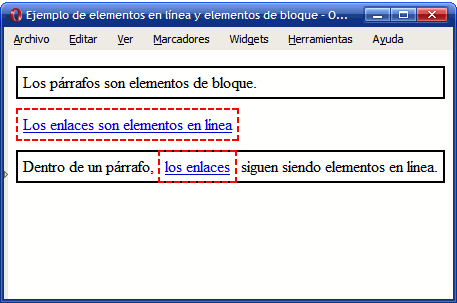
\includegraphics[width=0.8\textwidth]{figs/f0501.png}
\end{figure}
\end{center}

Por sus caracter�sticas, los elementos de bloque no pueden insertarse dentro de elementos en l�nea y tan s�lo pueden aparecer dentro de otros elementos de bloque. En cambio, un elemento en l�nea puede aparecer tanto dentro de un elemento de bloque como dentro de otro elemento en l�nea.

\end{frame}



%%---------------------------------------------------------------

\subsubsection*{El Modelo de Cajas}

\begin{frame}
\frametitle{El modelo de cajas}

\begin{itemize}
  \item Es el comportamiento de CSS que hace que todos los elementos de las p�ginas se representen mediante cajas rectangulares
  \item  Cada vez que se inserta una etiqueta HTML, se crea una nueva caja rectangular que encierra los contenidos de ese elemento
\end{itemize}


\begin{center}
\begin{figure}[p]
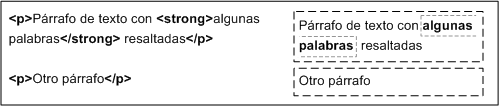
\includegraphics[width=0.8\textwidth]{figs/f0402.png}
\end{figure}
\end{center}

\end{frame}

%%---------------------------------------------------------------

\begin{frame}
\frametitle{El modelo de cajas (II)}

\begin{itemize}
  \item No son visibles a simple vista porque inicialmente no muestran ning�n color de fondo ni ning�n borde
\end{itemize}

\begin{center}
\begin{figure}[p]
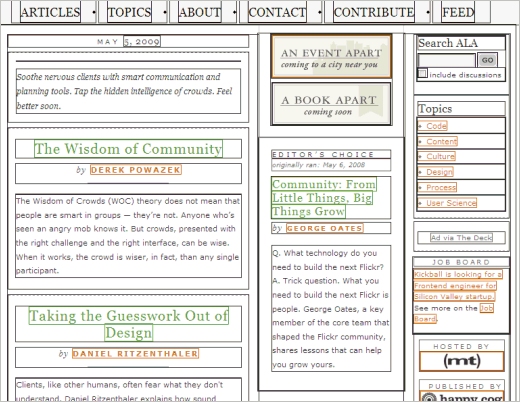
\includegraphics[width=0.55\textwidth]{figs/f0401.png}
\end{figure}
\end{center}
{\footnotesize
Ejemplo de http://www.alistapart.com/ despu�s de forzar a que todas las cajas muestren su borde
}

\end{frame}

%%---------------------------------------------------------------

\begin{frame}
\frametitle{El modelo de cajas (III)}

\begin{itemize}
  \item Los navegadores crean y colocan las cajas de forma autom�tica, pero CSS permite modificar todas sus caracter�sticas. Cada una de las cajas est� formada por seis partes, tal y como muestra la siguiente imagen:
\end{itemize}


\begin{center}
\begin{figure}[p]
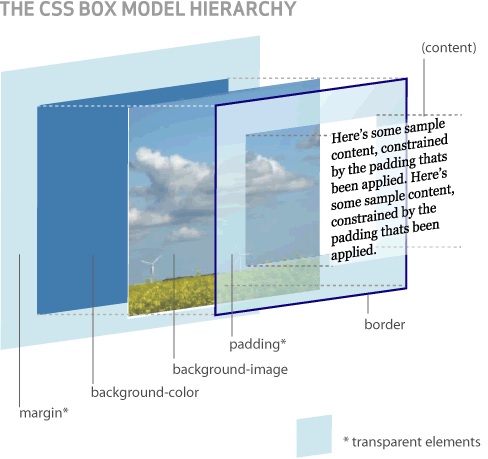
\includegraphics[width=0.45\textwidth]{figs/f0403.png}
\end{figure}
\end{center}
{\footnotesize
 Representaci�n tridimensional del box model de CSS
(Esquema utilizado con permiso de http://www.hicksdesign.co.uk/boxmodel/)
}
\end{frame}

%%---------------------------------------------------------------

\begin{frame}
\frametitle{Partes que componen cada caja}

\begin{itemize}
  \item {\bf Contenido} (content): se trata del contenido HTML del elemento (las palabras de un p�rrafo, una imagen, el texto de una lista de elementos, etc.)
  \item {\bf Relleno} (padding): espacio libre opcional existente entre el contenido y el borde.
  \item {\bf Borde} (border): l�nea que encierra completamente el contenido y su relleno.
  \item {\bf Imagen de fondo} (background image): imagen que se muestra por detr�s del contenido y el espacio de relleno.
  \item {\bf Color de fondo} (background color): color que se muestra por detr�s del contenido y el espacio de relleno.
  \item {\bf Margen} (margin): separaci�n opcional existente entre la caja y el resto de cajas adyacentes.
\end{itemize}

\end{frame}


%%---------------------------------------------------------------

\begin{frame}[fragile]
\frametitle{Margen, relleno, bordes y modelo de cajas (I)}

\begin{itemize}
  \item El margen, el relleno y los bordes establecidos a un elemento determinan la anchura y altura final del elemento
\end{itemize}

{\footnotesize
\begin{verbatim}
div {
  width: 300px;
  padding-left:  50px;
  padding-right: 50px;
  margin-left:   30px;
  margin-right:  30px;
  border: 10px solid black;
}
\end{verbatim}
}



\end{frame}

%%---------------------------------------------------------------

\begin{frame}[fragile]
\frametitle{Margen, relleno, bordes y modelo de cajas (y II)}

\begin{center}
\begin{figure}[p]
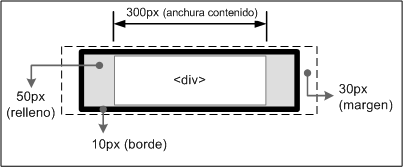
\includegraphics[width=0.75\textwidth]{figs/f0414.png}
\end{figure}
\end{center}

De esta forma, la anchura del elemento en pantalla ser�a igual a la suma de la anchura original, los m�rgenes, los bordes y los rellenos:

30px + 10px + 50px + 300px + 50px + 10px + 30px = 480 p�xel

\end{frame}

%%---------------------------------------------------------------

\begin{frame}
\frametitle{Visualizaci�n}

\begin{itemize}
  \item CSS define otras cuatro propiedades para controlar su visualizaci�n: display, visibility, overflow y z-index.
  \item La propiedad display permite ocultar completamente un elemento haciendo que desaparezca de la p�gina. Como el elemento oculto no se muestra, el resto de elementos de la p�gina se mueven para ocupar su lugar.
  \item La propiedad display tambi�n permite modificar el comportamiento de un elemento a bloque (block) o en l�nea (inline).
  \item La propiedad visibility permite hacer invisible un elemento, lo que significa que el navegador crea la caja del elemento pero no la muestra. En este caso, el resto de elementos de la p�gina no modifican su posici�n, ya que aunque la caja no se ve, sigue ocupando sitio.
\end{itemize}

\end{frame}


%%---------------------------------------------------------------

\begin{frame}
\frametitle{Diferencias entre display y visibility}

\begin{center}
\begin{figure}[p]
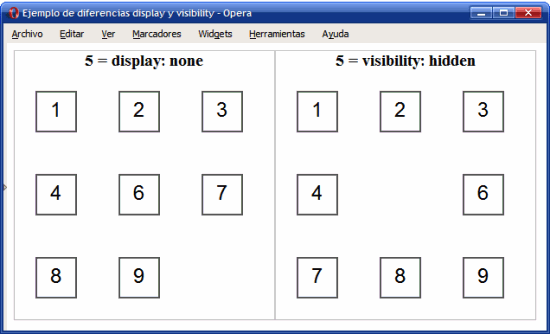
\includegraphics[width=0.8\textwidth]{figs/f0522.png}
\end{figure}
\end{center}

\end{frame}



%%---------------------------------------------------------------

\begin{frame}
\frametitle{Propiedades margin}

\begin{center}
  \begin{table}
   \begin{tabular}{p{1.8cm}p{7.8cm}}
Propiedades &\bf{margin-top}, \bf{margin-right}, \bf{margin-bottom}, \bf{margin-left} \\ \hline
Valores & $<medida>$ | $<porcentaje>$ | auto | inherit \\ \hline
Se aplica a & Todos los elementos, salvo margin-top y margin-bottom que s�lo se aplican a los elementos de bloque y a las im�genes \\ \hline
Valor inicial & 0 \\ \hline
Descripci�n & Establece cada uno de los m�rgenes horizontales y verticales de un elemento \\  \hline
  \end{tabular}
    \caption{Definici�n de la propiedad \emph{margin-top}, \emph{margin-right}, \emph{margin-bottom}, \emph{margin-left} de CSS}
 \end{table}
\end{center}

\end{frame}

%%---------------------------------------------------------------

\begin{frame}
\frametitle{Propiedad margin (propiedad \emph{shorthand})}

\begin{center}
  \begin{table}
   \begin{tabular}{p{1.8cm}p{7.8cm}}
Propiedad &\bf{margin} \\ \hline
Valores & ( $<medida>$ | $<porcentaje>$ | auto ) {1, 4} | inherit \\ \hline
Se aplica a & Todos los elementos salvo algunos casos especiales de elementos mostrados como tablas \\ \hline
Valor inicial & - \\ \hline
Descripci�n & Establece de forma directa todos los m�rgenes de un elemento \\ \hline
 \end{tabular}
   \caption{Definici�n de la propiedad margin de CSS}
 \end{table}
\end{center}

\end{frame}

%%---------------------------------------------------------------

\begin{frame}
\frametitle{Propiedad margin (propiedad \emph{shorthand}) (y II)}

La notaci�n {1, 4} de la definici�n anterior significa que la propiedad margin admite entre uno y cuatro valores, con el siguiente significado:

\begin{itemize}
  \item Si solo se indica un valor, todos los m�rgenes tienen ese valor.
  \item Si se indican dos valores, el primero se asigna al margen superior e inferior y el segundo se asigna a los m�rgenes izquierdo y derecho.
  \item Si se indican tres valores, el primero se asigna al margen superior, el tercero se asigna al margen inferior y el segundo valor se asigna los m�rgenes izquierdo y derecho.
  \item Si se indican los cuatro valores, el orden de asignaci�n es: margen superior, margen derecho, margen inferior y margen izquierdo.
\end{itemize}

\end{frame}


\begin{frame}
\frametitle{Posicionamiento y visualizaci�n}

\begin{itemize}
  \item Los navegadores crean y posicionan de forma autom�tica todas las cajas que forman cada p�gina HTML
  \item El dise�ador puede modificar la posici�n en la que se muestra cada caja.
  \item Existen {\bf cuatro tipos de posicionamiento} definidos para las cajas
\end{itemize}

\end{frame}



%%---------------------------------------------------------------

\begin{frame}
\frametitle{Tipos de posicionamiento}

\begin{itemize}
  \item {\bf Normal o est�tico}: posicionamientosi no se indica lo contrario.
  \item{\bf Relativo}: consiste en posicionar una caja seg�n el posicionamiento normal y despu�s desplazarla respecto de su posici�n original.
  \item {\bf Absoluto}: la posici�n de una caja se establece de forma absoluta respecto de su elemento contenedor y el resto de elementos de la p�gina ignoran la nueva posici�n del elemento.
  \item {\bf Fijo}: variante del posicionamiento absoluto que convierte una caja en un elemento inamovible, de forma que su posici�n en la pantalla siempre es la misma independientemente del resto de elementos e independientemente de si el usuario sube o baja la p�gina en la ventana del navegador.
  \item {\bf Flotante}: desplaza las cajas todo lo posible hacia la izquierda o hacia la derecha de la l�nea en la que se encuentran.
\end{itemize}

\end{frame}

%%---------------------------------------------------------------
\subsubsection*{Enlaces}

\begin{frame}
\frametitle{Pseudo-clases}

Como con los atributos id o class no es posible aplicar diferentes estilos a un mismo elemento en funci�n de su estado, CSS introduce un nuevo concepto llamado pseudo-clases. En enlaces:

\begin{itemize}
  \item {\bf :link}: enlaces que apuntan a p�ginas o recursos que a�n no han sido visitados por el usuario.
  \item {\bf :visited}: enlaces que apuntan a recursos que han sido visitados anteriormente por el usuario. El historial de enlaces visitados se borra autom�ticamente cada cierto tiempo y el usuario tambi�n puede borrarlo manualmente.
  \item {\bf :hover}: enlace sobre el que el usuario ha posicionado el puntero del rat�n.
  \item {\bf :active}: enlace que est� pinchando el usuario. Los estilos s�lo se aplican desde que el usuario pincha el bot�n del rat�n hasta que lo suelta.
\end{itemize}

\end{frame}


%%---------------------------------------------------------------

\begin{frame}
\frametitle{Im�genes seg�n el estilo del enlace}

\begin{itemize}
  \item En ocasiones, puede resultar �til incluir un peque�o icono al lado de un enlace para indicar el tipo de contenido que enlaza.
  \item Este tipo de im�genes son puramente decorativas en vez de im�genes de contenido, por lo que se deber�an a�adir con CSS y no con elementos de tipo $<img>$. Utilizando la propiedad background (y background-image) se puede personalizar el aspecto de los enlaces para que incluyan un peque�o icono a su lado.
  \item La t�cnica consiste en mostrar una imagen de fondo sin repetici�n en el enlace y a�adir el padding necesario al texto del enlace para que no se solape con la imagen de fondo.
\end{itemize}

\end{frame}


%%---------------------------------------------------------------

\begin{frame}[fragile]
\frametitle{Im�genes seg�n el estilo del enlace (II)}

\begin{footnotesize}
\begin{verbatim}
a { margin: 1em 0; float: left; clear: left; }
 
.rss {
  color: #E37529;
  padding: 0 0 0 18px;
  background: #FFF url(imagenes/rss.gif) no-repeat left center;
}
 
.pdf {
  padding: 0 0 0 22px;
  background: #FFF url(imagenes/pdf.png) no-repeat left center;
}
 
<a href="#">Enlace con el estilo por defecto</a>
<a class="rss" href="#">Enlace a un archivo RSS</a>
<a class="pdf" href="#">Enlace a un documento PDF</a>
\end{verbatim}
\end{footnotesize}

\end{frame}

%%---------------------------------------------------------------

\begin{frame}
\frametitle{Im�genes seg�n el estilo del enlace (y III)}


\begin{center}
\begin{figure}[p]
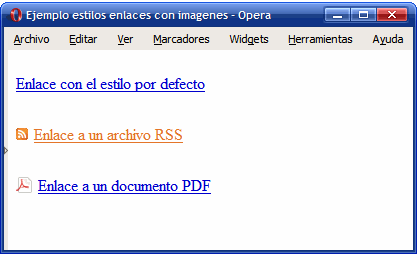
\includegraphics[width=0.8\textwidth]{figs/f0704.png}
\end{figure}
\end{center}

\end{frame}


%%---------------------------------------------------------------

\begin{frame}[fragile]
\frametitle{Mostrar los enlaces como si fueran botones}

\begin{footnotesize}
\begin{verbatim}
a { margin: 1em 0; float: left; clear: left; }
a.boton {
  text-decoration: none;
  background: #EEE;
  color: #222;
  border: 1px outset #CCC;
  padding: .1em .5em;
}
a.boton:hover {
  background: #CCB;
}
a.boton:active {
  border: 1px inset #000;
}
<a class="boton" href="#">Guardar</a>
<a class="boton" href="#">Enviar</a>
\end{verbatim}
\end{footnotesize}

\end{frame}



%%---------------------------------------------------------------

\begin{frame}
\frametitle{Crear un men� vertical}

\begin{enumerate}
  \item Definir anchura del men�
  \item Eliminar las vi�etas autom�ticas y todos los m�rgenes y espaciados aplicados por defecto
  \item A�adir un borde al men� de navegaci�n y establecer el color de fondo y los bordes de cada elemento del men�
  \item Aplicar estilos a los enlaces: mostrarlos como un elemento de bloque para que ocupen todo el espacio de cada $<$li> del men�, a�adir un espacio de relleno y modificar los colores y la decoraci�n por defecto
\end{enumerate}


\begin{center}
\begin{figure}[p]
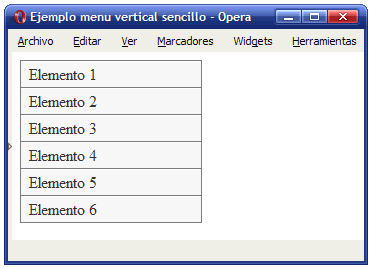
\includegraphics[width=0.6\textwidth]{figs/f0908.png}
\end{figure}
\end{center}

\end{frame}


%%---------------------------------------------------------------

\begin{frame}
\frametitle{Men� horizontal b�sico}

\begin{enumerate}
  \item Aplicar los estilos CSS b�sicos para establecer el estilo del men� (similares a los del men� vertical)
  \item  Establecer la anchura de los elementos del men�. Si el men� es de anchura variable y contiene cinco elementos, se asigna una anchura del 20\% a cada elemento
  \item Establecer los bordes de los elementos que forman el men�
  \item Se elimina el borde derecho del �ltimo elemento de la lista, para evitar el borde duplicado
\end{enumerate}


\begin{center}
\begin{figure}[p]
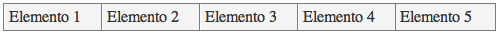
\includegraphics[width=0.8\textwidth]{figs/f0909.png}
\end{figure}
\end{center}

\end{frame}



%%---------------------------------------------------------------
%%---------------------------------------------------------------



\subsection*{CSS: Consideraciones adicionales}

\begin{frame}[fragile]
\frametitle{CSS: Consideraciones adicionales}

\begin{center}
{\Huge CSS \\ Consideraciones Adicionales}

{\footnotesize (transparencias de referencia)}

\end{center}


\end{frame}


%%---------------------------------------------------------------


\begin{frame}
\frametitle{Orden de visualizaci�n}

\begin{itemize}
  \item El relleno y el margen son transparentes, por lo que en el espacio ocupado por el relleno se muestra el color o imagen de fondo (si est�n definidos)
  \item En el espacio ocupado por el margen se muestra el color o imagen de fondo de su elemento padre (si est�n definidos)
  \item Si ning�n elemento padre tiene definido un color o imagen de fondo, se muestra el color o imagen de fondo de la propia p�gina (si est�n definidos)
  \item Si una caja define tanto un color como una imagen de fondo, la imagen tiene m�s prioridad y es la que se visualiza
  \item Si la imagen de fondo no cubre totalmente la caja del elemento o si la imagen tiene zonas transparentes, tambi�n se visualiza el color de fondo. 
\end{itemize}

\end{frame}



%%---------------------------------------------------------------

\begin{frame}
\frametitle{Propiedad width}

\begin{center}
  \begin{table}
   \begin{tabular}{p{1.8cm}p{7.8cm}}
Propiedad &\bf{width} \\ \hline
Valores & $<medida>$ | $<porcentaje>$ | auto | inherit \\ \hline
Se aplica a & Todos los elementos, salvo los elementos en l�nea que no sean im�genes, las filas de tabla y los grupos de filas de tabla \\ \hline
Valor inicial & auto \\ \hline
Descripci�n & Establece la anchura de un elemento \\ \hline
  \end{tabular}
   \caption{Definici�n de la propiedad \emph{width} de CSS}
 \end{table}
\end{center}

\end{frame}

%%---------------------------------------------------------------

\begin{frame}
\frametitle{Propiedad height}

\begin{center}
  \begin{table}
   \begin{tabular}{p{1.8cm}p{7.8cm}}
Propiedad &\bf{height} \\ \hline
Valores & $<medida>$ | $<porcentaje>$ | auto | inherit \\ \hline
Se aplica a & Todos los elementos, salvo los elementos en l�nea que no sean im�genes, las columnas de tabla y los grupos de columnas de tabla \\ \hline
Valor inicial & auto \\ \hline
Descripci�n & Establece la altura de un elemento \\ \hline
  \end{tabular}
   \caption{Definici�n de la propiedad \emph{height} de CSS}
 \end{table}
\end{center}

\end{frame}

%%---------------------------------------------------------------


\begin{frame}
\frametitle{M�rgenes}


\begin{center}
\begin{figure}[p]
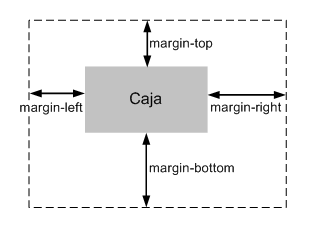
\includegraphics[width=0.45\textwidth]{figs/f0428.png}
\end{figure}
\end{center}

\begin{itemize}
  \item En vez de utilizar la etiqueta $<blockquote>$ de HTML, deber�a utilizarse la propiedad margin-left de CS
  \item Los m�rgenes verticales (margin-top y margin-bottom) s�lo se pueden aplicar a los elementos de bloque y las im�genes, mientras que los m�rgenes laterales (margin-left y margin-right) se pueden aplicar a cualquier elemento
\end{itemize}

\end{frame}


%%---------------------------------------------------------------

\begin{frame}
\frametitle{El margen vertical}

Es algo peculiar:

\begin{itemize}
  \item Cuando se juntan dos o m�s m�rgenes verticales, se fusionan de forma autom�tica y la altura del nuevo margen ser� igual a la altura del margen m�s alto de los que se han fusionado.
  \item Si un elemento est� contenido dentro de otro elemento, sus m�rgenes verticales se fusionan y resultan en un nuevo margen de la misma altura que el mayor margen de los que se han fusionado
  \item Si no se diera este comportamiento y se estableciera un determinado margen a todos los p�rrafos, el primer p�rrafo no mostrar�a un aspecto homog�neo respecto de los dem�s.
\end{itemize}

\end{frame}

%%---------------------------------------------------------------

\begin{frame}
\frametitle{Relleno}

\begin{center}
  \begin{table}
   \begin{tabular}{p{1.8cm}p{7.8cm}}
Propiedades &\bf{padding-top}, \bf{padding-right}, \bf{padding-bottom}, \bf{padding-left} \\ \hline
Valores & $<medida>$ | $<porcentaje>$ | inherit \\ \hline
Se aplica a & Todos los elementos excepto algunos elementos de tablas como grupos de cabeceras y grupos de pies de tabla \\ \hline
Valor inicial & 0 \\ \hline
Descripci�n & Establece cada uno de los rellenos horizontales y verticales de un elemento \\ \hline
  \end{tabular}
   \caption{Definici�n de la propiedad padding-top, padding-right, padding-bottom, padding-left de CSS}
 \end{table}
\end{center}

\end{frame}

%%---------------------------------------------------------------

\begin{frame}
\frametitle{}

\begin{center}
  \begin{table}
   \begin{tabular}{p{1.8cm}p{7.8cm}}
Propiedad &\bf{padding} \\ \hline
Valores & ( $<medida>$ | $<porcentaje>$ ) {1, 4} | inherit \\ \hline
Se aplica a & Todos los elementos excepto algunos elementos de tablas como grupos de cabeceras y grupos de pies de tabla \\ \hline
Valor inicial & - \\ \hline
Descripci�n & Establece de forma directa todos los rellenos de los elementos \\ \hline
  \end{tabular}
   \caption{Definici�n de la propiedad padding de CSS}
 \end{table}
\end{center}

\end{frame}

%%---------------------------------------------------------------

\begin{frame}
\frametitle{Anchura de los bordes}

\begin{center}
  \begin{table}
   \begin{tabular}{p{1.8cm}p{7.8cm}}
Propiedades &\bf{border-top-width}, \bf{border-right-width}, \bf{border-bottom-width}, \bf{border-left-width} \\ \hline
Valores & ( $<medida>$ | thin | medium | thick ) | inherit \\ \hline
Se aplica a & Todos los elementos \\ \hline
Valor inicial & Medium \\ \hline
Descripci�n & Establece la anchura de cada uno de los cuatro bordes de los elementos \\ \hline
  \end{tabular}
   \caption{Definici�n de la propiedad border-top-width, border-right-width, border-bottom-width, border-left-width de CSS}
 \end{table}
\end{center}

\end{frame}

%%---------------------------------------------------------------

\begin{frame}
\frametitle{Anchura de los bordes (shorthand)}

\begin{center}
  \begin{table}
   \begin{tabular}{p{1.8cm}p{7.8cm}}
Propiedad &\bf{border-width} \\ \hline
Valores & ( $<medida>$ | thin | medium | thick ) {1, 4} | inherit \\ \hline
Se aplica a & Todos los elementos \\ \hline
Valor inicial & Medium \\ \hline
Descripci�n & Establece la anchura de todos los bordes del elemento \\ \hline
  \end{tabular}
   \caption{Definici�n de la propiedad border-width de CSS}
 \end{table}
\end{center}

\end{frame}

%%---------------------------------------------------------------

\begin{frame}
\frametitle{Color de los bordes}

\begin{center}
  \begin{table}
   \begin{tabular}{p{1.8cm}p{7.8cm}}
Propiedades & \bf{border-top-color}, \bf{border-right-color}, \bf{border-bottom-color}, \bf{border-left-color} \\ \hline
Valores & $<color>$ | transparent | inherit \\ \hline
Se aplica a & Todos los elementos \\ \hline
Valor inicial & - \\ \hline
Descripci�n & Establece el color de cada uno de los cuatro bordes de los elementos \\ \hline
  \end{tabular}
   \caption{Definici�n de la propiedad border-top-color, border-right-color, border-bottom-color, border-left-color de CSS}
 \end{table}
\end{center}

\end{frame}

%%---------------------------------------------------------------

\begin{frame}
\frametitle{Color de los bordes (shorthand)}

\begin{center}
  \begin{table}
   \begin{tabular}{p{1.8cm}p{7.8cm}}
Propiedad &\bf{border-color} \\ \hline
Valores & ( $<color>$ | transparent ) {1, 4} | inherit \\ \hline
Se aplica a & Todos los elementos \\ \hline
Valor inicial & - \\ \hline
Descripci�n & Establece el color de todos los bordes del elemento \\ \hline
  \end{tabular}
   \caption{Definici�n de la propiedad border-color de CSS}
 \end{table}
\end{center}

\end{frame}

%%---------------------------------------------------------------

\begin{frame}
\frametitle{Estilo de los bordes}

\begin{center}
  \begin{table}
   \begin{tabular}{p{1.8cm}p{7.8cm}}
Propiedades &\bf{border-top-style}, \bf{border-right-style}, \bf{border-bottom-style}, \bf{border-left-style} \\ \hline
Valores & none | hidden | dotted | dashed | solid | double | groove | ridge | inset | outset | inherit \\ \hline
Se aplica a & Todos los elementos \\ \hline
Valor inicial & none \\ \hline
Descripci�n & Establece el estilo de cada uno de los cuatro bordes de los elementos \\ \hline
  \end{tabular}
   \caption{Definici�n de la propiedad border-top-style, border-right-style, border-bottom-style, border-left-style de CSS}
 \end{table}
\end{center}

\end{frame}

%%---------------------------------------------------------------

\begin{frame}
\frametitle{Estilo de los bordes \emph{shorthand}}

\begin{center}
  \begin{table}
   \begin{tabular}{p{1.8cm}p{7.8cm}}
Propiedad &\bf{border-style} \\ \hline
Valores & (none | hidden | dotted | dashed | solid | double | groove | ridge | inset | outset ) {1, 4} | inherit \\ \hline
Se aplica a & Todos los elementos \\ \hline
Valor inicial & - \\ \hline
Descripci�n & Establece el estilo de todos los bordes del elemento \\ \hline
  \end{tabular}
   \caption{Definici�n de la propiedad border-style de CSS}
 \end{table}
\end{center}

\end{frame}

%%---------------------------------------------------------------

\begin{frame}
\frametitle{Propiedades \emph{shorthand} para bordes}

\begin{center}
  \begin{table}
   \begin{tabular}{p{1.8cm}p{7.8cm}}
Propiedades &\bf{border-top}, \bf{border-right}, \bf{border-bottom}, \bf{border-left} \\ \hline
Valores & ( $<medida\_borde>$ || $<color\_borde>$ || $<estilo\_borde>$ ) | inherit \\ \hline
Se aplica a & Todos los elementos \\ \hline
Valor inicial & - \\ \hline
Descripci�n & Establece el estilo completo de cada uno de los cuatro bordes de los elementos \\ \hline
 \end{tabular}
   \caption{Definici�n de la propiedad border-top, border-right, border-bottom, border-left de CSS}
 \end{table}
\end{center}

\end{frame}

%%---------------------------------------------------------------

\begin{frame}
\frametitle{Propiedad \emph{shorthand} para borde (global)}

\begin{center}
  \begin{table}
   \begin{tabular}{p{1.8cm}p{7.8cm}}
Propiedad &\bf{border} \\ \hline
Valores & ( $<medida\_borde>$ || $<color\_borde>$ || $<estilo\_borde>$ ) | inherit \\ \hline
Se aplica a & Todos los elementos \\ \hline
Valor inicial & - \\ \hline
Descripci�n & Establece el estilo completo de todos los bordes de los elementos \\ \hline
 \end{tabular}
   \caption{Definici�n de la propiedad border de CSS}
 \end{table}
\end{center}

\end{frame}

%%---------------------------------------------------------------

\begin{frame}[fragile]
\frametitle{M�s sobre bordes}

\begin{itemize}
  \item Como el valor por defecto de la propiedad border-style es none, si una propiedad shorthand no establece expl�citamente el estilo de un borde, el elemento no muestra ese borde
  \item Cuando los cuatro bordes no son id�nticos pero s� muy parecidos, se puede utilizar la propiedad border para establecer de forma directa los atributos comunes de todos los bordes y posteriormente especificar para cada uno de los cuatro bordes sus propiedades particulares:
\begin{verbatim}
h1 {
  border: solid #000;
  border-top-width: 6px;
  border-left-width: 8px;
}
\end{verbatim}
\end{itemize}

\end{frame}

%%---------------------------------------------------------------

\begin{frame}
\frametitle{Fondos}

\begin{itemize}
  \item Puede ser un color simple o una imagen.
  \item Solamente se visualiza en el �rea ocupada por el contenido y su relleno, ya que el color de los bordes se controla directamente desde los bordes y las zonas de los m�rgenes siempre son transparentes
  \item Se puede establecer de forma simult�nea un color y una imagen de fondo. En este caso, la imagen se muestra delante del color, por lo que solamente si la imagen contiene zonas transparentes es posible ver el color de fondo.
\end{itemize}

\end{frame}


%%---------------------------------------------------------------

\begin{frame}
\frametitle{Propiedad background-color}

\begin{center}
  \begin{table}
   \begin{tabular}{p{1.8cm}p{7.8cm}}
Propiedad & \bf{background-color} \\ \hline
Valores& $color>$ | transparent | inherit \\ \hline
Se aplica a& Todos los elementos \\ \hline
Valor inicial& transparent \\ \hline
Descripci�n& Establece un color de fondo para los elementos \\ \hline
  \end{tabular}
   \caption{Definici�n de la propiedad background-color de CSS}
 \end{table}
\end{center}


\end{frame}


%%---------------------------------------------------------------

\begin{frame}
\frametitle{Propiedad background-image}

\begin{center}
  \begin{table}
   \begin{tabular}{p{1.8cm}p{7.8cm}}
Propiedad & \bf{background-image} \\ \hline
Valores& $url>$ | none | inherit \\ \hline
Se aplica a& Todos los elementos \\ \hline
Valor inicial& none \\ \hline
Descripci�n& Establece una imagen como fondo para los elementos \\ \hline
  \end{tabular}
   \caption{Definici�n de la propiedad background-image de CSS}
 \end{table}
\end{center}


\end{frame}


%%---------------------------------------------------------------

\begin{frame}
\frametitle{Propiedad background-repeat}

\begin{center}
  \begin{table}
   \begin{tabular}{p{1.8cm}p{7.8cm}}
Propiedad & \bf{background-repeat} \\ \hline
Valores& repeat | repeat-x | repeat-y | no-repeat | inherit \\ \hline
Se aplica a& Todos los elementos \\ \hline
Valor inicial& repeat \\ \hline
Descripci�n& Controla la forma en la que se repiten las im�genes de fondo \\ \hline
  \end{tabular}
   \caption{Definici�n de la propiedad background-repeat de CSS}
 \end{table}
\end{center}


\end{frame}


%%---------------------------------------------------------------

\begin{frame}
\frametitle{Propiedad background-position}

\begin{center}
  \begin{table}
   \begin{tabular}{p{1.8cm}p{7.8cm}}
Propiedad & \bf{background-position} \\ \hline
Valores& ( ( $<porcentaje>$ | $<medida>$ | left | center | right ) ( $<porcentaje>$ | $<medida>$ | top | center | bottom )? ) | ( ( left | center | right ) || ( top | center | bottom ) ) | inherit \\ \hline
Se aplica a& Todos los elementos \\ \hline
Valor inicial& 0\% 0\% \\ \hline
Descripci�n& Controla la posici�n en la que se muestra la imagen en el fondo del elemento \\ \hline
  \end{tabular}
   \caption{Definici�n de la propiedad background-position de CSS}
 \end{table}
\end{center}


\end{frame}


%%---------------------------------------------------------------

\begin{frame}
\frametitle{Propiedad background-attachment}

\begin{center}
  \begin{table}
   \begin{tabular}{p{1.8cm}p{7.8cm}}
Propiedad & \bf{background-attachment} \\ \hline
Valores& scroll | fixed | inherit \\ \hline
Se aplica a& Todos los elementos \\ \hline
Valor inicial& scroll \\ \hline
Descripci�n& Controla la forma en la que se visualiza la imagen de fondo: permanece fija cuando se hace scroll en la ventana del navegador o se desplaza junto con la ventana \\ \hline
  \end{tabular}
   \caption{Definici�n de la propiedad background-attachment de CSS}
 \end{table}
\end{center}


\end{frame}


%%---------------------------------------------------------------

\begin{frame}
\frametitle{Propiedad \emph{shorthand} background}

\begin{center}
  \begin{table}
   \begin{tabular}{p{1.8cm}p{7.8cm}}
Propiedad & \bf{background} \\ \hline
Valores& ( $background-color$ || $background-image$ || $background-repeat$ || $background-attachment$ || $background-position$ ) | inherit \\ \hline
Se aplica a& Todos los elementos \\ \hline
Valor inicial& - \\ \hline
Descripci�n& Establece todas las propiedades del fondo de un elemento \\ \hline
  \end{tabular}
   \caption{Definici�n de la propiedad background de CSS}
 \end{table}
\end{center}


\end{frame}



%%---------------------------------------------------------------
\subsubsection*{Posicionamiento y visualizaci�n}

%%---------------------------------------------------------------

\begin{frame}
\frametitle{Propiedad position}

\begin{center}
  \begin{table}
   \begin{tabular}{p{1.8cm}p{7.8cm}}
Propiedad & \bf{position} \\ \hline
Valores& static | relative | absolute | fixed | inherit \\ \hline
Se aplica a& Todos los elementos \\ \hline
Valor inicial& static \\ \hline
Descripci�n& Selecciona el posicionamiento con el que se mostrar� el elemento \\ \hline
  \end{tabular}
   \caption{Definici�n de la propiedad position de CSS}
 \end{table}
\end{center}


\end{frame}


%%---------------------------------------------------------------

\begin{frame}
\frametitle{Significados propiedad position}

\begin{itemize}
  \item static: corresponde al posicionamiento normal o est�tico. Si se utiliza este valor, se ignoran los valores de las propiedades top, right, bottom y left que se ver�n a continuaci�n.
  \item relative: corresponde al posicionamiento relativo. El desplazamiento de la caja se controla con las propiedades top, right, bottom y left.
  \item absolute: corresponde al posicionamiento absoluto. El desplazamiento de la caja tambi�n se controla con las propiedades top, right, bottom y left, pero su interpretaci�n es mucho m�s compleja, ya que el origen de coordenadas del desplazamiento depende del posicionamiento de su elemento contenedor.
  \item fixed: corresponde al posicionamiento fijo. El desplazamiento se establece de la misma forma que en el posicionamiento absoluto, pero en este caso el elemento permanece inamovible en la pantalla.
\end{itemize}

\end{frame}


%%---------------------------------------------------------------

\begin{frame}
\frametitle{Propiedades top, right, bottom, left}

\begin{center}
  \begin{table}
   \begin{tabular}{p{1.8cm}p{7.8cm}}
Propiedades& {\bf top}, {\bf right}, {\bf bottom}, {\bf left} \\ \hline
Valores& $<medida>$ | $<porcentaje>$ | auto | inherit \\ \hline
Se aplica a& Todos los elementos posicionados \\ \hline
Valor inicial& auto \\ \hline
Descripci�n& Indican el desplazamiento horizontal y vertical del elemento respecto de su posici�n original \\ \hline
  \end{tabular}
   \caption{Definici�n de la propiedad top, right, bottom, left de CSS}
 \end{table}
\end{center}


\end{frame}


%%---------------------------------------------------------------

\begin{frame}
\frametitle{Posicionamiento normal (o est�tico)}

\begin{itemize}
  \item Utilizado por defecto por los navegadores
  \item S�lo se tiene en cuenta si el elemento es de bloque o en l�nea, sus propiedades width y height y su contenido.
  \item Las cajas se muestran una debajo de otra comenzando desde el principio del elemento contenedor. La distancia entre las cajas se controla mediante los m�rgenes verticales.
  \item Si un elemento se encuentra dentro de otro, el elemento padre se llama ``elemento contenedor'' y determina tanto la posici�n como el tama�o de todas sus cajas interiores.
\end{itemize}


\begin{center}
\begin{figure}[p]
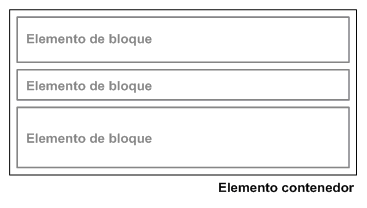
\includegraphics[width=0.8\textwidth]{figs/f0502.png}
\end{figure}
\end{center}

\end{frame}


%%---------------------------------------------------------------

\begin{frame}
\frametitle{Posicionamiento normal (o est�tico) (y II)}

\begin{itemize}
  \item Los elementos en l�nea forman los ``contextos de formato en l�nea''. Las cajas se muestran una detr�s de otra de forma horizontal comenzando desde la posici�n m�s a la izquierda de su elemento contenedor.
  \item Si las cajas en l�nea ocupan m�s espacio del disponible en su propia l�nea, el resto de cajas se muestran en las l�neas inferiores. 
  \item Si las cajas en l�nea ocupan un espacio menor que su propia l�nea, se puede controlar la distribuci�n de las cajas mediante la propiedad text-align para centrarlas, alinearlas a la derecha o justificarlas.
\end{itemize}


\begin{center}
\begin{figure}[p]
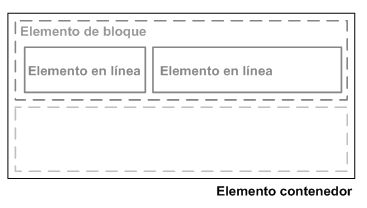
\includegraphics[width=0.8\textwidth]{figs/f0503.png}
\end{figure}
\end{center}

\end{frame}


%%---------------------------------------------------------------

\begin{frame}
\frametitle{Posicionamiento relativo}

\begin{itemize}
  \item Desplaza una caja respecto de su posici�n original establecida mediante el posicionamiento normal. El desplazamiento de la caja se controla con las propiedades top, right, bottom y left.
  \item la propiedad top se emplea para mover las cajas de forma descendente, la propiedad bottom mueve las cajas de forma ascendente, la propiedad left se utiliza para desplazar las cajas hacia la derecha y la propiedad right mueve las cajas hacia la izquierda. 
\end{itemize}

\begin{center}
\begin{figure}[p]
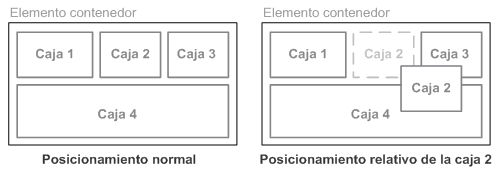
\includegraphics[width=0.8\textwidth]{figs/f0504.png}
\end{figure}
\end{center}

\end{frame}


%%---------------------------------------------------------------

\begin{frame}
\frametitle{Posicionamiento absoluto}

\begin{itemize}
  \item Se emplea para establecer de forma exacta la posici�n en la que se muestra la caja de un elemento. 
  \item Cuando una caja se posiciona de forma absoluta, el resto de elementos de la p�gina se ven afectados y modifican su posici�n. 
\end{itemize}

\begin{center}
\begin{figure}[p]
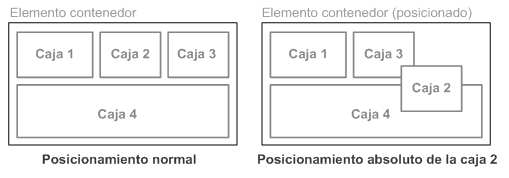
\includegraphics[width=0.8\textwidth]{figs/f0516.png}
\end{figure}
\end{center}

\end{frame}


%%---------------------------------------------------------------

\begin{frame}
\frametitle{Posicionamiento absoluto}

\begin{itemize}
  \item El primer elemento contenedor que est� posicionado de cualquier forma diferente a position: static se convierte en la referencia que determina la posici�n de la caja posicionada de forma absoluta.
  \item Si ning�n elemento contenedor est� posicionado, la referencia es la ventana del navegador, que no debe confundirse con el elemento $<body>$ de la p�gina.
  \item Una vez determinada la referencia del posicionamiento absoluto, la interpretaci�n de los valores de las propiedades top, right, bottom y left se realiza como sigue:
  \begin{itemize}
    \item Top: desplazamiento desde el borde superior del elemento contenedor que se utiliza como referencia.
    \item Right: �dem pero desde el borde derecho al borde derecho.
    \item Left:  �dem pero desde el borde izquierdo al borde izquierdo.
    \item Bottom: �dem pero desde el borde inferior al borde inferior.
  \end{itemize}
\end{itemize}

\end{frame}


%%---------------------------------------------------------------

\begin{frame}
\frametitle{Diferencias entre posicionamiento absoluto y relativo}

\begin{center}
\begin{figure}[p]
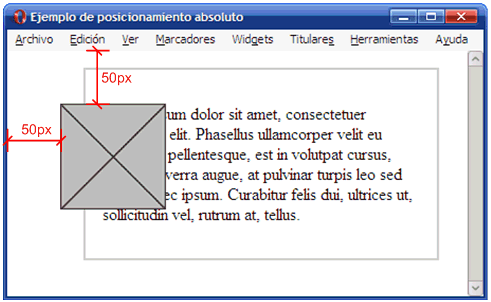
\includegraphics[width=0.6\textwidth]{figs/f0519.png}
\end{figure}
\end{center}

\begin{center}
\begin{figure}[p]
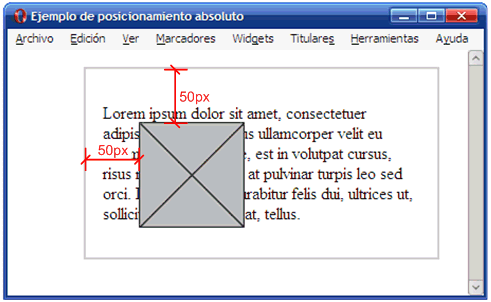
\includegraphics[width=0.6\textwidth]{figs/f0521.png}
\end{figure}
\end{center}

\end{frame}


%%---------------------------------------------------------------

\begin{frame}
\frametitle{Posicionamiento fijo}

\begin{itemize}
  \item Es un caso particular del posicionamiento absoluto, ya que s�lo se diferencian en el comportamiento de las cajas posicionadas.
  \item La principal caracter�stica de una caja posicionada de forma fija es que su posici�n es inamovible dentro de la ventana del navegador.
  \item El posicionamiento fijo hace que las cajas no modifiquen su posici�n ni aunque el usuario suba o baje la p�gina en la ventana de su navegador.
  \item Si la p�gina se visualiza en un medio paginado (por ejemplo en una impresora) las cajas posicionadas de forma fija se repiten en todas las p�ginas.
\end{itemize}

\end{frame}


%%---------------------------------------------------------------

\begin{frame}
\frametitle{Posicionamiento flotante}

\begin{itemize}
  \item Cuando una caja se posiciona con el modelo de posicionamiento flotante, autom�ticamente se convierte en una caja flotante, lo que significa que se desplaza hasta la zona m�s a la izquierda o m�s a la derecha de la posici�n en la que originalmente se encontraba.
\end{itemize}


\begin{center}
\begin{figure}[p]
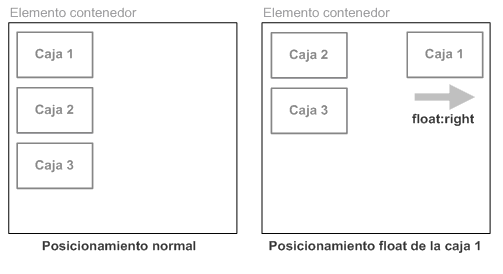
\includegraphics[width=0.8\textwidth]{figs/f0507.png}
\end{figure}
\end{center}

\end{frame}


%%---------------------------------------------------------------

\begin{frame}
\frametitle{Posicionamiento flotante (y II)}

\begin{itemize}
  \item Cuando se posiciona una caja de forma flotante:
  \begin{itemize}
    \item La caja deja de pertenecer al flujo normal de la p�gina, lo que significa que el resto de cajas ocupan el lugar dejado por la caja flotante.
    \item La caja flotante se posiciona lo m�s a la izquierda o lo m�s a la derecha posible de la posici�n en la que se encontraba originalmente.
  \end{itemize}
\end{itemize}


\begin{center}
\begin{figure}[p]
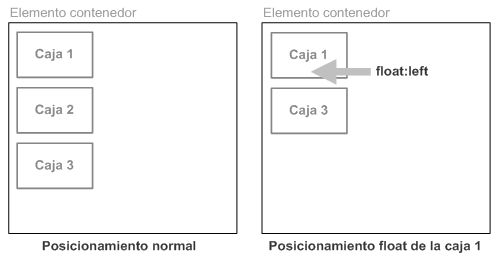
\includegraphics[width=0.8\textwidth]{figs/f0508.png}
\end{figure}
\end{center}

\end{frame}


%%---------------------------------------------------------------

\begin{frame}
\frametitle{Posicionamiento flotante (y III)}

\begin{itemize}
  \item Si existen otras cajas flotantes, al posicionar de forma flotante otra caja, se tiene en cuenta el sitio disponible.
  \item Si no existiera sitio en la l�nea actual, la caja flotante baja a la l�nea inferior hasta que encuentra el sitio necesario para mostrarse lo m�s a la izquierda o lo m�s a la derecha posible en esa nueva l�nea
\end{itemize}


\begin{center}
\begin{figure}[p]
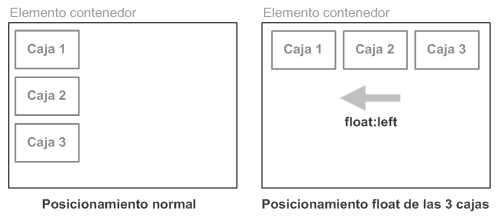
\includegraphics[width=0.8\textwidth]{figs/f0509.png}
\end{figure}
\end{center}

\end{frame}


%%---------------------------------------------------------------

\begin{frame}
\frametitle{Propiedad float}

\begin{center}
  \begin{table}
   \begin{tabular}{p{1.8cm}p{7.8cm}}
Propiedad & \bf{float} \\ \hline
Valores& left | right | none | inherit \\ \hline
Se aplica a& Todos los elementos \\ \hline
Valor inicial& none \\ \hline
Descripci�n& Establece el tipo de posicionamiento flotante del elemento \\ \hline
  \end{tabular}
   \caption{Definici�n de la propiedad float de CSS}
 \end{table}
\end{center}


\end{frame}


%%---------------------------------------------------------------

\begin{frame}
\frametitle{Posicionamiento flotante (y IV)}

\begin{itemize}
  \item Los elementos que se encuentran alrededor de una caja flotante adaptan sus contenidos para que fluyan alrededor del elemento posicionado
  \item Uno de los principales motivos para la creaci�n del posicionamiento float fue precisamente la posibilidad de colocar im�genes alrededor de las cuales fluye el texto.
\end{itemize}


\begin{center}
\begin{figure}[p]
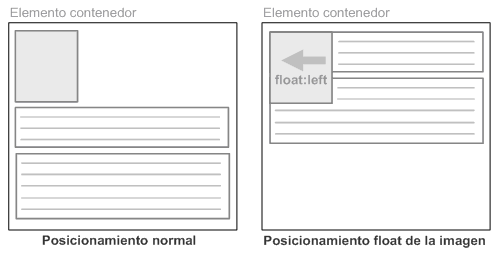
\includegraphics[width=0.8\textwidth]{figs/f0513.png}
\end{figure}
\end{center}

\end{frame}


%%---------------------------------------------------------------

\begin{frame}
\frametitle{Propiedad clear}

\begin{itemize}
  \item La propiedad clear indica el lado del elemento HTML que no debe ser adyacente a ninguna caja posicionada de forma flotante. Si se indica el valor left, el elemento se desplaza de forma descendente hasta que pueda colocarse en una l�nea en la que no haya ninguna caja flotante en el lado izquierdo.
  \item La especificaci�n oficial de CSS explica este comportamiento como ``un desplazamiento descendente hasta que el borde superior del elemento est� por debajo del borde inferior de cualquier elemento flotante hacia la izquierda''.
\end{itemize}

\end{frame}


%%---------------------------------------------------------------

\begin{frame}
\frametitle{Propiedad clear}

\begin{center}
  \begin{table}
   \begin{tabular}{p{1.8cm}p{7.8cm}}
Propiedad & \bf{clear} \\ \hline
Valores& none | left | right | both | inherit \\ \hline
Se aplica a& Todos los elementos de bloque \\ \hline
Valor inicial& none \\ \hline
Descripci�n& Indica el lado del elemento que no debe ser adyacente a ninguna caja flotante \\ \hline
  \end{tabular}
   \caption{Definici�n de la propiedad clear de CSS}
 \end{table}
\end{center}


\end{frame}



%%---------------------------------------------------------------

\begin{frame}
\frametitle{Propiedad display}

\begin{center}
  \begin{table}
   \begin{tabular}{p{1.8cm}p{7.8cm}}
Propiedad & \bf{display} \\ \hline
Valores& inline | block | none | list-item | run-in | inline-block | table | inline-table | table-row-group | table-header-group | table-footer-group | table-row | table-column-group | table-column | table-cell | table-caption | inherit \\ \hline
Se aplica a& Todos los elementos \\ \hline
Valor inicial& inline \\ \hline
Descripci�n& Permite controlar la forma de visualizar un elemento e incluso ocultarlo \\ \hline
  \end{tabular}
   \caption{Definici�n de la propiedad display de CSS}
 \end{table}
\end{center}


\end{frame}




%%---------------------------------------------------------------

\begin{frame}
\frametitle{Propiedad visibility}

\begin{center}
  \begin{table}
   \begin{tabular}{p{1.8cm}p{7.8cm}}
Propiedad & \bf{visibility} \\ \hline
Valores& visible | hidden | collapse | inherit \\ \hline
Se aplica a& Todos los elementos \\ \hline
Valor inicial& visible \\ \hline
Descripci�n& Permite hacer visibles e invisibles a los elementos \\ \hline
  \end{tabular}
   \caption{Definici�n de la propiedad visibility de CSS}
 \end{table}
\end{center}


\end{frame}


%%---------------------------------------------------------------

\begin{frame}
\frametitle{Propiedad overflow}

\begin{itemize}
  \item En algunas ocasiones el contenido de un elemento no cabe en el espacio reservado para ese elemento y se desborda.
  \item La situaci�n m�s habitual en la que el contenido sobresale de su espacio reservado es cuando se establece la anchura y/o altura de un elemento mediante la propiedad width y/o height. 
  \item Los valores de la propiedad overflow tienen el siguiente significado:
  \begin{itemize}
    \item visible: el contenido no se corta y se muestra sobresaliendo la zona reservada para visualizar el elemento. Este es el comportamiento por defecto.
    \item hidden: el contenido sobrante se oculta y s�lo se visualiza la parte del contenido que cabe dentro de la zona reservada para el elemento.
    \item scroll: solamente se visualiza el contenido que cabe dentro de la zona reservada para el elemento, pero tambi�n se muestran barras de scroll que permiten visualizar el resto del contenido.
    \item auto: el comportamiento depende del navegador, aunque normalmente es el mismo que la propiedad scroll.
  \end{itemize}
\end{itemize}

\end{frame}


%%---------------------------------------------------------------

\begin{frame}
\frametitle{Propiedad overflow (y II)}

\begin{center}
\begin{figure}[p]
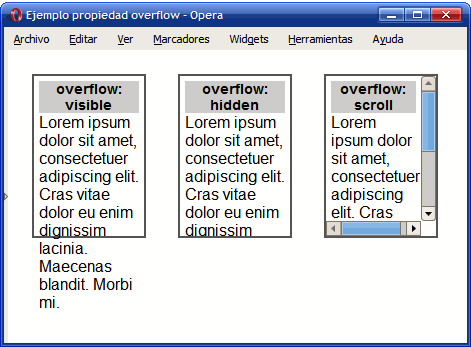
\includegraphics[width=0.8\textwidth]{figs/f0524.png}
\end{figure}
\end{center}

\end{frame}


%%---------------------------------------------------------------

\begin{frame}
\frametitle{Propiedad overflow (y III)}

\begin{center}
  \begin{table}
   \begin{tabular}{p{1.8cm}p{7.8cm}}
Propiedad & \bf{overflow} \\ \hline
Valores& visible | hidden | scroll | auto | inherit \\ \hline
Se aplica a& Elementos de bloque y celdas de tablas \\ \hline
Valor inicial& visible \\ \hline
Descripci�n& Permite controlar los contenidos sobrantes de un elemento \\ \hline
  \end{tabular}
   \caption{Definici�n de la propiedad overflow de CSS}
 \end{table}
\end{center}


\end{frame}



%%---------------------------------------------------------------

\begin{frame}
\frametitle{Propiedad z-index}

\begin{itemize}
  \item CSS permite controlar la posici�n tridimensional de las cajas posicionadas
  \item Es posible indicar las cajas que se muestran delante o detr�s de otras cajas cuando se producen solapamientos.
  \item Cuanto m�s alto sea el valor num�rico, m�s cerca del usuario se muestra la caja.
\end{itemize}

\end{frame}


%%---------------------------------------------------------------

\begin{frame}
\frametitle{Propiedad z-index (II)}


\begin{center}
\begin{figure}[p]
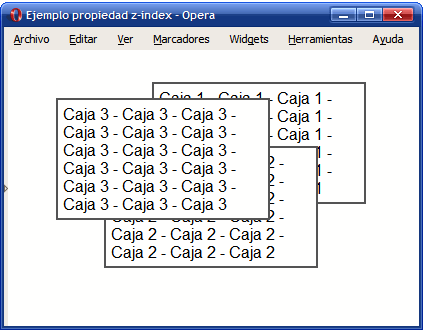
\includegraphics[width=0.66\textwidth]{figs/f0525.png}
\end{figure}
\end{center}

\end{frame}



%%---------------------------------------------------------------

\begin{frame}
\frametitle{Propiedad z-index (y III)}

\begin{center}
  \begin{table}
   \begin{tabular}{p{1.8cm}p{7.8cm}}
Propiedad & \bf{z-index} \\ \hline
Valores& auto | $<numero>$ | inherit \\ \hline
Se aplica a& Elementos que han sido posicionados expl�citamente \\ \hline
Valor inicial& auto \\ \hline
Descripci�n& Establece el nivel tridimensional en el que se muestra el elemento \\ \hline
  \end{tabular}
   \caption{Definici�n de la propiedad z-index de CSS}
 \end{table}
\end{center}


\end{frame}

%%---------------------------------------------------------------

\begin{frame}[fragile]
\frametitle{Selectores avanzados}

\begin{enumerate}
  \item Selector de hijos
\begin{verbatim}
p > span { color: blue; }
\end{verbatim}
  \item Selector adyacente
\begin{verbatim}
p + p { text-indent: 1.5em; }
\end{verbatim}
  \item Selector de atributos
\begin{verbatim}
a[class="externo"] { color: blue; }
a[class~="externo"] { color: blue; }
*[lang=en] { ... }
*[lang|="es"] { color : red }
\end{verbatim}
\end{enumerate}

\end{frame}



%%---------------------------------------------------------------

\begin{frame}
\frametitle{Colisi�n de estilos}

El m�todo seguido por CSS para resolver las colisiones de estilos se muestra a continuaci�n:

\begin{enumerate}
  \item Determinar todas las declaraciones que se aplican al elemento para el medio CSS seleccionado.
  \item Ordenar las declaraciones seg�n su origen (CSS de navegador, de usuario o de dise�ador) y su prioridad (palabra clave !important).
  \item Ordenar las declaraciones seg�n lo espec�fico que sea el selector. Cuanto m�s gen�rico es un selector, menos importancia tienen sus declaraciones.
  \item Si despu�s de aplicar las normas anteriores existen dos o m�s reglas con la misma prioridad, se aplica la que se indic� en �ltimo lugar.
\end{enumerate}

\end{frame}



%%---------------------------------------------------------------

\begin{frame}
\frametitle{Medios CSS}

\begin{itemize}
  \item Permiten definir diferentes estilos para diferentes medios o dispositivos: pantallas, impresoras, m�viles, proyectores, etc.
  \item Define algunas propiedades espec�ficamente para determinados medios: la paginaci�n y los saltos de p�gina para los medios impresos o el volumen y tipo de voz para los medios de audio.
  \item Ejemplos:
  \begin{itemize}
    \item screen: Pantallas de ordenador
    \item print: Impresoras y navegadores en el modo ``Vista Previa para Imprimir''
    \item handheld:	Dispositivos de mano: m�viles, PDA, etc.
  \end{itemize}
\end{itemize}

\end{frame}

%%---------------------------------------------------------------

\begin{frame}[fragile]
\frametitle{Formas de indicar el medio}

\begin{enumerate}
  \item Reglas de tipo @media
{\footnotesize
    \begin{verbatim}
@media print {
  body { font-size: 10pt }
}
@media screen {
  body { font-size: 13px }
}
    \end{verbatim}
}
  \item Reglas de tipo @import
{\footnotesize
    \begin{verbatim}
@import url("estilos_basicos.css") screen;
@import url("estilos_impresora.css") print;
    \end{verbatim}
}
  \item Medios definidos con la etiqueta
{\footnotesize
    \begin{verbatim}
<link rel="stylesheet" type="text/css" media="screen" href="basico.css" />
<link rel="stylesheet" type="text/css" media="print, handheld" href="especial.css" />
    \end{verbatim}
}
  \item Medios definidos mezclando varios m�todos
{\footnotesize
    \begin{verbatim}
<link rel="stylesheet" type="text/css"  media="screen" href="basico.css" />
@import url("estilos_seccion.css") screen;
@media print {
  /* Estilos espec�ficos para impresora */
}
    \end{verbatim}
}
\end{enumerate}

\end{frame}

%%---------------------------------------------------------------

\begin{frame}[fragile]
\frametitle{Comentarios}

\begin{itemize}
  \item El comienzo de un comentario se indica mediante los caracteres /* y el final del comentario se indica mediante */
    \begin{verbatim}
/* Este es un comentario en CSS */
    \end{verbatim}
  \item Pueden ocupar tantas l�neas como sea necesario, pero no se puede incluir un comentario dentro de otro comentario
    \begin{verbatim}
/* Este es un
   comentario CSS de varias
   lineas */
    \end{verbatim}
\end{itemize}

\end{frame}


%%---------------------------------------------------------------
\subsubsection*{Texto}

\begin{frame}
\frametitle{Tipograf�a}

\begin{itemize}
  \item CSS define numerosas propiedades para modificar la apariencia del texto
  \item color se utiliza para establecer el color de la letra
  \item Como el valor de la propiedad color se hereda, normalmente se establece la propiedad color en el elemento body para establecer el color de letra de todos los elementos de la p�gina
 \item font-family se utiliza para indicar el tipo de letra con el que se muestra el texto
  \item Suele definirse como una lista de tipos de letra alternativos separados por comas. El �ltimo valor de la lista es el nombre de la familia tipogr�fica gen�rica que m�s se parece al tipo de letra que se quiere utilizar.
\end{itemize}

\end{frame}


%%---------------------------------------------------------------

\begin{frame}
\frametitle{Propiedad color}

\begin{center}
  \begin{table}
   \begin{tabular}{p{1.8cm}p{7.8cm}}
Propiedad & \bf{color} \\ \hline
Valores& $<color>$ | inherit \\ \hline
Se aplica a& Todos los elementos \\ \hline
Valor inicial& Depende del navegador \\ \hline
Descripci�n& Establece el color de letra utilizado para el texto \\ \hline
  \end{tabular}
   \caption{Definici�n de la propiedad color de CSS}
 \end{table}
\end{center}


\end{frame}


%%---------------------------------------------------------------

\begin{frame}
\frametitle{Propiedad font-family}

\begin{center}
  \begin{table}
   \begin{tabular}{p{1.8cm}p{7.8cm}}
Propiedad & \bf{font-family} \\ \hline
Valores& (( $<nombre\_familia>$ | $<familia\_generica>$ ) (,$nombre\_familia>$ | $<familia\_generica$)* ) | inherit \\ \hline
Se aplica a& Todos los elementos \\ \hline
Valor inicial& Depende del navegador \\ \hline
Descripci�n& Establece el tipo de letra utilizado para el texto \\ \hline
  \end{tabular}
   \caption{Definici�n de la propiedad font-family de CSS}
 \end{table}
\end{center}


\end{frame}


%%---------------------------------------------------------------

\begin{frame}
\frametitle{Propiedad font-size (I)}

\begin{itemize}
  \item Adem�s de medida relativas, absolutas y de porcentajes, CSS permite utilizar una serie de palabras clave para indicar el tama�o de letra del texto:
  \begin{itemize}
    \item tama�o\_absoluto: indica el tama�o de letra de forma absoluta mediante alguna de las siguientes palabras clave: xx-small, x-small, small, medium, large, x-large, xx-large.
    \item tama�o\_relativo: indica de forma relativa el tama�o de letra del texto mediante dos palabras clave (larger, smaller) que toman como referencia el tama�o de letra del elemento padre.
  \end{itemize}
\end{itemize}


\begin{center}
\begin{figure}[p]
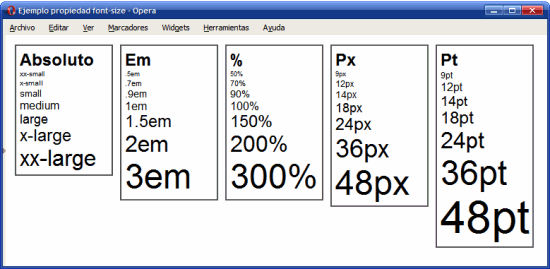
\includegraphics[width=0.6\textwidth]{figs/f0601.png}
\end{figure}
\end{center}

\end{frame}


%%---------------------------------------------------------------

\begin{frame}
\frametitle{Propiedad font-size (y II)}

\begin{center}
  \begin{table}
   \begin{tabular}{p{1.8cm}p{7.8cm}}
Propiedad & \bf{font-size} \\ \hline
Valores & $<tamano\_absoluto>$ | $<tamano\_relativo>$ | $<medida>$ | $<porcentaje>$ | inherit \\ \hline
Se aplica a & Todos los elementos \\ \hline
Valor inicial & medium \\ \hline
Descripci�n & Establece el tama�o de letra utilizado para el texto \\ \hline
  \end{tabular}
   \caption{Definici�n de la propiedad font-size de CSS}
 \end{table}
\end{center}

\end{frame}


%%---------------------------------------------------------------

\begin{frame}
\frametitle{Propiedad font-weight}

\begin{center}
  \begin{table}
   \begin{tabular}{p{1.8cm}p{7.8cm}}
Propiedad & \bf{font-weight} \\ \hline
Valores& normal | bold | bolder | lighter | 100 | 200 | 300 | 400 | 500 | 600 | 700 | 800 | 900 | inherit \\ \hline
Se aplica a& Todos los elementos \\ \hline
Valor inicial& normal \\ \hline
Descripci�n& Establece la anchura de la letra utilizada para el texto \\ \hline
  \end{tabular}
   \caption{Definici�n de la propiedad font-weight de CSS}
 \end{table}
\end{center}


\end{frame}


%%---------------------------------------------------------------

\begin{frame}
\frametitle{Propiedad font-style}

\begin{center}
  \begin{table}
   \begin{tabular}{p{1.8cm}p{7.8cm}}
Propiedad & \bf{font-style} \\ \hline
Valores& normal | italic | oblique | inherit \\ \hline
Se aplica a& Todos los elementos \\ \hline
Valor inicial& normal \\ \hline
Descripci�n& Establece el estilo de la letra utilizada para el texto \\ \hline
  \end{tabular}
   \caption{Definici�n de la propiedad font-style de CSS}
 \end{table}
\end{center}

\end{frame}


%%---------------------------------------------------------------

\begin{frame}
\frametitle{Propiedad font-variant}

\begin{center}
  \begin{table}
   \begin{tabular}{p{1.8cm}p{7.8cm}}
Propiedad & \bf{font-variant} \\ \hline
Valores& normal | small-caps | inherit \\ \hline
Se aplica a& Todos los elementos \\ \hline
Valor inicial& normal \\ \hline
Descripci�n& Establece el estilo alternativo de la letra utilizada para el texto \\ \hline
  \end{tabular}
   \caption{Definici�n de la propiedad font-variant de CSS}
 \end{table}
\end{center}


\end{frame}


%%---------------------------------------------------------------

\begin{frame}
\frametitle{Propiedad \emph{short-hand} font}

\begin{center}
  \begin{table}
   \begin{tabular}{p{1.8cm}p{7.8cm}}
Propiedad & \bf{font} \\ \hline
Valores& ( ( $<font-style>$ || $<font-variant>$ || $<font-weight>$ )? $<font-size>$ ( / $<line-height>$ )? $<font-family>$ ) | caption | icon | menu | message-box | small-caption | status-bar | inherit \\ \hline
Se aplica a& Todos los elementos \\ \hline
Valor inicial& - \\ \hline
Descripci�n& Permite indicar de forma directa todas las propiedades de la tipograf�a de un texto \\ \hline
  \end{tabular}
   \caption{Definici�n de la propiedad font de CSS}
 \end{table}
\end{center}


\end{frame}


%%---------------------------------------------------------------

\begin{frame}[fragile]
\frametitle{Propiedad \emph{short-hand} font (y II)}

\begin{itemize}
  \item El orden en el que se deben indicar las propiedades del texto es el siguiente:
  \begin{itemize}
    \item En primer lugar y de forma opcional se indican el font-style, font-variant y font-weight en cualquier orden.
    \item A continuaci�n, se indica obligatoriamente el valor de font-size seguido opcionalmente por el valor de line-height.
    \item Por �ltimo, se indica obligatoriamente el tipo de letra a utilizar.
  \end{itemize}
\end{itemize}

\begin{footnotesize}
\begin{verbatim}
font: bold 1em "Trebuchet MS",Arial,Sans-Serif;
font: normal 0.9em "Lucida Grande", Verdana, Arial, Helvetica, sans-serif;
font: normal 1.2em/1em helvetica, arial, sans-serif;
\end{verbatim}
\end{footnotesize}

\end{frame}


%%---------------------------------------------------------------

\begin{frame}
\frametitle{Texto}

\begin{itemize}
  \item Adem�s de las propiedades relativas a la tipograf�a del texto, CSS define numerosas propiedades que determinan la apariencia del texto en su conjunto.
  \item Estas propiedades adicionales permiten controlar
  \begin{itemize}
    \item la alineaci�n del texto,
    \item el interlineado,
    \item la separaci�n entre palabras,
    \item etc.
  \end{itemize}
\end{itemize}

\end{frame}


%%---------------------------------------------------------------

\begin{frame}
\frametitle{Propiedad text-align}

\begin{center}
  \begin{table}
   \begin{tabular}{p{1.8cm}p{7.8cm}}
Propiedad & \bf{text-align} \\ \hline
Valores& left | right | center | justify | inherit \\ \hline
Se aplica a& Elementos de bloque y celdas de tabla \\ \hline
Valor inicial& left \\ \hline
Descripci�n& Establece la alineaci�n del contenido del elemento \\ \hline
  \end{tabular}
   \caption{Definici�n de la propiedad text-align de CSS}
 \end{table}
\end{center}


\end{frame}


%%---------------------------------------------------------------

\begin{frame}
\frametitle{Propiedad line-height}

\begin{center}
  \begin{table}
   \begin{tabular}{p{1.8cm}p{7.8cm}}
Propiedad & \bf{line-height} \\ \hline
Valores& normal | $<numero>$ | $<medida>$ | $<porcentaje>$ | inherit \\ \hline
Se aplica a& Todos los elementos \\ \hline
Valor inicial& normal \\ \hline
Descripci�n& Permite establecer la altura de l�nea de los elementos \\ \hline
  \end{tabular}
   \caption{Definici�n de la propiedad line-height de CSS}
 \end{table}
\end{center}


\end{frame}


%%---------------------------------------------------------------

\begin{frame}
\frametitle{Propiedad text-decoration}

\begin{center}
  \begin{table}
   \begin{tabular}{p{1.8cm}p{7.8cm}}
Propiedad & \bf{text-decoration} \\ \hline
Valores& none | ( underline || overline || line-through || blink ) | inherit \\ \hline
Se aplica a& Todos los elementos \\ \hline
Valor inicial& none \\ \hline
Descripci�n& Establece la decoraci�n del texto (subrayado, tachado, parpadeante, etc.) \\ \hline
  \end{tabular}
   \caption{Definici�n de la propiedad text-decoration de CSS}
 \end{table}
\end{center}


\end{frame}


%%---------------------------------------------------------------

\begin{frame}
\frametitle{Propiedad text-transform}

\begin{center}
  \begin{table}
   \begin{tabular}{p{1.8cm}p{7.8cm}}
Propiedad & \bf{text-transform} \\ \hline
Valores& capitalize | uppercase | lowercase | none | inherit \\ \hline
Se aplica a& Todos los elementos \\ \hline
Valor inicial& none \\ \hline
Descripci�n& Transforma el texto original (lo transforma a may�sculas, a min�sculas, etc.) \\ \hline
  \end{tabular}
   \caption{Definici�n de la propiedad text-transform de CSS}
 \end{table}
\end{center}


\end{frame}


%%---------------------------------------------------------------

\begin{frame}
\frametitle{Propiedad vertical-align}

\begin{center}
  \begin{table}
   \begin{tabular}{p{1.8cm}p{7.8cm}}
Propiedad & \bf{vertical-align} \\ \hline
Valores& baseline | sub | super | top | text-top | middle | bottom | text-bottom | $<porcentaje>$ | $<medida>$ | inherit \\ \hline
Se aplica a& Elementos en l�nea y celdas de tabla \\ \hline
Valor inicial& baseline \\ \hline
Descripci�n& Determina la alineaci�n vertical de los contenidos de un elemento \\ \hline
  \end{tabular}
   \caption{Definici�n de la propiedad vertical-align de CSS}
 \end{table}
\end{center}


\end{frame}


%%---------------------------------------------------------------

\begin{frame}
\frametitle{Propiedad text-indent}

\begin{center}
  \begin{table}
   \begin{tabular}{p{1.8cm}p{7.8cm}}
Propiedad & \bf{text-indent} \\ \hline
Valores& $<medida>$ | $<porcentaje>$ | inherit \\ \hline
Se aplica a& Los elementos de bloque y las celdas de tabla \\ \hline
Valor inicial& 0 \\ \hline
Descripci�n& Tabula desde la izquierda la primera l�nea del texto original \\ \hline
  \end{tabular}
   \caption{Definici�n de la propiedad text-indent de CSS}
 \end{table}
\end{center}


\end{frame}


%%---------------------------------------------------------------

\begin{frame}
\frametitle{Propiedad letter-spacing}

\begin{center}
  \begin{table}
   \begin{tabular}{p{1.8cm}p{7.8cm}}
Propiedad & \bf{letter-spacing} \\ \hline
Valores& normal | $<medida>$ | inherit \\ \hline
Se aplica a& Todos los elementos \\ \hline
Valor inicial& normal \\ \hline
Descripci�n& Permite establecer el espacio entre las letras que forman las palabras del texto \\ \hline
  \end{tabular}
   \caption{Definici�n de la propiedad letter-spacing de CSS}
 \end{table}
\end{center}


\end{frame}


%%---------------------------------------------------------------

\begin{frame}
\frametitle{Propiedad word-spacing}

\begin{center}
  \begin{table}
   \begin{tabular}{p{1.8cm}p{7.8cm}}
Propiedad & \bf{word-spacing} \\ \hline
Valores& normal | $<medida>$ | inherit \\ \hline
Se aplica a& Todos los elementos \\ \hline
Valor inicial& normal \\ \hline
Descripci�n& Permite establecer el espacio entre las palabras que forman el texto \\ \hline
  \end{tabular}
   \caption{Definici�n de la propiedad word-spacing de CSS}
 \end{table}
\end{center}


\end{frame}


%%---------------------------------------------------------------

\begin{frame}
\frametitle{Propiedad white-space}

\begin{center}
  \begin{table}
   \begin{tabular}{p{1.8cm}p{7.8cm}}
Propiedad & \bf{white-space} \\ \hline
Valores& normal | pre | nowrap | pre-wrap | pre-line | inherit \\ \hline
Se aplica a& Todos los elementos \\ \hline
Valor inicial& normal \\ \hline
Descripci�n& Establece el tratamiento de los espacios en blanco del texto \\ \hline
  \end{tabular}
   \caption{Definici�n de la propiedad white-space de CSS}
 \end{table}
\end{center}


\end{frame}


%%---------------------------------------------------------------

\begin{frame}
\frametitle{Propiedad white-space (y II)}

El significado de cada uno de los valores es el siguiente:
\begin{itemize}
  \item normal: comportamiento por defecto de HTML.
  \item pre: se respetan los espacios en blanco y las nuevas l�neas (exactamente igual que la etiqueta $<pre>$). Si la l�nea es muy larga, se sale del espacio asignado para ese contenido.
  \item nowrap: elimina los espacios en blanco y las nuevas l�neas. Si la l�nea es muy larga, se sale del espacio asignado para ese contenido.
  \item pre-wrap: se respetan los espacios en blanco y las nuevas l�neas, pero ajustando cada l�nea al espacio asignado para ese contenido.
  \item pre-line: elimina los espacios en blanco y respeta las nuevas l�neas, pero ajustando cada l�nea al espacio asignado para ese contenido.
\end{itemize}

\end{frame}



%%---------------------------------------------------------------

\subsubsection*{Listas}

\begin{frame}
\frametitle{Propiedad list-style-type}

\begin{center}
  \begin{table}
   \begin{tabular}{p{1.8cm}p{7.8cm}}
Propiedad & \bf{list-style-type} \\ \hline
Valores& disc | circle | square | decimal | decimal-leading-zero | lower-roman | upper-roman | lower-greek | lower-latin | upper-latin | armenian | georgian | lower-alpha | upper-alpha | none | inherit \\ \hline
Se aplica a& Elementos de una lista \\ \hline
Valor inicial& disc \\ \hline
Descripci�n& Permite establecer el tipo de vi�eta mostrada para una lista \\ \hline
  \end{tabular}
   \caption{Definici�n de la propiedad list-style-type de CSS}
 \end{table}
\end{center}


\end{frame}


%%---------------------------------------------------------------

\begin{frame}
\frametitle{Propiedad list-style-position}

\begin{center}
  \begin{table}
   \begin{tabular}{p{1.8cm}p{7.8cm}}
Propiedad & \bf{list-style-position} \\ \hline
Valores& inside | outside | inherit \\ \hline
Se aplica a& Elementos de una lista \\ \hline
Valor inicial& outside \\ \hline
Descripci�n& Permite establecer la posici�n de la vi�eta de cada elemento de una lista \\ \hline
  \end{tabular}
   \caption{Definici�n de la propiedad list-style-type de CSS}
 \end{table}
\end{center}


\end{frame}


%%---------------------------------------------------------------

\begin{frame}
\frametitle{Propiedad list-style-image}

\begin{center}
  \begin{table}
   \begin{tabular}{p{1.8cm}p{7.8cm}}
Propiedad & \bf{list-style-image} \\ \hline
Valores& $<url>$ | none | inherit \\ \hline
Se aplica a& Elementos de una lista \\ \hline
Valor inicial& none \\ \hline
Descripci�n& Permite reemplazar las vi�etas autom�ticas por una imagen personalizada \\ \hline
  \end{tabular}
   \caption{Definici�n de la propiedad list-style-image de CSS}
 \end{table}
\end{center}


\end{frame}


%%---------------------------------------------------------------

\begin{frame}
\frametitle{Propiedad \emph{shorthand} list-style}

\begin{center}
  \begin{table}
   \begin{tabular}{p{1.8cm}p{7.8cm}}
Propiedad & \bf{list-style} \\ \hline
Valores& ( $<list-style-type>$ || $<list-style-position>$ || $<list-style-image>$ ) | inherit \\ \hline
Se aplica a& Elementos de una lista \\ \hline
Valor inicial& - \\ \hline
Descripci�n& Propiedad que permite establecer de forma simult�nea todas las opciones de una lista \\ \hline
  \end{tabular}
   \caption{Definici�n de la propiedad list-style de CSS}
 \end{table}
\end{center}


\end{frame}




%%---------------------------------------------------------------

%\begin{frame}
%\frametitle{}

%\begin{itemize}
%  \item 
%\end{itemize}
%
%\end{frame}




% $Id: $
%
%

\section{Pr�cticas: Introducci�n a Python}

%-----------------------    ---------------------------------
\usebackgroundtemplate{
\includegraphics[width=13cm]{figs/yoda.jpg}}

\begin{frame}
\frametitle{Python}

\end{frame}
\usebackgroundtemplate{}


\subsection{Transparencias principales}

\begin{frame}
\frametitle{Transparencias principales}

\begin{center}
{\Huge Transparencias principales}

{\footnotesize (las que veremos en clase)}
\end{center}
\end{frame}


\begin{frame}[fragile]

\frametitle{Hola Mundo}

\begin{itemize}
\item Desde la shell, accede al int�rprete de Python 3:

\begin{footnotesize}
\begin{verbatim}
$ python3
>>>
\end{verbatim}
\end{footnotesize}
\item Y ya podemos introducir instrucciones en Python:

\begin{footnotesize}
\begin{verbatim}
>>> print("hola mundo")
hola mundo
\end{verbatim}
\end{footnotesize}

\item A partir de ahora obviaremos generalmente los $>>>$ del int�rprete.

\end{itemize}

\end{frame}



\begin{frame}[fragile]

\frametitle{M�s ejemplos}

\begin{itemize}
\item Podemos usar Python como calculadora\\
(ojo: 3/2=1)

\item Ver�s que Python es sensible may�sculas

\item En Python hay diferentes tipos de datos

\item Los comentarios se indican con \verb=#=

\end{itemize}

\begin{footnotesize}
\begin{verbatim}
print("hola mundo")    # esto es un comentario
euro = 415
pesetas = euro * 166.386
print(str(euro) + " euro are "+ str(pesetas) + " pesetas")
\end{verbatim}
\end{footnotesize}

\end{frame}



\begin{frame}[fragile]
\frametitle{Sangrado y separadores de sentencias}

\begin{itemize}
\item �En Python NO hay llaves ni \verb|begin-end| para encerrar bloques
  de c�digo!
\item Un mayor nivel de sangrado indica que comienza un bloque,
  y un menor nivel indica que termina un bloque.
  
\item Ejemplo:

  \begin{footnotesize}
\begin{verbatim}
# Two Python functions
def to_celsius(faren):
    """Converts farenheit into celsius"""
    return (faren - 32) * (5.0/9)


def to_farenheit(cels):
    """Converts celsius into farenheit"""
    return (cels * 1.8) + 32
\end{verbatim}
  \end{footnotesize}
\end{itemize}
\end{frame}




\begin{frame}[fragile]
\frametitle{Condicional}

Sentencia \verb|if|:

\begin{footnotesize}
\begin{verbatim}
integer = 3
if integer:
     print('True')
else:
     print('False')
\end{verbatim}
\end{footnotesize}
N�tese como el caracter \verb|:| introduce cada bloque de sentencias. Si hay \verb|:|, entonces la siguiente l�nea estar� indentada.
%se pueden poner parentesis en la condici�n, como en C, pero no necesario
\end{frame}



\begin{frame}[fragile]
\frametitle{Cadenas}

\begin{itemize}
\item No existe tipo \verb|char|
\item 
Comilla simple o doble \\
\verb|print("hola")|  o \verb|print('hola')|  \\
\verb|print 'me dijo "hola"'| \\
m�s legible que \verb|print('me dijo \'hola\'')|
\item 
Puede haber caracteres especiales\\
\verb|print("hola\nque tal")|   

\item El operador \verb|+| concatena cadenas, y el \verb|*| las repite
  un n�mero entero de veces
\end{itemize}
\end{frame}


\begin{frame}[fragile]
\frametitle{Listas}

\begin{itemize}
\item Tipo de datos predefinido en Python, va mucho m�s all� de los
  arrays
\item Es un conjunto {\bf indexado} de elementos, no necesariamente homog�neos
\item Sintaxis:Identificador de lista, mas �ndice entre corchetes
\item Cada elemento se separa del anterior por un caracter \verb|,|
\end{itemize}
  \begin{footnotesize}
\begin{verbatim}
colors = ['red', 'yellow']
colors.append('green')
print(colors)
print(colors[2])
print(len(colors))

things = ['string', 2, 3.0]

\end{verbatim}
  \end{footnotesize}

\end{frame}



\begin{frame}[fragile]
\frametitle{M�s sobre listas}

\begin{itemize}
\item El primer elemento tiene �ndice 0.
\item Un �ndice negativo accede a los elementos empezando por el final
  de la lista. El �ltimo elemento tiene �ndice -1.
\item Pueden referirse {\bf rodajas} (\emph{slices}) de listas
  escribiendo dos �ndices entre el caracter \verb|:|
\item La rodaja va desde el {\bf primero, incluido}, al {\bf �ltimo,
    excluido}.
\item Si no aparece el primero, se entiende que empieza en el primer
  elemento (0)
\item Si no aparece el segundo, se entiende que termina en el �ltimo
  elemento (incluido). 
\end{itemize}
\end{frame}


\begin{frame}[fragile]
\frametitle{Ejemplos de listas}

  \begin{footnotesize}
\begin{verbatim}
a_list = [0, 1, 2, 3, 4]
print(a_list)      # [0, 1, 2, 3, 4]
print(a_list[1])   # 1 
print(a_list[0:2]) # [0, 1]
print(a_list[3:])  # [3, 4]
print(a_list[-1])  # 4
print(a_list[:-1]) # [0, 1, 2, 3]
print(a_list[:-2]) # [0, 1, 2]
\end{verbatim}
  \end{footnotesize}
  \begin{center}
�La misma sintaxis se aplica a las cadenas!
  \end{center}

  \begin{footnotesize}
\begin{verbatim}
a_string = "tortilla"
print(a_string[-1])
\end{verbatim}
  \end{footnotesize}


\end{frame}


\begin{frame}[fragile]

\frametitle{ Bucles}
Sentencia \verb|for|:

\begin{footnotesize}
\begin{verbatim}
>>> friends = ['ana', 'jacinto', 'guillermo', 'jennifer']
>>> for invited in friends:
...     print(invited, len(invited))
... 
ana 3
jacinto 7
guillermo 9 
jennifer 8
\end{verbatim}
\end{footnotesize}

%>>> a = ['had', 'a', 'little', 'lamb']
%>>> for i in range(len(a)):
%...     print(i, a[i])
%... 
%0 had
%1 a
%2 little
%3 lamb


\end{frame}





\begin{frame}[fragile]
\frametitle{Diccionarios}  

\begin{itemize}
\item Es un conjunto {\bf desordenado} de elementos 
\item Cada elemento del diccionario es un par clave-valor. 
\item Se pueden obtener valores a partir de la clave, pero no al rev�s.
\item Longitud variable
\item Elementos heterog�neos
\item Hace las veces de los \emph{registros} en otros lenguajes
\item Atenci�n: Se declaran con \verb|{}|, se refieren con \verb|[]|
\end{itemize}
\end{frame}


\begin{frame}[fragile]
\frametitle{M�s sobre diccionarios}
  \begin{footnotesize}
\begin{verbatim}
countries = {'de': 'Germany', 'fr': 'France', 'es': 'Spain'}
print(countries); print(countries["fr"])

extensions = {}
extensions['py'] = 'python'
extensions['txt'] = 'plain text'
extensions['ps'] = 'PostScript'

for tld in countries: # iterating through the dictionary
   print(country, countries[tld])

del countries['fr']   # removes the key (and its value)
print(len(countries)) # returns the number of elements in the dict
countries.clear()  # removes all entries in the dictionary

\end{verbatim}
  \end{footnotesize}

\end{frame}


\begin{frame}[fragile]
\frametitle{Sobre los diccionarios}  

  \begin{itemize}
  \item Asignar valor a una clave existente reemplaza el antiguo 
  \item Una clave de tipo cadena es sensible a may�sculas/min�sculas
  \item Pueden a�adirse entradas nuevas al diccionario
  \item Los diccionarios se mantienen desordenados
\item Los valores de un diccionario pueden ser de cualquier tipo
\item Las claves pueden ser enteros, cadenas y alg�n otro tipo
\item Pueden borrarse un elemento del diccionario con \verb|del|
\item Pueden borrarse todos los elementos del diccionario con \verb|clear()|
\end{itemize}

\end{frame}

\begin{frame}
\frametitle{Python - Caracter�sticas principales}

Par�monos a ver las caracter�sticas de Python. Python es:
\begin{itemize}
\item de alto nivel
\item interpretado (no compilado)
\item orientado a objetos (todo son objetos)
\item din�micamente tipado (frente a est�ticamente tipado)
\item fuertemente tipado (frente a d�bilmente tipado)
\item sensible a may�sculas/min�sculas
\end{itemize}

\end{frame}



\begin{frame}[fragile]
\frametitle{Utilizando un editor o un IDE (I)}

\begin{itemize}
  \item Usar el int�rprete de Python para programar es tedioso
  \item Es mejor utilizar cualquier editor de texto (p.ej., gedit) o un IDE (como Eclipse)
  \item Lo que crearemos son ficheros de texto plano.
  \item Se puede a�adir informaci�n en la parte superior del fichero para indicar a la shell que es un fichero en Python y con caracteres UTF-8 (y as� a�adir e�es y tildes, p.ej.).
\end{itemize}

\begin{footnotesize}
\begin{verbatim}
#!-/usr/bin/python3
# -*- coding: utf-8 -*-

print("�Hola Mundo!")

\end{verbatim}
\end{footnotesize}

\end{frame}


\begin{frame}[fragile]
\frametitle{Utilizando un editor o un IDE (y II)}


\begin{itemize}
  \item Si lo guardamos como hola.py, se ejecuta desde la l�nea de comandos como:
\begin{footnotesize}
\begin{verbatim}
$ python3 hola.py
\end{verbatim}
\end{footnotesize}

  \item Podemos darle permisos de ejecuci�n al fichero:
\begin{footnotesize}
\begin{verbatim}
$ chmod +x hola.py
\end{verbatim}
\end{footnotesize}

  \item Y entonces, se ejecuta desde la l�nea de comandos como:
\begin{footnotesize}
\begin{verbatim}
$ ./hola.py
\end{verbatim}
\end{footnotesize}


  
\end{itemize}

\end{frame}



\begin{frame}[fragile]
\frametitle{Ficheros}
\begin{itemize}
  
\item \verb|open(nombre_fichero,modo)| devuelve un objeto fichero

modo:
\begin{itemize}
  
\item \verb|w|: Escritura. Destruye contenido anterior
\item \verb|r|: Lectura. Modo por defecto
\item \verb|r+|: Lectura y Escritura
\item \verb|a|: Append

\end{itemize}

\item \verb|write(string)| escribe la cadena en el fichero  
\item \verb|read()| devuelve el contenido del fichero
\item \verb|readlines()| devuelve una lista con cada l�nea del fichero
\item \verb|close()| cierra el fichero

\end{itemize}
\end{frame}


\begin{frame}[fragile]
\frametitle{Ejemplos de uso de ficheros}

\begin{footnotesize}
\begin{verbatim}
#!-/usr/bin/python3
fich = open("/tmp/prueba", "w")
fich.write("lunes\n")
fich.close()

fich = open("/tmp/prueba", "a")
fich.write("martes\n")
fich.close()

fich = open("/etc/hosts", "r")
maquinas = fich.readlines()
fich.close()

for maquina in maquinas:
    print(maquina,)

\end{verbatim}
\end{footnotesize}
\end{frame}



\begin{frame}[fragile]
\frametitle{Un programa en Python}

\begin{footnotesize}
\begin{verbatim}
def sum(sumando1, sumando2):
    """Sums two integer/floats

    Returns integer/float."""

    return sumando1 + sumando2

if __name__ == "__main__":
    primero = int(raw_input("Please enter an integer/float: "))
    segundo = int(raw_input("Please enter another integer/float: "))
    print(sum(primero, segundo)) 

\end{verbatim}
\end{footnotesize}

Ejecuci�n:
\begin{footnotesize}
\begin{verbatim}
    $ python3 suma.py
\end{verbatim}
\end{footnotesize}
 
\end{frame}



\begin{frame}[fragile]
\frametitle{El atributo \_\_name\_\_ de un m�dulo}

Los m�dulos son objetos, con ciertos atributos predefinidos.

El atributo \verb|__name__|:
\begin{itemize}
\item si el m�dulo es importado (con \verb|import|), contiene el
  nombre del fichero, sin trayecto ni extensi�n
\item si el m�dulo es un programa que se ejecuta s�lo, contiene el
  valor \verb|__main__|
\end{itemize}

Puede escribirse ejecuci�n condicionada a c�mo se use el m�dulo:
\begin{footnotesize}
\begin{verbatim}
if __name__ == "__main__": 
    ...
\end{verbatim}
\end{footnotesize}
  
\end{frame}


\begin{frame}[fragile]
\frametitle{Importar m�dulos}

\begin{itemize}
\item \verb|import nombre-m�dulo               | \\permite acceder a los
  s�mbolos del m�dulo con la sintaxis \verb|nombre-m�dulo.X|
\item \verb|from nombre-m�dulo import a, b, c  | \\incorpora
  los s�mbolos a, b, c al espacio de nombres, siendo accesibles
  directamente (sin cualificarlos con el nombre del m�dulo)
\item \verb|from nombre-m�dulo import *        | \\incorpora los
  s�mbolos del m�dulo al espacio de nombres, siendo accesibles
  directamente (sin cualificarlos con el nombre del m�dulo).
\end{itemize}
\end{frame}



\begin{frame}[fragile]
\frametitle{PEP 8 (Python Enhancement Proposal \#8)}

\begin{itemize}
  \item Gu�a de estilo para programar en Python
  \item Es (todav�a) m�s estricta que el propio int�rprete
  \item Mejora la legibilidad y mantenibilidad del c�digo
  \item Parcialmente, se puede comprobar con \texttt{pep8}
\begin{footnotesize}
\begin{verbatim}
$ pep8 pepe.py
pepe.py:248:30: E225 missing whitespace around operator
pepe.py.py:248:80: E501 line too long (97 > 79 characters)
[...]
\end{verbatim}
\end{footnotesize}
\end{itemize}
\end{frame}


\subsection{Consideraciones adicionales}

\begin{frame}[fragile]
\frametitle{Consideraciones adicionales}

\begin{center}
{\Huge Consideraciones Adicionales}

{\footnotesize (transparencias de referencia)}

\end{center}


\end{frame}


\begin{frame}[fragile]
\frametitle{�mbito de las variables}
\begin{itemize}
\item 
Las variable declaradas fuera de una funci�n son globales
\end{itemize}
%01
%    """Ejemplo para hablar del �mbito"""
  \begin{footnotesize}
\begin{verbatim}
#!-/usr/bin/python3
numero = 5
def f(parametro):
    return parametro + numero
print(f(3))    # 8
\end{verbatim}
  \end{footnotesize}

\begin{itemize}
\item 
Las variable declaradas dentro de una funci�n son locales
\end{itemize}

%02
  \begin{footnotesize}
\begin{verbatim}
#!-/usr/bin/python3
def f(parametro):
    numero = 5
    return parametro + numero
print(f(3))
print(numero)    # ERROR: numero es de ambito local
\end{verbatim}
  \end{footnotesize}


\end{frame}


\begin{frame}[fragile]
\frametitle{M�s sobre �mbito de variables}

\begin{itemize}
\item 
Dentro de una funci�n se puede ver una variable global\\
pero no modificar
\end{itemize}
%03
  \begin{footnotesize}
\begin{verbatim}
#!-/usr/bin/python3
numero = 5
def f(parametro):
    numero = numero - 1    #ERROR: no se puede modificar variable global
    return paramentro + numero
    
print(f(3))
\end{verbatim}
  \end{footnotesize}

\begin{itemize}
\item 
A menos que se use la sentencia \verb|global|
\end{itemize}



 %04 
  \begin{footnotesize}
\begin{verbatim}
#!-/usr/bin/python3
numero = 5
def f(parametro):
    global numero   # permite modificar una variable global
    numero = numero - 1   
    return parametro + numero
print(f(3))    # 7
print(numero)  # 4
\end{verbatim}
  \end{footnotesize}


\end{frame}

\begin{frame}[fragile]
\frametitle{M�s sobre �mbito de variables}
\begin{itemize}
  
\item  Un poco m�s complicado:

\end{itemize}


  \begin{footnotesize}
 %06 
\begin{verbatim}
#!/usr/bin/python3
numero = 5
def f(parametro):
    numero = 4   # ahora numero es variable local
    return parametro + numero
    
print(f(3))   # 7
print(numero) # 5

\end{verbatim}
  \end{footnotesize}

\end{frame}




\begin{frame}
\frametitle{Definici�n de variables}

Python es
\begin{itemize}
\item fuertemente tipado (frente a d�bilmente tipado)
\item sensible a may�sculas/min�sculas
\end{itemize}



En Python la declaraci�n de variables es impl�cita \\(no hay declaraci�n expl�cita)
\begin{itemize}
\item Las variables ``nacen'' cuando se les asigna un valor
\item Las variables ``desaparecen'' cuando se sale de su �mbito
\end{itemize}  
\end{frame}


\begin{frame}[fragile]
\frametitle{Sangrado y separadores de sentencias (II)}

\begin{itemize}
\item Las sentencias se terminan al acabarse la l�nea (salvo casos
  especiales donde la sentencia queda ``abierta'': en mitad de
  expresiones entre par�ntesis, corchetes o llaves).
  
\item El caracter \verb|\| se utiliza para extender una sentencia m�s
  all� de una linea, en los casos en que no queda ``abierta''. 

\item El caracter \verb|:| se utiliza como separador en sentencias
  compuestas. Ej.: para separar la definici�n de una funci�n de su
  c�digo.
  
\item El caracter \verb|;| se utiliza como separador de sentencias
  escritas en la misma l�nea.

\end{itemize}
\end{frame}




\begin{frame}[fragile]
\frametitle{Tuplas}

Tipo predefinido de Python para una lista inmutable.

Se define de la misma manera, pero con los elementos entre par�ntesis.

Las tuplas no tienen m�todos: no se pueden a�adir elementos, ni
cambiarlos, ni buscar con \verb|index()|.

S� puede comprobarse la existencia con el operador \verb|in|.


\begin{footnotesize}
\begin{verbatim}
>>> tupla = ("a", "b", "mpilgrim", "z", "example") 
>>> tupla[0]                                       
'a'
>>> 'a' in tupla
1
>>> tupla[0] =  "b"
Traceback (most recent call last):
  File "<stdin>", line 1, in ?
TypeError: object doesn't support item assignment
\end{verbatim}
\end{footnotesize}

  
\end{frame}



\begin{frame}[fragile]

Utilidad de las tuplas:
\begin{itemize}
\item Son m�s r�pidas que las listas
\item Pueden ser una clave de un diccionario (no as� las listas)
\item Se usan en el formateo de cadenas
\end{itemize} 

\verb|tuple(lista)| devuelve una tupla con los elementos de la lista \verb|lista|

\verb|list(tupla)| devuelve una lista con los elementos de la tupla \verb|tupla|

\end{frame} 





\begin{frame}[fragile]
\frametitle{Funciones predefinidas}  
\begin{itemize}
  
\item 
\verb|abs()|   valor absoluto
\item 
\verb|float()|  convierte a float
\item 
\verb|int()|  convierte a int
\item 
\verb|str()|  convierte a string
\item 
\verb|round()|  redondea
\item 
\verb|raw_input()|  acepta un valor desde teclado


\end{itemize}
\end{frame}




\begin{frame}[fragile]
  \begin{center}
\frametitle{Operadores }
En orden de precedencia decreciente:
  \end{center}
  

  \begin{footnotesize}
\begin{verbatim}
  +x, -x, ~x    Unary operators
  x ** y    Power 
  x * y, x / y, x % y    Multiplication, division, modulo
  x + y, x - y    Addition, subtraction
  x << y, x >> y    Bit shifting
  x & y    Bitwise and
  x | y    Bitwise or
  x < y, x <= y, x > y, x >= y, x == y, x != y,
  x <> y, x is y, x is not y, x in s, x not in s  
                         Comparison, identity, 
                         sequence membership tests
  not x     Logical negation
  x and y    Logical and
  lambda args: expr            Anonymous function
\end{verbatim}
  \end{footnotesize}

\end{frame}

\begin{frame}[fragile]

\begin{itemize}
  
\item 
La declaraci�n impl�cita de variables como en perl puede provocar resultados desastrosos
\end{itemize}

\begin{footnotesize}
\begin{verbatim}
#!/usr/bin/perl
$sum_elementos= 3 + 4 + 17;
$media=suma_elementos / 3;    # deletreamos mal la variable
print($media;)   # y provocamos resultado incorrecto
\end{verbatim}
\end{footnotesize}

\begin{itemize}
\item 
Pero Python no permite referenciar variables a las que nunca se ha
asignado un valor.
\end{itemize}
\begin{footnotesize}
\begin{verbatim}
#!-/usr/bin/python3
sum_elementos = 3 + 4 + 17
media = suma_elementos / 3    # deletreamos mal la variable
print(media)   # y el compilador nos avisa con un error
\end{verbatim}
\end{footnotesize}
adi

\end{frame}


\begin{frame}[fragile]
\frametitle{Operaciones sobre cadenas}

\begin{itemize}
\item \verb|join()| devuelve una cadena que engloba a todos los elementos de la lista.\\
\item \verb|split()| devuelve una lista dividiendo una cadena\\
\item \verb|upper()| devuelve la cadena en may�sculas\\
\item \verb|lower()| devuelve la cadena en min�sculas\\
\end{itemize}

Estas funciones de biblioteca, como todas, podemos encontrarlas
en la \emph{python library reference}
(disponible en el web en muchos formatos)

\end{frame}



\begin{frame}[fragile]

\frametitle{M�s sobre cadenas}  

  \begin{footnotesize}
\begin{verbatim}
#!-/usr/bin/python3

cadena = "m�s vale p�jaro en mano"
print(cadena.split())
print(cadena.upper())

otra_cadena = "que,cocodrilo,en,tobillo"
print(otra_cadena.split(','))

lista = ['rojo', 'amarillo', 'verde']
print(lista.join())

\end{verbatim}
  \end{footnotesize}



  
\end{frame}

\begin{frame}[fragile]
\frametitle{Operaciones sobre diccionarios}

\begin{footnotesize}
  \begin{itemize}
  \item \verb|len(d)        | devuelve el n�mero de elementos de \verb|d|
  \item \verb|d.has_key(k)  | devuelve 1 si existe la clave \verb|k| en
    \verb|d|, 0 en caso contrario
  \item \verb|k in d        | equivale a: \verb|    d.has_key(k)|
  \item \verb|d.items()     | devuelve la lista de elementos de \verb|d|
  \item \verb|d.keys()      | devuelve la lista de claves de \verb|d|
%  \item \verb|d1.update(d2) | equivale a: \verb|    for k in d2.keys(): d1[k] = d2[k]|
%  \item \verb|d.get(k,v)    | devuelve el valor de clave \verb|k| si
%    existe, \verb|v| en caso contrario
  \end{itemize}
\end{footnotesize}
\end{frame}




%\begin{frame}[fragile]

%\begin{itemize}
%\item El operador \verb|%| permite hacer formateo de cadenas (al estilo
%  de \verb|sprintf| en C) apoy�ndose en tuplas:

%\begin{footnotesize}
%\begin{verbatim}
%>>> uid = "sa"
%>>> pwd = "secret"
%>>> print(pwd + " is not a good password for " + uid)      
%secret is not a good password for sa
%>>> print("%s is not a good password for %s" % (pwd, uid)) 
%secret is not a good password for sa
%>>> userCount = 6
%>>> print("Users connected: %d" % (userCount, ))           
%Users connected: 6
%>>> print("Users connected: " + userCount)          
%Traceback (innermost last):
%  File "<interactive input>", line 1, in ?
%TypeError: cannot add type "int" to string
%\end{verbatim}
%\end{footnotesize}
%
%\end{itemize}  

%\end{frame}




\begin{frame}[fragile]
\frametitle{Recogiendo datos del usuario con raw\_input}

\begin{footnotesize}
\begin{verbatim}
#!-/usr/bin/python3
entero = int(raw_input("Please enter an integer: "))
if entero < 0:
     entero = 0
     print('Negative changed to zero')
elif entero == 0:
     print('Zero')
elif entero == 1:
     print('Single')
else:
     print('More')
\end{verbatim}
\end{footnotesize}
  

No existe \verb|switch/case|
\end{frame}














\begin{frame}[fragile]
\frametitle{M�s sobre listas}

\begin{itemize}
\item \verb|append()| a�ade un elemento al final de la lista
\item \verb|insert()| inserta un elemento en la posici�n indicada
\end{itemize}  

\begin{footnotesize}
\begin{verbatim}
>>> lista
['a', 'b', 'mpilgrim', 'z', 'example']
>>> lista.append("new")               
>>> lista
['a', 'b', 'mpilgrim', 'z', 'example', 'new']
>>> lista.insert(2, "new")           
>>> lista
['a', 'b', 'new', 'mpilgrim', 'z', 'example', 'new']
\end{verbatim}
\end{footnotesize}


\end{frame}



\begin{frame}[fragile]
\frametitle{M�s sobre listas}

\begin{itemize}
\item \verb|index()| busca en la lista un elemento y devuelve el
  �ndice de la primera aparici�n del elemento en la lista. Si no
  aparece se eleva una excepci�n.
\item El operador \verb|in| devuelve 1 si un elemento aparece en la
  lista, y 0 en caso contrario.
\end{itemize}

\begin{footnotesize}
\begin{verbatim}
>>> lista
['a', 'b', 'new', 'mpilgrim', 'z', 'example', 'new']
>>> lista.index("example") 
5
>>> lista.index("new")     
2
>>> lista.index("c")       
Traceback (innermost last):
  File "<interactive input>", line 1, in ?
ValueError: list.index(x): x not in list
>>> "c" in lista           
0
\end{verbatim}
\end{footnotesize}

\end{frame}




\begin{frame}[fragile]
\frametitle{M�s sobre listas}

\begin{itemize}
\item \verb|remove()| elimina la primera aparici�n de un elemento en
  la lista. Si no aparece, eleva una excepci�n.
\item \verb|pop()| devuelve el �ltimo elemento de la lista, y lo elimina. (Pila) 
\item \verb|pop(0)| devuelve el primer elemento de la lista, y lo elimina. (Cola)
\end{itemize}

\begin{footnotesize}
\begin{verbatim}
 >>> lista
 ['patatas', 'bravas', 'alioli', 'huevo', 'tortilla', 'chorizo']
>>> lista.remove("alioli") 
>>> lista
['patatas', 'bravas', 'huevo', 'tortilla', 'chorizo']
>>> lista.remove("oreja")   
Traceback (innermost last):
  File "<interactive input>", line 1, in ?
ValueError: list.remove(x): orija not in list
>>> lista.pop()         
'chorizo'
>>> lista
 ['patatas', 'bravas', 'alioli', 'huevo', 'tortilla']
\end{verbatim}
\end{footnotesize}

\end{frame}



\begin{frame}[fragile]
\frametitle{M�s sobre listas}

\begin{itemize}
\item El operador \verb|+| concatena dos listas, devolviendo una nueva
  lista
\item El operador \verb|*| concatena repetitivamente una lista a s�
  misma
\end{itemize}

\begin{footnotesize}
\begin{verbatim}
>>> lista = ['patatas', 'bravas', 'alioli']
>>> lista = lista + ['huevo', 'tortilla'] 
>>> lista
['patatas', 'bravas', 'alioli', 'huevo', 'tortilla']
>>> lista += ['chorizo']                
>>> lista
['patatas', 'bravas', 'alioli', 'huevo', 'tortilla', 'chorizo']
>>> lista = [1, 2] * 3              
>>> lista
[1, 2, 1, 2, 1, 2]
\end{verbatim}
\end{footnotesize}



\end{frame}



\begin{frame}[fragile]
\frametitle{M�s sobre listas}

\begin{itemize}
\item \verb|sort()| ordena una lista. Puede recibir opcionalmente un
  argumento especificando una funci�n de comparaci�n, lo que enlentece
  notable su funcionamiento
\item \verb|reverse()| invierte las posiciones de los elementos en una
  lista.
\end{itemize}
Ninguno de estos m�todos devuelve nada, simplemente alteran la lista
sobre la que se aplican.
\begin{footnotesize}
\begin{verbatim}
>>> li = ['a', 'b', 'new', 'mpilgrim', 'z', 'example', 'new', 'two', 'elements']
>>> li.sort() 
>>> li
['a', 'b', 'elements', 'example', 'mpilgrim', 'new', 'new', 'two', 'z']
>>> li.reverse()
>>> li
['z', 'two', 'new', 'new', 'mpilgrim', 'example', 'elements', 'b', 'a']
\end{verbatim}
\end{footnotesize}

\end{frame}










\begin{frame}[fragile]
\frametitle{Asignaciones m�ltiples y rangos}

\begin{itemize}
\item Pueden hacerse tambi�n tuplas de variables:
\begin{footnotesize}
\begin{verbatim}
>>> tupla = ('a', 'b', 'e')
>>> (primero, segundo, tercero) = tupla
>>> primero
'a'
\end{verbatim}
\end{footnotesize}

\item La funci�n \verb|range()| permite generar listas al vuelo:
\begin{footnotesize}
\begin{verbatim}
>>> range(7)
[0, 1, 2, 3, 4, 5, 6]
>>> (MONDAY, TUESDAY, WEDNESDAY, THURSDAY, 
... FRIDAY, SATURDAY, SUNDAY) = range(7)
>>> MONDAY
0
>>> SUNDAY
6
\end{verbatim}
\end{footnotesize}
\end{itemize}

\end{frame}



\begin{frame}[fragile]
\frametitle{Mapeo de listas}

\begin{itemize}
\item Se puede mapear una lista en otra, aplicando una funci�n a cada
  elemento de la lista:
  \begin{footnotesize}
\begin{verbatim}
>>> li = [1, 9, 8, 4]
>>> [elem*2 for elem in li]      
[2, 18, 16, 8]
>>> li                           
[1, 9, 8, 4]
>>> li = [elem*2 for elem in li] 
>>> li
[2, 18, 16, 8]
\end{verbatim}
  \end{footnotesize}
\end{itemize}
  
\end{frame}


\begin{frame}[fragile]
\frametitle{Filtrado de listas}
\begin{itemize}
\item Sintaxis:
\begin{footnotesize}
\begin{verbatim}
[expresi�n-mapeo for elemento in lista-orig if condici�n-filtrado]
\end{verbatim}
\end{footnotesize}
\item Ejemplos:
\begin{footnotesize}
\begin{verbatim}
>>> li = ["a", "mpilgrim", "foo", "b", "c", "b", "d", "d"]
>>> [elem for elem in li if len(elem) > 1]       1
['mpilgrim', 'foo']
\end{verbatim}
\end{footnotesize}

\end{itemize}
 
\end{frame}








\begin{frame}[fragile]
 
\frametitle{Control de flujo}
Sentencia \verb|while|:
\begin{footnotesize}
\begin{verbatim}
>>> a, b = 0, 1
>>> while b < 1000:
...     print(b),
...     a, b = b, a+b
... 
1 1 2 3 5 8 13 21 34 55 89 144 233 377 610 987
\end{verbatim}
\end{footnotesize}
N�tese el efecto de un caracter \verb|,| al final de un \verb|print()|

N�tese otro modelo de asignaci�n m�ltiple 

\end{frame}


\begin{frame}[fragile]

\begin{itemize}
  
\item 
\verb|break| sale de un bucle:
\end{itemize}

\begin{footnotesize}
\begin{verbatim}
#!/usr/bin/python3
a=10
while a > 0:
    print(a),
    a=a-1

\end{verbatim}
\end{footnotesize}

equivale a 

\begin{footnotesize}
\begin{verbatim}
#!/usr/bin/python3
a=10
while 1:
    print(a),
    if a==1:
        break
    a=a-1
\end{verbatim}
\end{footnotesize}
\end{frame}




\begin{frame}[fragile]
\frametitle{Uso de bibliotecas}



\begin{itemize}
\item  Llamada al shell
\end{itemize}


  \begin{footnotesize}
\begin{verbatim}
#!/usr/bin/python3
import os
os.system('ls -l')
\end{verbatim}
  \end{footnotesize}

\begin{itemize}
\item Argumentos de linea de comandos
\end{itemize}



  \begin{footnotesize}
\begin{verbatim}
#!/usr/bin/python3
import sys
print(sys.argv[1:])

\end{verbatim}
  \end{footnotesize}
Las funciones de biblioteca podemos encontrarlas
en la \\\emph{python library reference}
(disponible en el web en muchos formatos)
\end{frame}






%\begin{frame}
%\frametitle{Persistencia en Python}
%Persistencia en Python: La biblioteca \emph{Pickle}

%Serializa Objetos

%Permite:
%  \begin{itemize}
%\item Transmitir objetos, almacenarlos en Disco � SGBD
%\item Soporte Referencias recursivas
%\item Compartir objetos
%\item Clases definidas por el usuario y sus instancias
%  \end{itemize}
%\end{frame}



%\begin{frame}[fragile]

%  \begin{footnotesize}
%\begin{verbatim}
%#!-/usr/bin/python3
%import pickle

%cp={28:'madrid',08:'barcelona',33:'asturias'}
%fich=open('/tmp/prueba.pick','w')
%pickle.dump(cp,fich)
%fich.close()

%fich=open('/tmp/prueba.pick','r')
%codigos_postales=pickle.load(fich)
%fich.close()

%for x in codigos_postales.keys():
%    print(x,codigos_postales[x])

%\end{verbatim}
%  \end{footnotesize}


%\end{frame}



%\begin{frame}
%Limitaciones de la Persistencia de Python:
%  \begin{itemize}
%  \item Lenta
%  \item Secuencial
%  \item Sin nombrado persistente
%  \item Sin acceso concurrente a objetos
%  \end{itemize}
%\end{frame}


%\begin{frame}
%Persistencia en Python mediante ZODB

%Aspecto Fundamental: Transacci�n

%Sem�ntica distinta a la habitual
%  \begin{itemize}
%  \item Sub-Transacci�n: "La de siempre"
%  \item Transacci�n: Se actualiza en la BD todo
%  lo que haya cambiado desde determinado instante.
%Intervalo t�pico: Una sesi�n de trabajo
%  \item Versi�n: Para periodo de tiempo muy amplio
%  \end{itemize}
%\end{frame}


%\begin{frame}
%Transacciones y Sub-transacciones son No Bloqueantes.

%Base de la Concurrencia:
%  \begin{itemize}
%  \item A cada hilo, copia del objeto
%  \item Al cerrar transacci�n, se sincronizan las copias
%  \item Si dos hilos cierran transacci�n muy pr�ximos,

% tal vez el segundo no pueda
%  \end{itemize}
%\end{frame}

%\begin{frame}
%Persistencia
%  \begin{itemize}
%  \item Cada objeto tiene identificador �nico y persistente
%  \item Todo objeto persistente debe heredar de determinada clase
%  \item Todos los sub-objetos de un objeto persistente deben ser
%persistentes o no cambiar
%  \item La persistencia supone penalizaci�n en eficiencia
%  \end{itemize}
%\end{frame}







\begin{frame}[fragile]
\frametitle{Excepciones}
\begin{itemize}
\item Un programa sint�cticamente correcto puede dar errores de ejecuci�n
\end{itemize}

  \begin{footnotesize}
\begin{verbatim}

#!/usr/bin/python3
while 1:
    x=int(raw_input("Introduce un n�"))
    print(x)

\end{verbatim}
  \end{footnotesize}

\end{frame}




\begin{frame}[fragile]

\begin{itemize}
\item  Definimos una acci�n para determinada excepci�n
\end{itemize}

  \begin{footnotesize}
\begin{verbatim}

#!-/usr/bin/python3
while 1:
    try:
        x=int(raw_input("Introduce un n�:"))
        print(x)
    except ValueError:
        print("N�mero incorrecto")

\end{verbatim}
  \end{footnotesize}


\end{frame}



\begin{frame}[fragile]

\begin{itemize}
\item Se puede indicar una acci�n para cualquier excepci�n\\
      pero es \emph{muy} desaconsejable (enmascara otros errores)
\item  El programador puede levantar excepciones
\end{itemize}

  \begin{footnotesize}
\begin{verbatim}

#!-/usr/bin/python3
try:
    x=int(raw_input("Introduce un n�:"))
    print(x)
except :     # para cualquier excepci�n
    print("N�mero incorrecto")

raise SystemExit
print("nunca se ejecuta")
\end{verbatim}
  \end{footnotesize}


\end{frame}









\begin{frame}
\frametitle{Objetos en Python}

Todo son objetos, en sentido amplio:
\begin{itemize}
\item Cualquier objeto puede ser asignado a una variable o pasado como
  par�metro a una funci�n
\item Algunos objetos pueden no tener ni atributos ni m�todos
\item Algunos objetos pueden no permitir que se herede de ellos
\end{itemize}

Ejemplos de objetos Python: Strings, listas, funciones, m�dulos\ldots
\end{frame}


\begin{frame}[fragile]



Todos los objetos tienen:
\begin{itemize}
\item {\bf Identidad}: 
  \begin{footnotesize}
    \begin{itemize}
    \item Nunca cambia. 
    \item El operador \verb|is| compara la identidad de dos objetos.
    \item La funci�n \verb|id()| devuelve una representaci�n de la
      identidad (actualmente, su direcci�n de memoria).
  \end{itemize}
\end{footnotesize}
\item {\bf Tipo}:
  \begin{footnotesize}
    \begin{itemize}
    \item Nunca cambia.
    \item La funci�n \verb|type()| devuelve el tipo de un objeto (que
      es otro objeto) 
    \end{itemize}
  \end{footnotesize}
\item {\bf Valor}:
  \begin{footnotesize}
    \begin{itemize}
    \item Objetos inmutables: su valor no puede cambiar
    \item Objetos mutables: su valor puede cambiar
    \end{itemize}
  \end{footnotesize}
\end{itemize}
{\bf Contenedores}: objetos que contienen referencias a otros objetos
(ej.: tuplas, listas, diccionarios).

\end{frame}


\begin{frame}[fragile]
\frametitle{Cadenas de documentaci�n}

\begin{small}
\begin{itemize}
\item No son obligatorias pero s� muy recomendables (varias
  herramientas hacen uso de ellas).
\item La cadena de documentaci�n de un objeto es su atributo
  \verb|__doc__|
\item En una sola l�nea para objetos sencillos, en varias para el
  resto de los casos.
\item Entre triples comillas-dobles (incluso si ocupan una l�nea).
\item Si hay varias l�neas:
  \begin{itemize}
  \item La primera l�nea debe ser una resumen breve del prop�sito del
    objeto. Debe empezar con may�scula y acabar con un punto
  \item Una l�nea en blanco debe separar la primera l�nea del resto
  \item Las siguientes l�neas deber�an empezar justo debajo de la
    primera comilla doble de la primera l�nea
\end{itemize}
\end{itemize}
\end{small}
\end{frame}



\begin{frame}[fragile]

De una sola l�nea:
\begin{small}
\begin{verbatim}
def kos_root():
    """Return the pathname of the KOS root directory."""
    global _kos_root
    ...
\end{verbatim}
\end{small}

De varias:
\begin{small}
\begin{verbatim}
def complex(real=0.0, imag=0.0):
    """Form a complex number.

    Keyword arguments:
    real -- the real part (default 0.0)
    imag -- the imaginary part (default 0.0)

    """
    if imag == 0.0 and real == 0.0: return complex_zero
\end{verbatim}
\end{small}
  
\end{frame}


\begin{frame}
\frametitle{Documentando el c�digo (tipo Javadoc)}

\begin{small}
\begin{itemize}
\item Permite documentar el c�digo -generalmente las funciones- dentro del propio c�digo
\item Genera la documentaci�n del c�digo en formatos legibles y navegables
(HTML, PDF...)
\item Se basa en un lenguaje de marcado simple
\item PERO... hay que mantener la documentaci�n al d�a cuando se cambia
el c�digo
\end{itemize}
\end{small}
\end{frame}

\begin{frame}[fragile]
Ejemplo

\begin{small}
\begin{verbatim}
def interseccion(m, b):
  """
  Devuelve la interseccion de la curva M{y=m*x+b} con el eje X. 
  Se trata del punto en el que la curva cruza el eje X (M{y=0}).

  @type  m: n�mero
  @param m: La pendiente de la curva
  @type  b: n�mero
  @param b: La intersecci�n con el eje Y

  @rtype:   n�mero
  @return:  la intersecc�oin con el eje X de la curva M{y=m*x+b}.
  """
  return -b/m
\end{verbatim}
\end{small}
  
\end{frame}



\include{sql}
% $Id$
%

%%---------------------------------------------------------------
%%---------------------------------------------------------------
\section{Pr�cticas: Introducci�n a Django}

%%---------------------------------------------------------------
\begin{frame}
\frametitle{Enfoques comunes de desarrollo web}

\begin{itemize}
\item Frameworks de desarrollo web
  \begin{itemize}
  \item PHP, JavaEE, Python+HttpServer...
  \end{itemize}
\item Entornos de desarrollo web completos
  \begin{itemize}
  \item Django (Python), \url{http://djangoproject.org}
  \item Ruby on Rails (Ruby), \url{http://rubyonrails.org/}
  \item CakePHP (PHP), \url{http://cakephp.org/}
  \item Grails (Groovy, sovre JVM), \url{http://grails.org/}
  \item RIFE (Java), \url{http://rifers.org/}
  \end{itemize}
\item Plataformas extensibles
  \begin{itemize}
  \item CMS: Joomla, Drupal...
  \item Portal: Plone/Zope, Liferay Portal...
  \item Plataformas de prop�sito espec�fico: Moodle, Wordpress...
  \end{itemize}
\end{itemize}

\end{frame}

%%---------------------------------------------------------------
\begin{frame}
\frametitle{�Qu� es Django?}

\begin{itemize}
\item Entorno integrado de desarrollo de aplicaciones web
\item Herramientas para gestionar la aplicaci�n
\item Framework (armaz�n) para presentaci�n de la aplicaci�n
\item Acceso a base de datos (correspondencia objeto-relacional)
\item Seguridad (XSS, SQL Injection, ...)
\item Componentes listos para usar (gesti�n de usuarios, sesiones, interfaz administraci�n,...)
\item \emph{Cach�}, internacionalizaci�n, plantillas, etc.
\end{itemize}

\begin{flushright}
\url{http://docs.djangoproject.com/en/dev}
\end{flushright}
\end{frame}

%%---------------------------------------------------------------
\begin{frame}
\frametitle{Django: conceptos principales}

\begin{itemize}
\item Objetivo principal: desarrollo muy r�pido
  \begin{itemize}
  \item Entorno integrado y completo
  \item Cambios en caliente
  \item Descripciones de error muy descriptivas
  \item Convenciones preferible a configuraci�n
  \item Evitar duplicaci�n a toda costa (DRY, don't repeat yourself)
  \end{itemize}
\item Desarrollo dirigido por el modelo
  \begin{itemize}
  \item Se comienza por el dise�o del modelo de datos
  \end{itemize}
\end{itemize}

\end{frame}


%%---------------------------------------------------------------
\begin{frame}[fragile]
\frametitle{Preparativos}

\begin{itemize}
\item Usaremos la versi�n 1.7.5 instalada en los laboratorios, aunque
puede que durante el curso se actualice a una 1.9.*
\item Disponible para Linux, *BSD, Windows, MacOS, etc.
%\item Descarga e instalaci�n en \$DJANGO
%\item Descompresi�n desde la \emph{shell}:
%\begin{verbatim}
%tar xvzf Django-1.7.5.tar.gz
%\end{verbatim}
%\begin{flushright}
%{\small
%\url{http://docs.djangoproject.com/en/dev/topics/install/}
%\url{http://www.djangoproject.com/download/1.7.5/tarball/}
%}
%\end{flushright}

\item Comprobaci�n (debe responder 1.7.5):
\begin{verbatim}
django-admin.py --version
\end{verbatim}
\end{itemize}


\end{frame}


%%---------------------------------------------------------------
%\begin{frame}[fragile]
%\frametitle{Preparativos (y II)}

%\begin{itemize}
%\item Preparaci�n de entorno (necesario si no se ha instalado en path ``habituales'', como p.ej. en el laboratorio):
%\begin{verbatim}
%export DJANGO=/home/al-..-../..../.../Django-1.7.5/
%   # Camino al directorio con fuentes descomprimidas
%export PATH=$DJANGO/django/bin:$PATH
%export PYTHONPATH=$DJANGO:$PYTHONPATH
%\end{verbatim}
%\item Incluir los tres exports anteriores en el fichero ~/.bashrc para que se ejecuten con cada nuevo terminal.
%\item Abrir un nuevo terminal y comprobar que funciona (ver paso anterior).
%\end{itemize}
%
%\end{frame}

%%---------------------------------------------------------------
\begin{frame}[fragile]
\frametitle{Armaz�n para proyecto y aplicaci�n}

\begin{itemize}
\item Creaci�n (primero proyecto, luego aplicaci�n)
\begin{verbatim}
$ cd dir-practica
$ django-admin.py startproject myproject
$ cd myproject
$ python manage.py startapp myfirstapp
\end{verbatim}
\item M�s opciones de manage.py
\begin{verbatim}
$ python manage.py --help
\end{verbatim}
\item Ejecuci�n de la aplicaci�n (\url{http://localhost:1234})
\begin{verbatim}
$ python manage.py runserver 1234
\end{verbatim}
\end{itemize}

\end{frame}

%%---------------------------------------------------------------
\begin{frame}[fragile]
\frametitle{Ficheros creados en el armaz�n}

\begin{itemize}
\item Ra�z:
  \begin{itemize}
  \item \verb|manage.py|: herramienta para gestionar el proyecto
  \end{itemize}
\item Proyecto:
  \begin{itemize}
  \item \verb|__init__.py|: fichero vac�o, directorio debe ser considerado un paquete Python
  \item \verb|settings.py|: configuraci�n del proyecto
  \item \verb|urls.py|: URLs de las aplicaciones del proyecto
  \item \verb|wsgi.py|: fichero para servir Django mediante WSGI (p.ej. con Apache)
  \end{itemize}
\item Aplicaci�n:
  \begin{itemize}
  \item \verb|__init__.py|: fichero vac�o, directorio debe ser considerado un paquete Python
  \item \verb|views.py|: vistas (c�digo invocado para cada recurso)
  \item \verb|models.py|: definici�n de las clases del modelo de datos
  \item \verb|admin.py|: registro de los modelos que se pueden gestionar v�a web
  \item \verb|tests.py|: fichero para la implementaci�n de tests
  \item \verb|migrations/|: versiones (y \emph{migraciones}) de los modelos
  \end{itemize}
\end{itemize}

\end{frame}

%%---------------------------------------------------------------
\begin{frame}[fragile]
\frametitle{Fichero settings.py}

\begin{itemize}
\item Fichero de configuraci�n, en Python
\item Configuraci�n de la base de datos (usaremos SQLite3)
\begin{verbatim}
DATABASES = {
    'default': {
        'ENGINE': 'django.db.backends.sqlite3',
        'NAME': os.path.join(BASE_DIR, 'db.sqlite3'),
    }
}
\end{verbatim}
\item Aplicaciones instaladas
\begin{verbatim}
INSTALLED_APPS = (
    'myfirstapp',
)
\end{verbatim}
\item Otros: zona horaria, codificaci�n, directorio de plantillas...
\end{itemize}

\end{frame}

%%---------------------------------------------------------------
\begin{frame}[fragile]
\frametitle{Declaraci�n de URLs}

\begin{itemize}
\item En el fichero urls.py
\item Usa expresiones regulares para asociar URLs (sin par�metros) a vistas
\item Ejemplo:
\begin{verbatim}
urlpatterns = patterns('',
  url(r'^$', 'myfirstapp.views.say_main',),
  url(r'^hello', 'myfirstapp.views.say_hello',),
  url(r'^bye/(.*)', 'myfirstapp.views.say_bye_to',),
  url(r'^num/(?P<num>[\d]+)', 'myfirstapp.views.say_num',),
)
\end{verbatim}
\end{itemize}

\begin{flushright}
{\small
\url{http://es.wikipedia.org/wiki/Expresi\%C3\%B3n_regular}
\url{https://docs.djangoproject.com/en/dev/topics/http/urls/}
}
\end{flushright}


\end{frame}



%%---------------------------------------------------------------
\begin{frame}[fragile]
\frametitle{Views}

\begin{itemize}
\item C�digo invocado para una URL o conjunto de URLs
\item Debe ser un m�todo (o un objeto)
\item Los m�todos se definen en el fichero myfirstapp/views.py
\item Ejemplo:
\begin{verbatim}
from django.http import HttpResponse
def say_main(request):
     return HttpResponse('<h1>My Application</h1>')
def say_hello(request):
     return HttpResponse('Hello!')
def say_bye_to(request, name):
     return HttpResponse('Bye %s'%name)
def say_number(request, number=0):
     return HttpResponse('Number: %s'%number)
\end{verbatim}
\end{itemize}
\end{frame}


%%---------------------------------------------------------------
\begin{frame}[fragile]
\frametitle{Gesti�n de datos persistentes}

\begin{itemize}
\item Django hace corresponder un objeto Python con cada tabla
\item Cada aplicaci�n tiene su models.py
  \begin{itemize}
  \item Una clase por cada entidad (tabla) del modelo
  \item Un campo por cada dato (columna) de la entidad
  \item Ejemplo:
\begin{verbatim}
class MyFirstAppData(models.Model):
    name = models.CharField(max_length=200)
    birthday = models.DateTimeField()
\end{verbatim}
  \end{itemize}
\item Creaci�n de tablas
\begin{verbatim}
$ python manage.py makemigrations
$ python manage.py migrate
\end{verbatim}
\end{itemize}

\end{frame}


%%---------------------------------------------------------------
\begin{frame}
\frametitle{Definici�n del modelo}

\begin{itemize}
\item Tipos de campos:
  \begin{itemize}
  \item CharField(maxlength)
  \item TextField()
  \item IntegerField()
  \item DateField()
  \item BooleanField()
  \end{itemize}
\item Relaciones:
  \begin{itemize}
  \item ForeignKey(othermodel)
  \item ManyToManyField('self', symmetrical=False)
  \end{itemize}
\end{itemize}
\begin{flushright}
\url{http://docs.djangoproject.com/en/dev/ref/models/fields/}
\end{flushright}

\end{frame}

%%---------------------------------------------------------------
\begin{frame}
\frametitle{Migraciones de datos}

Cuando se modifica el modelo, puede existir una inconsistencia con los datos en la base de datos. �Peligro: se pueden perder datos!

\begin{itemize}
  \item El proceso de migraciones se encarga de la propagaci�n de modificaciones en el modelo (p.ej., a�adir/borrar un campo)
  \item \texttt{makemigrations}: crea nuevas migraciones, bas�ndose en los cambios a los modelos.
  \item \texttt{migrate}: aplica la migraci�n, adem�s de listar el estado.
%  \item \texttt{sqlmigrate}: muestra las instrucciones SQL de la migraci�n.
  \item Los archivos para las migraciones se encuentran en el directorio \texttt{migrations} de las aplicaciones. Se crean autom�ticamente con \texttt{makemigrations}, aunque (luego) se pueden modificar a mano.
  \item \texttt{createsuperuser}: crea un usuario superusuario para poder entrar en el interfaz de admin admin
\end{itemize}

\end{frame}


%%---------------------------------------------------------------
\begin{frame}[fragile]
\frametitle{Admin site}

Versi�n simple:

\begin{itemize}
\item INSTALLED\_APPS (en settings.py) ha de incluir:
  \begin{itemize}
  \item django.contrib.admin
  \item django.contrib.sessions (dependencia del anterior)
  \item ...y lo necesario para usuarios
  \end{itemize}
\item Hay que crear las tablas pertinentes (manage.py migrate)
\item Enganche en urls.py
\begin{verbatim}
from django.contrib import admin
admin.autodiscover()
...
(r'^admin/', include(admin.site.urls)),
\end{verbatim}
\end{itemize}
\end{frame}

%%---------------------------------------------------------------
\begin{frame}[fragile]
\frametitle{Admin site (2)}

Ahora, proporcionemos interfaz para nuestra tabla Pages:

\begin{itemize}
\item Crea en el directorio de la aplicaci�n Django de gesti�n de contenidos el fichero admin.py
\item Registra en �l los modelos a manejar:
\begin{verbatim}
from django.contrib import admin
from cms_users.content.models import Pages

admin.site.register(Pages)
\end{verbatim}
\item Prueba que ahora puedes manejar esta tabla desde el sitio de administraci�n
\end{itemize}
\end{frame}



%%---------------------------------------------------------------
\begin{frame}
\frametitle{Consultas a la base de datos}

\begin{itemize}
\item M�todos para realizar consultas a la base de datos
\item Acceso a entradas de la base de datos mediante el objeto 'objects' \\
  (ej. MyFirstAppData.objects)
\item M�todos:
\begin{itemize}
\item MyFirstAppData.save()
\item MyFirstAppData.objects.all()
\item MyFirstAppData.objects.filter(campo=valor)
\item MyFirstAppData.objects.get(campo=valor) \\
  Excepci�n si no lo encuentra
\end{itemize}
\end{itemize}

\end{frame}


%%---------------------------------------------------------------
\begin{frame}[fragile]
\frametitle{Acceso al modelo desde las vistas}

\begin{itemize}
\item Las vistas pueden usarse para leer y modificar al modelo
\begin{verbatim}
from django.http import HttpResponse,HttpResponseNotFound
from content.models import Pages

def show_content(request, resource):
    try:
        record = Pages.objects.get(name=resource)
        return HttpResponse(record.page)
    except Pages.DoesNotExist:
        return HttpResponseNotFound(
            'Page not found: /%s.' % resource
            )
\end{verbatim}
\end{itemize}
\end{frame}

%%---------------------------------------------------------------
\begin{frame}[fragile]
\frametitle{Seguridad}

\begin{itemize}
  \item Django viene con alguna protecci�n de seguridad por defecto
  \item Por ejemplo, CSRF: \emph{Cross-site request forgery} o falsificaci�n de petici�n en sitios cruzados
  \item Si el POST/PUT no incluye un csrf\_token creado con anterioridad por el servidor, da un error de seguridad
  \item Se evita con el @csrf\_exempt para un m�todo concreto en views.py,
de la siguiente manera:
\end{itemize}

\begin{verbatim}
@csrf_exempt
def vista(request):
    if request.method == "POST":
        return HttpResponse("Has enviado " + request.body)
\end{verbatim}

\end{frame}


%%---------------------------------------------------------------
\begin{frame}
\frametitle{Usuarios}

\begin{itemize}
\item INSTALLED\_APPS (en settings.py) ha de incluir:
  \begin{itemize}
  \item django.contrib.auth
  \item django.contrib.contenttypes
  \end{itemize}
\item Hay que crear las tablas pertinentes (manage.py migrate)
\end{itemize}
\end{frame}


%%---------------------------------------------------------------
\begin{frame}[fragile]
\frametitle{Acceso a informaci�n de usuario y logout}

\begin{itemize}
\item Accedemos a informaci�n del objeto User, que tenemos en HTTPRequest
\item En views.py:
\begin{verbatim}
def show_content(request, resource):
  if request.user.is_authenticated():
    logged = 'Logged in as ' + request.user.username
  else:
    logged = 'Not logged in.'
\end{verbatim}
\item Para logout, utilizamos view predefinida. En urls.py:
\begin{verbatim}
(r'^logout', 'django.contrib.auth.views.logout'),
\end{verbatim}
\end{itemize}
\end{frame}


%%---------------------------------------------------------------
\begin{frame}[fragile]
\frametitle{Login}

\begin{itemize}
\item Utilizamos view predefinida (entiende GET y POST)
\item En urls.py:
\begin{verbatim}
url(r'^login', 'django.contrib.auth.views.login'),
\end{verbatim}
\item Necesita una plantilla registration/login.html:
  \begin{itemize}
  \item En settings.py:
\begin{verbatim}
TEMPLATE_DIRS = ('templates', )
\end{verbatim}
  \item Creaci�n de templates/registration/login.html
  \end{itemize}
\end{itemize}

\begin{flushright}
Info detallada: ``User authentication in Django''
\end{flushright}
\end{frame}

%%---------------------------------------------------------------
\begin{frame}[fragile]
\frametitle{templates/registration/login.html}

\begin{verbatim}
<html><body>
<form method="post" action="/login">

<table>
  <tr><td>Username</td>
      <td>{{ form.username }}</td></tr>
  <tr><td>Password</td>
      <td>{{ form.password }}</td></tr>
</table>
<input type="submit" value="login" />
</form>
</body></html>
\end{verbatim}
\end{frame}




%%---------------------------------------------------------------
\begin{frame}
\frametitle{Model View Controller (el tradicional)}

\begin{center}
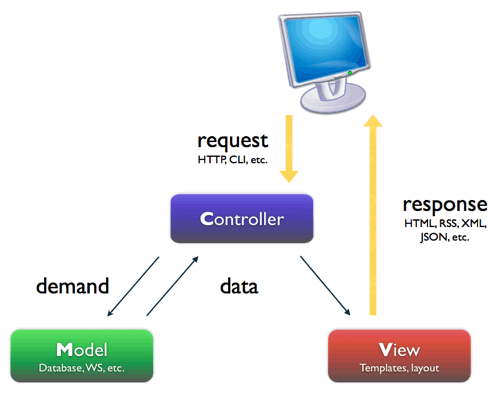
\includegraphics[width=8cm]{figs/mvc.png}
\end{center}

\begin{flushright}
{\footnotesize
Fuente: \url{http://djangoexamples.blogspot.com.es/2013/05/about-django-mvc.html}
}
\end{flushright}
\end{frame}

%%---------------------------------------------------------------
\begin{frame}
\frametitle{Model View Template (el de Django)}

\begin{center}
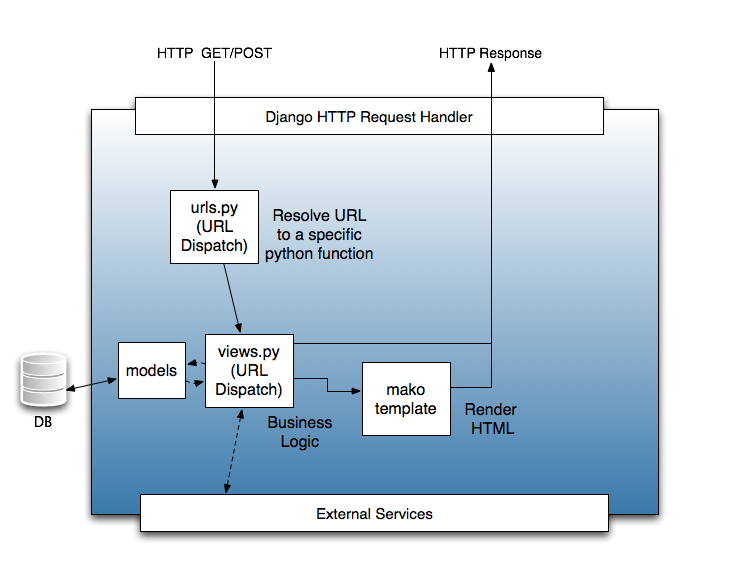
\includegraphics[width=8cm]{figs/mvt.png}
\end{center}

\begin{flushright}
{\footnotesize
Fuente: \url{http://archive.cloudera.com/cdh4/cdh/4/hue/sdk/sdk.html}
}
\end{flushright}
\end{frame}


%%---------------------------------------------------------------
\begin{frame}
\frametitle{Plantillas (templates)}

\begin{itemize}
\item Ficheros de texto que pueden generar cualquier formato basado en texto (HTML, XML, CSV, etc.)
\item Contienen:
  \begin{itemize}
  \item Texto (que queda igual)
  \item Variables (reemplazadas por su valor cuando se eval�an)
  \item Filtros (modifican variables cuando se eval�an)
  \item Etiquetas (controlan la l�gica de la evaluaci�n de la plantilla)
  \item Comentarios \{\# Comentario \#\}
  \end{itemize}
\item Pueden extender (heredar de) otras plantillas
\item Se colocan en los directorios de plantillas (TEMPLATE\_DIRS en settings.py) 
\end{itemize}
\end{frame}

%%---------------------------------------------------------------
\begin{frame}[fragile]
\frametitle{Plantillas: variables y filtros}

\begin{itemize}
\item Variables: 
\begin{verbatim}
    {{ variable }}
\end{verbatim}
\item Filtros:
\begin{verbatim}
    {{ variable|filtro|otrofiltro }}
\end{verbatim}
\item Filtro con argumentos:
\begin{verbatim}
    {{ variable|filtro:30 }}
\end{verbatim}
\item Ejemplos de filtros:
\begin{verbatim}
    {{ value|default:"nothing" }}
    {{ value|length }}
    {{ text|striptags }}
    {{ text|truncatewords:30 }}
    {{ text|escape|linebreaks }}
    {{ list|join:", " }}.
\end{verbatim}
\end{itemize}
\end{frame}

%%---------------------------------------------------------------
\begin{frame}[fragile]
\frametitle{Plantillas: etiquetas}

\begin{itemize}
\item for
\begin{verbatim}

    <li>{{ athlete.name }}</li>

\end{verbatim}
\item if
\begin{verbatim}

    Number of athletes: {{ athlete_list|length }}

    No athletes.

\end{verbatim}

\end{itemize}
\end{frame}

%%---------------------------------------------------------------
\begin{frame}[fragile]
\frametitle{Plantillas: etiquetas (2)}

\begin{itemize}
\item ifequal, ifnotequal
\begin{verbatim}

    ...


    ...

\end{verbatim}
\item block: Indica bloques a redefinir en plantillas que hereden
\item extends: Hereda de plantilla madre (s�lo hace falta redefinir
 \emph{blocks} que se quieren modificar)
\end{itemize}
\end{frame}


%%---------------------------------------------------------------

\begin{frame}[fragile]
\frametitle{Ficheros est�ticos con Django}

\begin{itemize}
\item Los ficheros est�ticos no se deber�an servir con Django...
\item (lo hace mucho mejor un servidor web como Apache o Cherokee)
\item ...pero se pueden servir
\item django.views.static.serve()

\begin{verbatim}
(r'^css/(?P<path>.*)$', 'django.views.static.serve',
        {'document_root': 'sfiles/css'}),
\end{verbatim}

\end{itemize}

\end{frame}


%%---------------------------------------------------------------
\begin{frame}[fragile]
\frametitle{Ejemplo de plantilla ``madre'' (base.html) (I)}

\begin{verbatim}
<!DOCTYPE html>
<html lang="en">
<head>
  <link rel="stylesheet" href="style.css" />
  <title>
    
      My amazing site
    
  </title>
</head>
\end{verbatim}

(sigue en la siguiente transparencia)

\end{frame}


%%---------------------------------------------------------------
\begin{frame}[fragile]
\frametitle{Ejemplo de plantilla ``madre'' (base.html) (II)}

\begin{verbatim}
<body>
  <div id="sidebar">
  
    <ul>
     <li><a href="/">Home</a></li>
     <li><a href="/blog/">Blog</a></li>
    </ul>
  
  </div>

  <div id="content">
     
  </div>
</body>
</html>
\end{verbatim}

\end{frame}


%%---------------------------------------------------------------
\begin{frame}[fragile]
\frametitle{Ejemplo de plantilla que hereda (plantilla.html)}

\begin{verbatim}


  {{ title }}



  <h1>{{ title }}</h1>
  
  <h2>
    <a href="{{ story.get_absolute_url }}">
      {{ story.headline|upper }}
    </a>
  </h2>
  <p>{{ story.tease|truncatewords:"100" }}</p>
  

\end{verbatim}

\end{frame}



%%---------------------------------------------------------------
\begin{frame}[fragile]
\frametitle{Plantillas: uso en vistas}

Directorios con plantillas: lista TEMPLATE\_DIRS en settings.py
 
\begin{verbatim}
from django.template.loader import get_template
from django.template import Context

def show_annotated_content(request, resource):
    ...
    template = get_template("annotated.html")
    return HttpResponse(template.render(
      Context({'user': user,
               'resource': resource,
               'page': page})))
\end{verbatim}
\end{frame}


%%---------------------------------------------------------------
\begin{frame}[fragile]
\frametitle{Plantillas: uso en urls.py}

\begin{verbatim}
from django.conf.urls.defaults import *
from django.views.generic.simple import direct_to_template

urlpatterns = patterns('',

    url(r'^about$', direct_to_template, {
        'template': 'about.html'
    }),
)
\end{verbatim}
\end{frame}

%%---------------------------------------------------------------
\begin{frame}[fragile]
\frametitle{Otras acciones de gesti�n del proyecto}

\begin{itemize}
\item Ejecuci�n en el contexto de Python con acceso al c�digo de la aplicaci�n
\begin{verbatim}
% python manage.py shell
\end{verbatim}
\item Validacion de modelos de datos
\begin{verbatim}
% python manage.py validate
\end{verbatim}
\item Exportaci�n de datos de la base de datos
\begin{verbatim}
% python manage.py dumpdata
\end{verbatim}
\item Importaci�n de datos en la base de datos
\begin{verbatim}
% python manage.py loaddata
\end{verbatim}
\end{itemize}

\end{frame}



%%---------------------------------------------------------------
\begin{frame}[fragile]
\frametitle{La shell de Django}

Acceso a la API de los objetos de nuestro proyecto

\begin{verbatim}
% python manage.py shell
>>> from myproject.myfirstapp.models import MyFirstAppData
>>> MyFirstAppData.objects.all()
[]
>>> p = MyFirstAppData(name="Jesus",
                       birthday="2009-05-05")
>>> p.save()
>>> p.id
1
>>> MyFirstAppData.objects.filter(name="Jesus")
...
>>> MyFirstAppData.objects.get(pk=1).name
u'Jesus'
\end{verbatim}

\end{frame}



%%---------------------------------------------------------------

\begin{frame}[fragile]
\frametitle{Modelos: relaci�n muchos a uno (ForeignKey)}

\begin{verbatim}
class Manufacturer(models.Model):
    # ...
class Car(models.Model):
    manufacturer = models.ForeignKey(Manufacturer)
    # ...
\end{verbatim}


\begin{verbatim}
# Creating
m = Manufacturer(name='Seat')
c = Car(name='Toledo')
m.save(); c.save()
# Relationship
c.manufacturer = m
# Obtaining
c.manufacturer
c.manufacturer.id
\end{verbatim}

\end{frame}

%%---------------------------------------------------------------

\begin{frame}[fragile]
\frametitle{Modelos: relaci�n muchos a muchos (ManyToManyField)}

\begin{verbatim}
class Topping(models.Model):
    # ...
class Pizza(models.Model):
    # ...
    toppings = models.ManyToManyField(Topping)
\end{verbatim}

\end{frame}

%%---------------------------------------------------------------

\begin{frame}[fragile]
\frametitle{Modelos: relaci�n muchos a muchos (ManyToManyField) (2)}

\begin{verbatim}
pb = Pizza(name='Barbecue')
pq = Pizza(name='4 Cheese')
b = Topping(name='Barbecue sauce')
m = Topping(name='Mozzarela')
pb.save(); pp.save(); b.save(); m.save()
pb.toppings.add(b, m)
pq.toppings.add(m)
pq.toppings.create(name='Rochefort')
m.pizza_set.all()
pb.toppings.all()
Pizza.objects.filter(toppings__name='Mozzarela')
\end{verbatim}

\end{frame}


%%---------------------------------------------------------------

\begin{frame}[fragile]
\frametitle{Generador de canales}

\begin{itemize}
\item Django viene con m�dulos para generar canales RSS y Atom
\item View de alto nivel que genera el canal (feed):

\begin{verbatim}
(r'^feeds/(?P<url>.*)/$', 'django.contrib.syndication.views.feed',
   {'feed_dict': feeds}),
\end{verbatim}

\item Hay que proporcionar un diccionario con la correspondencia canal a objeto Feed:

\begin{verbatim}
feeds = {
    'latest': LatestEntries,
    'categories': LatestEntriesByCategory,
}
\end{verbatim}
\end{itemize}

\end{frame}

%%---------------------------------------------------------------

\begin{frame}[fragile]
\frametitle{Generador de canales: objetos Feed}

\begin{itemize}
\item Representan los datos de un canal:

\begin{verbatim}
from django.contrib.syndication.feeds import Feed
from content.models import Pages

class LatestEntries(Feed):
    title = "My CMS contents"
    link = "/feed/"
    description = "Contents of my CMS."

    def items(self):
        return Pages.objects.order_by('-pub_date')[:5]
\end{verbatim}

\item Tambi�n hay que definir plantillas (templates) para $<$title$>$ y $<$description$>$ de cada item del canal RSS
\end{itemize}

\end{frame}

%%---------------------------------------------------------------

\begin{frame}[fragile]
\frametitle{Internacionalizaci�n}

\begin{itemize}
\item Cadenas de traducci�n en c�digo Python

\begin{verbatim}
from django.utils.translation import ugettext as _

def my_view(request):
    output = _("Welcome to my site.")
    return HttpResponse(output)

def my_view(request, m, d):
    output = _('Today is %(month)s, %(day)s.') % 
       {'month': m, 'day': d}
    return HttpResponse(output)
\end{verbatim}

\end{itemize}

\end{frame}

%%---------------------------------------------------------------

\begin{frame}[fragile]
\frametitle{Internacionalizaci�n (2)}

\begin{itemize}
\item Cadenas de traducci�n en plantillas

\begin{verbatim}
<title></title>


This string will have {{ value }} inside.

\end{verbatim}

\end{itemize}

\end{frame}

%%---------------------------------------------------------------

\begin{frame}[fragile]
\frametitle{Internacionalizaci�n (3)}

\begin{itemize}
\item Traducciones en los lenguajes requeridos

\begin{verbatim}
django-admin.py makemessages -l es
\end{verbatim}

\item Activar el soporte para locale en Django

\begin{verbatim}
MIDDLEWARE_CLASSES = (
 'django.contrib.sessions.middleware.SessionMiddleware',
 'django.middleware.locale.LocaleMiddleware',
 'django.middleware.common.CommonMiddleware',
)
\end{verbatim}

\end{itemize}

\end{frame}

%%---------------------------------------------------------------
\begin{frame}
\frametitle{Referencias}

\begin{itemize}
\item Documentaci�n de Django \\
  \url{http://docs.djangoproject.com/en/dev}
\item Libro de Django \\
  \url{http://www.djangobook.com}
\item Documentaci�n de Python \\
  \url{http://www.python.org/doc/}
\item Tutorial sobre Django (e introducci�n a Django) \\
\url{http://docs.djangoproject.com/en/dev/intro}
\end{itemize}

\end{frame}




\end{document}
